%********************************************%
%*       Generated from PreTeXt source      *%
%*       on 2021-04-05T10:30:07-05:00       *%
%*   A recent stable commit (2020-08-09):   *%
%* 98f21740783f166a773df4dc83cab5293ab63a4a *%
%*                                          *%
%*         https://pretextbook.org          *%
%*                                          *%
%********************************************%
%% We elect to always write snapshot output into <job>.dep file
\RequirePackage{snapshot}
\documentclass[oneside,10pt,]{book}
%% Custom Preamble Entries, early (use latex.preamble.early)
%% Default LaTeX packages
%%   1.  always employed (or nearly so) for some purpose, or
%%   2.  a stylewriter may assume their presence
\usepackage{geometry}
%% Some aspects of the preamble are conditional,
%% the LaTeX engine is one such determinant
\usepackage{ifthen}
%% etoolbox has a variety of modern conveniences
\usepackage{etoolbox}
\usepackage{ifxetex,ifluatex}
%% Raster graphics inclusion
\usepackage{graphicx}
%% Color support, xcolor package
%% Always loaded, for: add/delete text, author tools
%% Here, since tcolorbox loads tikz, and tikz loads xcolor
\PassOptionsToPackage{usenames,dvipsnames,svgnames,table}{xcolor}
\usepackage{xcolor}
%% begin: defined colors, via xcolor package, for styling
%% end: defined colors, via xcolor package, for styling
%% Colored boxes, and much more, though mostly styling
%% skins library provides "enhanced" skin, employing tikzpicture
%% boxes may be configured as "breakable" or "unbreakable"
%% "raster" controls grids of boxes, aka side-by-side
\usepackage{tcolorbox}
\tcbuselibrary{skins}
\tcbuselibrary{breakable}
\tcbuselibrary{raster}
%% We load some "stock" tcolorbox styles that we use a lot
%% Placement here is provisional, there will be some color work also
%% First, black on white, no border, transparent, but no assumption about titles
\tcbset{ bwminimalstyle/.style={size=minimal, boxrule=-0.3pt, frame empty,
colback=white, colbacktitle=white, coltitle=black, opacityfill=0.0} }
%% Second, bold title, run-in to text/paragraph/heading
%% Space afterwards will be controlled by environment,
%% independent of constructions of the tcb title
%% Places \blocktitlefont onto many block titles
\tcbset{ runintitlestyle/.style={fonttitle=\blocktitlefont\upshape\bfseries, attach title to upper} }
%% Spacing prior to each exercise, anywhere
\tcbset{ exercisespacingstyle/.style={before skip={1.5ex plus 0.5ex}} }
%% Spacing prior to each block
\tcbset{ blockspacingstyle/.style={before skip={2.0ex plus 0.5ex}} }
%% xparse allows the construction of more robust commands,
%% this is a necessity for isolating styling and behavior
%% The tcolorbox library of the same name loads the base library
\tcbuselibrary{xparse}
%% Hyperref should be here, but likes to be loaded late
%%
%% Inline math delimiters, \(, \), need to be robust
%% 2016-01-31:  latexrelease.sty  supersedes  fixltx2e.sty
%% If  latexrelease.sty  exists, bugfix is in kernel
%% If not, bugfix is in  fixltx2e.sty
%% See:  https://tug.org/TUGboat/tb36-3/tb114ltnews22.pdf
%% and read "Fewer fragile commands" in distribution's  latexchanges.pdf
\IfFileExists{latexrelease.sty}{}{\usepackage{fixltx2e}}
%% shorter subnumbers in some side-by-side require manipulations
\usepackage{xstring}
%% Footnote counters and part/chapter counters are manipulated
%% April 2018:  chngcntr  commands now integrated into the kernel,
%% but circa 2018/2019 the package would still try to redefine them,
%% so we need to do the work of loading conditionally for old kernels.
%% From version 1.1a,  chngcntr  should detect defintions made by LaTeX kernel.
\ifdefined\counterwithin
\else
    \usepackage{chngcntr}
\fi
%% Text height identically 9 inches, text width varies on point size
%% See Bringhurst 2.1.1 on measure for recommendations
%% 75 characters per line (count spaces, punctuation) is target
%% which is the upper limit of Bringhurst's recommendations
\geometry{letterpaper,total={340pt,9.0in}}
%% Custom Page Layout Adjustments (use latex.geometry)
%% This LaTeX file may be compiled with pdflatex, xelatex, or lualatex executables
%% LuaTeX is not explicitly supported, but we do accept additions from knowledgeable users
%% The conditional below provides  pdflatex  specific configuration last
%% begin: engine-specific capabilities
\ifthenelse{\boolean{xetex} \or \boolean{luatex}}{%
%% begin: xelatex and lualatex-specific default configuration
\ifxetex\usepackage{xltxtra}\fi
%% realscripts is the only part of xltxtra relevant to lualatex 
\ifluatex\usepackage{realscripts}\fi
%% end:   xelatex and lualatex-specific default configuration
}{
%% begin: pdflatex-specific default configuration
%% We assume a PreTeXt XML source file may have Unicode characters
%% and so we ask LaTeX to parse a UTF-8 encoded file
%% This may work well for accented characters in Western language,
%% but not with Greek, Asian languages, etc.
%% When this is not good enough, switch to the  xelatex  engine
%% where Unicode is better supported (encouraged, even)
\usepackage[utf8]{inputenc}
%% end: pdflatex-specific default configuration
}
%% end:   engine-specific capabilities
%%
%% Fonts.  Conditional on LaTex engine employed.
%% Default Text Font: The Latin Modern fonts are
%% "enhanced versions of the [original TeX] Computer Modern fonts."
%% We use them as the default text font for PreTeXt output.
%% Automatic Font Control
%% Portions of a document, are, or may, be affected by defined commands
%% These are perhaps more flexible when using  xelatex  rather than  pdflatex
%% The following definitions are meant to be re-defined in a style, using \renewcommand
%% They are scoped when employed (in a TeX group), and so should not be defined with an argument
\newcommand{\divisionfont}{\relax}
\newcommand{\blocktitlefont}{\relax}
\newcommand{\contentsfont}{\relax}
\newcommand{\pagefont}{\relax}
\newcommand{\tabularfont}{\relax}
\newcommand{\xreffont}{\relax}
\newcommand{\titlepagefont}{\relax}
%%
\ifthenelse{\boolean{xetex} \or \boolean{luatex}}{%
%% begin: font setup and configuration for use with xelatex
%% Generally, xelatex is necessary for non-Western fonts
%% fontspec package provides extensive control of system fonts,
%% meaning *.otf (OpenType), and apparently *.ttf (TrueType)
%% that live *outside* your TeX/MF tree, and are controlled by your *system*
%% (it is possible that a TeX distribution will place fonts in a system location)
%%
%% The fontspec package is the best vehicle for using different fonts in  xelatex
%% So we load it always, no matter what a publisher or style might want
%%
\usepackage{fontspec}
%%
%% begin: xelatex main font ("font-xelatex-main" template)
%% Latin Modern Roman is the default font for xelatex and so is loaded with a TU encoding
%% *in the format* so we can't touch it, only perhaps adjust it later
%% in one of two ways (then known by NFSS names such as "lmr")
%% (1) via NFSS with font family names such as "lmr" and "lmss"
%% (2) via fontspec with commands like \setmainfont{Latin Modern Roman}
%% The latter requires the font to be known at the system-level by its font name,
%% but will give access to OTF font features through optional arguments
%% https://tex.stackexchange.com/questions/470008/
%% where-and-how-does-fontspec-sty-specify-the-default-font-latin-modern-roman
%% http://tex.stackexchange.com/questions/115321
%% /how-to-optimize-latin-modern-font-with-xelatex
%%
%% end:   xelatex main font ("font-xelatex-main" template)
%% begin: xelatex mono font ("font-xelatex-mono" template)
%% (conditional on non-trivial uses being present in source)
%% end:   xelatex mono font ("font-xelatex-mono" template)
%% begin: xelatex font adjustments ("font-xelatex-style" template)
%% end:   xelatex font adjustments ("font-xelatex-style" template)
%%
%% Extensive support for other languages
\usepackage{polyglossia}
%% Set main/default language based on pretext/@xml:lang value
%% document language code is "en-US", US English
%% usmax variant has extra hypenation
\setmainlanguage[variant=usmax]{english}
%% Enable secondary languages based on discovery of @xml:lang values
%% Enable fonts/scripts based on discovery of @xml:lang values
%% Western languages should be ably covered by Latin Modern Roman
%% end:   font setup and configuration for use with xelatex
}{%
%% begin: font setup and configuration for use with pdflatex
%% begin: pdflatex main font ("font-pdflatex-main" template)
\usepackage{lmodern}
\usepackage[T1]{fontenc}
%% end:   pdflatex main font ("font-pdflatex-main" template)
%% begin: pdflatex mono font ("font-pdflatex-mono" template)
%% (conditional on non-trivial uses being present in source)
%% end:   pdflatex mono font ("font-pdflatex-mono" template)
%% begin: pdflatex font adjustments ("font-pdflatex-style" template)
%% end:   pdflatex font adjustments ("font-pdflatex-style" template)
%% end:   font setup and configuration for use with pdflatex
}
%% Micromanage spacing, etc.  The named "microtype-options"
%% template may be employed to fine-tune package behavior
\usepackage{microtype}
%% Symbols, align environment, commutative diagrams, bracket-matrix
\usepackage{amsmath}
\usepackage{amscd}
\usepackage{amssymb}
%% allow page breaks within display mathematics anywhere
%% level 4 is maximally permissive
%% this is exactly the opposite of AMSmath package philosophy
%% there are per-display, and per-equation options to control this
%% split, aligned, gathered, and alignedat are not affected
\allowdisplaybreaks[4]
%% allow more columns to a matrix
%% can make this even bigger by overriding with  latex.preamble.late  processing option
\setcounter{MaxMatrixCols}{30}
%%
%%
%% Division Titles, and Page Headers/Footers
%% titlesec package, loading "titleps" package cooperatively
%% See code comments about the necessity and purpose of "explicit" option.
%% The "newparttoc" option causes a consistent entry for parts in the ToC 
%% file, but it is only effective if there is a \titleformat for \part.
%% "pagestyles" loads the  titleps  package cooperatively.
\usepackage[explicit, newparttoc, pagestyles]{titlesec}
%% The companion titletoc package for the ToC.
\usepackage{titletoc}
%% Fixes a bug with transition from chapters to appendices in a "book"
%% See generating XSL code for more details about necessity
\newtitlemark{\chaptertitlename}
%% begin: customizations of page styles via the modal "titleps-style" template
%% Designed to use commands from the LaTeX "titleps" package
%% Plain pages should have the same font for page numbers
\renewpagestyle{plain}{%
\setfoot{}{\pagefont\thepage}{}%
}%
%% Single pages as in default LaTeX
\renewpagestyle{headings}{%
\sethead{\pagefont\slshape\MakeUppercase{\ifthechapter{\chaptertitlename\space\thechapter.\space}{}\chaptertitle}}{}{\pagefont\thepage}%
}%
\pagestyle{headings}
%% end: customizations of page styles via the modal "titleps-style" template
%%
%% Create globally-available macros to be provided for style writers
%% These are redefined for each occurence of each division
\newcommand{\divisionnameptx}{\relax}%
\newcommand{\titleptx}{\relax}%
\newcommand{\subtitleptx}{\relax}%
\newcommand{\shortitleptx}{\relax}%
\newcommand{\authorsptx}{\relax}%
\newcommand{\epigraphptx}{\relax}%
%% Create environments for possible occurences of each division
%% Environment for a PTX "acknowledgement" at the level of a LaTeX "chapter"
\NewDocumentEnvironment{acknowledgement}{mmmmmm}
{%
\renewcommand{\divisionnameptx}{Acknowledgements}%
\renewcommand{\titleptx}{#1}%
\renewcommand{\subtitleptx}{#2}%
\renewcommand{\shortitleptx}{#3}%
\renewcommand{\authorsptx}{#4}%
\renewcommand{\epigraphptx}{#5}%
\chapter*{#1}%
\addcontentsline{toc}{chapter}{#3}
\label{#6}%
}{}%
%% Environment for a PTX "preface" at the level of a LaTeX "chapter"
\NewDocumentEnvironment{preface}{mmmmmm}
{%
\renewcommand{\divisionnameptx}{Preface}%
\renewcommand{\titleptx}{#1}%
\renewcommand{\subtitleptx}{#2}%
\renewcommand{\shortitleptx}{#3}%
\renewcommand{\authorsptx}{#4}%
\renewcommand{\epigraphptx}{#5}%
\chapter*{#1}%
\addcontentsline{toc}{chapter}{#3}
\label{#6}%
}{}%
%% Environment for a PTX "chapter" at the level of a LaTeX "chapter"
\NewDocumentEnvironment{chapterptx}{mmmmmm}
{%
\renewcommand{\divisionnameptx}{Chapter}%
\renewcommand{\titleptx}{#1}%
\renewcommand{\subtitleptx}{#2}%
\renewcommand{\shortitleptx}{#3}%
\renewcommand{\authorsptx}{#4}%
\renewcommand{\epigraphptx}{#5}%
\chapter[{#3}]{#1}%
\label{#6}%
}{}%
%% Environment for a PTX "section" at the level of a LaTeX "section"
\NewDocumentEnvironment{sectionptx}{mmmmmm}
{%
\renewcommand{\divisionnameptx}{Section}%
\renewcommand{\titleptx}{#1}%
\renewcommand{\subtitleptx}{#2}%
\renewcommand{\shortitleptx}{#3}%
\renewcommand{\authorsptx}{#4}%
\renewcommand{\epigraphptx}{#5}%
\section[{#3}]{#1}%
\label{#6}%
}{}%
%% Environment for a PTX "subsection" at the level of a LaTeX "subsection"
\NewDocumentEnvironment{subsectionptx}{mmmmmm}
{%
\renewcommand{\divisionnameptx}{Subsection}%
\renewcommand{\titleptx}{#1}%
\renewcommand{\subtitleptx}{#2}%
\renewcommand{\shortitleptx}{#3}%
\renewcommand{\authorsptx}{#4}%
\renewcommand{\epigraphptx}{#5}%
\subsection[{#3}]{#1}%
\label{#6}%
}{}%
%% Environment for a PTX "subsubsection" at the level of a LaTeX "subsubsection"
\NewDocumentEnvironment{subsubsectionptx}{mmmmmm}
{%
\renewcommand{\divisionnameptx}{Subsubsection}%
\renewcommand{\titleptx}{#1}%
\renewcommand{\subtitleptx}{#2}%
\renewcommand{\shortitleptx}{#3}%
\renewcommand{\authorsptx}{#4}%
\renewcommand{\epigraphptx}{#5}%
\subsubsection[{#3}]{#1}%
\label{#6}%
}{}%
%% Environment for a PTX "exercises" at the level of a LaTeX "subsection"
\NewDocumentEnvironment{exercises-subsection}{mmmmmm}
{%
\renewcommand{\divisionnameptx}{Exercises}%
\renewcommand{\titleptx}{#1}%
\renewcommand{\subtitleptx}{#2}%
\renewcommand{\shortitleptx}{#3}%
\renewcommand{\authorsptx}{#4}%
\renewcommand{\epigraphptx}{#5}%
\subsection[{#3}]{#1}%
\label{#6}%
}{}%
%% Environment for a PTX "exercises" at the level of a LaTeX "subsection"
\NewDocumentEnvironment{exercises-subsection-numberless}{mmmmmm}
{%
\renewcommand{\divisionnameptx}{Exercises}%
\renewcommand{\titleptx}{#1}%
\renewcommand{\subtitleptx}{#2}%
\renewcommand{\shortitleptx}{#3}%
\renewcommand{\authorsptx}{#4}%
\renewcommand{\epigraphptx}{#5}%
\subsection*{#1}%
\addcontentsline{toc}{subsection}{#3}
\label{#6}%
}{}%
%% Environment for a PTX "index" at the level of a LaTeX "chapter"
\NewDocumentEnvironment{indexptx}{mmmmmm}
{%
\renewcommand{\divisionnameptx}{Index}%
\renewcommand{\titleptx}{#1}%
\renewcommand{\subtitleptx}{#2}%
\renewcommand{\shortitleptx}{#3}%
\renewcommand{\authorsptx}{#4}%
\renewcommand{\epigraphptx}{#5}%
\chapter*{#1}%
\addcontentsline{toc}{chapter}{#3}
\label{#6}%
}{}%
%% Environment for a PTX "appendix" at the level of a LaTeX "chapter"
\NewDocumentEnvironment{appendixptx}{mmmmmm}
{%
\renewcommand{\divisionnameptx}{Appendix}%
\renewcommand{\titleptx}{#1}%
\renewcommand{\subtitleptx}{#2}%
\renewcommand{\shortitleptx}{#3}%
\renewcommand{\authorsptx}{#4}%
\renewcommand{\epigraphptx}{#5}%
\chapter[{#3}]{#1}%
\label{#6}%
}{}%
%%
%% Styles for six traditional LaTeX divisions
\titleformat{\part}[display]
{\divisionfont\Huge\bfseries\centering}{\divisionnameptx\space\thepart}{30pt}{\Huge#1}
[{\Large\centering\authorsptx}]
\titleformat{\chapter}[display]
{\divisionfont\huge\bfseries}{\divisionnameptx\space\thechapter}{20pt}{\Huge#1}
[{\Large\authorsptx}]
\titleformat{name=\chapter,numberless}[display]
{\divisionfont\huge\bfseries}{}{0pt}{#1}
[{\Large\authorsptx}]
\titlespacing*{\chapter}{0pt}{50pt}{40pt}
\titleformat{\section}[hang]
{\divisionfont\Large\bfseries}{\thesection}{1ex}{#1}
[{\large\authorsptx}]
\titleformat{name=\section,numberless}[block]
{\divisionfont\Large\bfseries}{}{0pt}{#1}
[{\large\authorsptx}]
\titlespacing*{\section}{0pt}{3.5ex plus 1ex minus .2ex}{2.3ex plus .2ex}
\titleformat{\subsection}[hang]
{\divisionfont\large\bfseries}{\thesubsection}{1ex}{#1}
[{\normalsize\authorsptx}]
\titleformat{name=\subsection,numberless}[block]
{\divisionfont\large\bfseries}{}{0pt}{#1}
[{\normalsize\authorsptx}]
\titlespacing*{\subsection}{0pt}{3.25ex plus 1ex minus .2ex}{1.5ex plus .2ex}
\titleformat{\subsubsection}[hang]
{\divisionfont\normalsize\bfseries}{\thesubsubsection}{1em}{#1}
[{\small\authorsptx}]
\titleformat{name=\subsubsection,numberless}[block]
{\divisionfont\normalsize\bfseries}{}{0pt}{#1}
[{\normalsize\authorsptx}]
\titlespacing*{\subsubsection}{0pt}{3.25ex plus 1ex minus .2ex}{1.5ex plus .2ex}
\titleformat{\paragraph}[hang]
{\divisionfont\normalsize\bfseries}{\theparagraph}{1em}{#1}
[{\small\authorsptx}]
\titleformat{name=\paragraph,numberless}[block]
{\divisionfont\normalsize\bfseries}{}{0pt}{#1}
[{\normalsize\authorsptx}]
\titlespacing*{\paragraph}{0pt}{3.25ex plus 1ex minus .2ex}{1.5em}
%%
%% Styles for five traditional LaTeX divisions
\titlecontents{part}%
[0pt]{\contentsmargin{0em}\addvspace{1pc}\contentsfont\bfseries}%
{\Large\thecontentslabel\enspace}{\Large}%
{}%
[\addvspace{.5pc}]%
\titlecontents{chapter}%
[0pt]{\contentsmargin{0em}\addvspace{1pc}\contentsfont\bfseries}%
{\large\thecontentslabel\enspace}{\large}%
{\hfill\bfseries\thecontentspage}%
[\addvspace{.5pc}]%
\dottedcontents{section}[3.8em]{\contentsfont}{2.3em}{1pc}%
\dottedcontents{subsection}[6.1em]{\contentsfont}{3.2em}{1pc}%
\dottedcontents{subsubsection}[9.3em]{\contentsfont}{4.3em}{1pc}%
%%
%% Begin: Semantic Macros
%% To preserve meaning in a LaTeX file
%%
%% \mono macro for content of "c", "cd", "tag", etc elements
%% Also used automatically in other constructions
%% Simply an alias for \texttt
%% Always defined, even if there is no need, or if a specific tt font is not loaded
\newcommand{\mono}[1]{\texttt{#1}}
%%
%% Following semantic macros are only defined here if their
%% use is required only in this specific document
%%
%% Used for inline definitions of terms
\newcommand{\terminology}[1]{\textbf{#1}}
%% End: Semantic Macros
%% Divisional exercises (and worksheet) as LaTeX environments
%% Third argument is option for extra workspace in worksheets
%% Hanging indent occupies a 5ex width slot prior to left margin
%% Experimentally this seems just barely sufficient for a bold "888."
%% Division exercises, not in exercise group
\tcbset{ divisionexercisestyle/.style={bwminimalstyle, runintitlestyle, exercisespacingstyle, left=5ex, breakable, parbox=false } }
\newtcolorbox{divisionexercise}[4]{divisionexercisestyle, before title={\hspace{-5ex}\makebox[5ex][l]{#1.}}, title={\notblank{#2}{#2\space}{}}, phantom={\hypertarget{#4}{}}, after={\notblank{#3}{\newline\rule{\workspacestrutwidth}{#3\textheight}\newline}{}}}
%% Localize LaTeX supplied names (possibly none)
\renewcommand*{\appendixname}{Appendix}
\renewcommand*{\chaptername}{Chapter}
%% Equation Numbering
%% Controlled by  numbering.equations.level  processing parameter
%% No adjustment here implies document-wide numbering
\numberwithin{equation}{section}
%% "tcolorbox" environment for a single image, occupying entire \linewidth
%% arguments are left-margin, width, right-margin, as multiples of
%% \linewidth, and are guaranteed to be positive and sum to 1.0
\tcbset{ imagestyle/.style={bwminimalstyle} }
\NewTColorBox{image}{mmm}{imagestyle,left skip=#1\linewidth,width=#2\linewidth}
%% For improved tables
\usepackage{array}
%% Some extra height on each row is desirable, especially with horizontal rules
%% Increment determined experimentally
\setlength{\extrarowheight}{0.2ex}
%% Define variable thickness horizontal rules, full and partial
%% Thicknesses are 0.03, 0.05, 0.08 in the  booktabs  package
\newcommand{\hrulethin}  {\noalign{\hrule height 0.04em}}
\newcommand{\hrulemedium}{\noalign{\hrule height 0.07em}}
\newcommand{\hrulethick} {\noalign{\hrule height 0.11em}}
%% We preserve a copy of the \setlength package before other
%% packages (extpfeil) get a chance to load packages that redefine it
\let\oldsetlength\setlength
\newlength{\Oldarrayrulewidth}
\newcommand{\crulethin}[1]%
{\noalign{\global\oldsetlength{\Oldarrayrulewidth}{\arrayrulewidth}}%
\noalign{\global\oldsetlength{\arrayrulewidth}{0.04em}}\cline{#1}%
\noalign{\global\oldsetlength{\arrayrulewidth}{\Oldarrayrulewidth}}}%
\newcommand{\crulemedium}[1]%
{\noalign{\global\oldsetlength{\Oldarrayrulewidth}{\arrayrulewidth}}%
\noalign{\global\oldsetlength{\arrayrulewidth}{0.07em}}\cline{#1}%
\noalign{\global\oldsetlength{\arrayrulewidth}{\Oldarrayrulewidth}}}
\newcommand{\crulethick}[1]%
{\noalign{\global\oldsetlength{\Oldarrayrulewidth}{\arrayrulewidth}}%
\noalign{\global\oldsetlength{\arrayrulewidth}{0.11em}}\cline{#1}%
\noalign{\global\oldsetlength{\arrayrulewidth}{\Oldarrayrulewidth}}}
%% Single letter column specifiers defined via array package
\newcolumntype{A}{!{\vrule width 0.04em}}
\newcolumntype{B}{!{\vrule width 0.07em}}
\newcolumntype{C}{!{\vrule width 0.11em}}
%% tcolorbox to place tabular outside of a sidebyside
\tcbset{ tabularboxstyle/.style={bwminimalstyle,} }
\newtcolorbox{tabularbox}[3]{tabularboxstyle, left skip=#1\linewidth, width=#2\linewidth,}
%% Footnote Numbering
%% Specified by numbering.footnotes.level
%% Undo counter reset by chapter for a book
\counterwithout{footnote}{chapter}
\counterwithin*{footnote}{section}
%% QR Code Support
%% Videos and other interactives
\usepackage{qrcode}
\newlength{\qrsize}
\newlength{\previewwidth}
%% tcolorbox styles for interactive previews
%% changing size= and/or colback can aid in debugging
\tcbset{ previewstyle/.style={bwminimalstyle, halign=center} }
\tcbset{ qrstyle/.style={bwminimalstyle, hbox} }
\tcbset{ captionstyle/.style={bwminimalstyle, left=1em, width=\linewidth} }
%% Generic red play button (from SVG)
%% tikz package should be loaded by now
\definecolor{playred}{RGB}{230,33,23}
\newcommand{\genericpreview}{
        \begin{tikzpicture}[y=0.80pt, x=0.80pt, yscale=-1.000000, xscale=1.000000, inner sep=0pt, outer sep=0pt]
        \path[fill=playred] (94.9800,28.8400) .. controls (94.9800,28.8400) and
        (94.0400,22.2400) .. (91.1700,19.3400) .. controls (87.5300,15.5300) and
        (83.4500,15.5100) .. (81.5800,15.2900) .. controls (68.1800,14.3200) and
        (48.0600,14.4400) .. (48.0600,14.4400) .. controls (48.0600,14.4400) and
        (27.9400,14.3200) .. (14.5400,15.2900) .. controls (12.6700,15.5100) and
        (8.5900,15.5300) .. (4.9500,19.3400) .. controls (2.0800,22.2400) and
        (1.1400,28.8400) .. (1.1400,28.8400) .. controls (1.1400,28.8400) and
        (0.1800,36.5800) .. (0.0000,44.3300) -- (0.0000,51.5900) .. controls
        (0.1800,59.3400) and (1.1400,67.0800) .. (1.1400,67.0800) .. controls
        (1.1400,67.0800) and (2.0700,73.6800) .. (4.9500,76.5800) .. controls
        (8.5900,80.3900) and (13.3800,80.2700) .. (15.5100,80.6700) .. controls
        (23.0400,81.3900) and (47.2100,81.5600) .. (48.0500,81.5700) .. controls
        (48.0600,81.5700) and (68.1900,81.6000) .. (81.5900,80.6300) .. controls
        (83.4600,80.4100) and (87.5400,80.3900) .. (91.1800,76.5800) .. controls
        (94.0500,73.6800) and (94.9900,67.0800) .. (94.9900,67.0800) .. controls
        (94.9900,67.0800) and (95.9500,59.3300) .. (96.0100,51.5900) --
        (96.0100,44.3300) .. controls (95.9400,36.5800) and (94.9800,28.8400) ..
        (94.9800,28.8400) -- cycle(38.2800,61.4100) -- (38.2800,34.4100) --
        (64.0200,47.9100) -- (38.2800,61.4100) -- cycle;
        \end{tikzpicture}
        }
%% Multiple column, column-major lists
\usepackage{multicol}
%% More flexible list management, esp. for references
%% But also for specifying labels (i.e. custom order) on nested lists
\usepackage{enumitem}
%% Support for index creation
%% imakeidx package does not require extra pass (as with makeidx)
%% Title of the "Index" section set via a keyword
%% Language support for the "see" and "see also" phrases
\usepackage{imakeidx}
\makeindex[title=Index, intoc=true]
\renewcommand{\seename}{See}
\renewcommand{\alsoname}{See also}
%% Package for tables spanning several pages
\usepackage{longtable}
%% hyperref driver does not need to be specified, it will be detected
%% Footnote marks in tcolorbox have broken linking under
%% hyperref, so it is necessary to turn off all linking
%% It *must* be given as a package option, not with \hypersetup
\usepackage[hyperfootnotes=false]{hyperref}
%% configure hyperref's  \url  to match listings' inline verbatim
\renewcommand\UrlFont{\small\ttfamily}
%% Hyperlinking active in electronic PDFs, all links solid and blue
\hypersetup{colorlinks=true,linkcolor=blue,citecolor=blue,filecolor=blue,urlcolor=blue}
\hypersetup{pdftitle={Discrete Structures Learning Guides}}
%% If you manually remove hyperref, leave in this next command
\providecommand\phantomsection{}
%% Division Numbering: Chapters, Sections, Subsections, etc
%% Division numbers may be turned off at some level ("depth")
%% A section *always* has depth 1, contrary to us counting from the document root
%% The latex default is 3.  If a larger number is present here, then
%% removing this command may make some cross-references ambiguous
%% The precursor variable $numbering-maxlevel is checked for consistency in the common XSL file
\setcounter{secnumdepth}{3}
%%
%% AMS "proof" environment is no longer used, but we leave previously
%% implemented \qedhere in place, should the LaTeX be recycled
\newcommand{\qedhere}{\relax}
%%
%% A faux tcolorbox whose only purpose is to provide common numbering
%% facilities for most blocks (possibly not projects, 2D displays)
%% Controlled by  numbering.theorems.level  processing parameter
\newtcolorbox[auto counter, number within=section]{block}{}
%%
%% This document is set to number PROJECT-LIKE on a separate numbering scheme
%% So, a faux tcolorbox whose only purpose is to provide this numbering
%% Controlled by  numbering.projects.level  processing parameter
\newtcolorbox[auto counter, number within=section]{project-distinct}{}
%% A faux tcolorbox whose only purpose is to provide common numbering
%% facilities for 2D displays which are subnumbered as part of a "sidebyside"
\makeatletter
\newtcolorbox[auto counter, number within=tcb@cnt@block, number freestyle={\noexpand\thetcb@cnt@block(\noexpand\alph{\tcbcounter})}]{subdisplay}{}
\makeatother
%%
%% tcolorbox, with styles, for THEOREM-LIKE
%%
%% theorem: fairly simple numbered block/structure
\tcbset{ theoremstyle/.style={bwminimalstyle, runintitlestyle, blockspacingstyle, after title={\space}, } }
\newtcolorbox[use counter from=block]{theorem}[3]{title={{Theorem~\thetcbcounter\notblank{#1#2}{\space}{}\notblank{#1}{\space#1}{}\notblank{#2}{\space(#2)}{}}}, phantomlabel={#3}, breakable, parbox=false, after={\par}, fontupper=\itshape, theoremstyle, }
%% proposition: fairly simple numbered block/structure
\tcbset{ propositionstyle/.style={bwminimalstyle, runintitlestyle, blockspacingstyle, after title={\space}, } }
\newtcolorbox[use counter from=block]{proposition}[3]{title={{Proposition~\thetcbcounter\notblank{#1#2}{\space}{}\notblank{#1}{\space#1}{}\notblank{#2}{\space(#2)}{}}}, phantomlabel={#3}, breakable, parbox=false, after={\par}, fontupper=\itshape, propositionstyle, }
%% lemma: fairly simple numbered block/structure
\tcbset{ lemmastyle/.style={bwminimalstyle, runintitlestyle, blockspacingstyle, after title={\space}, } }
\newtcolorbox[use counter from=block]{lemma}[3]{title={{Lemma~\thetcbcounter\notblank{#1#2}{\space}{}\notblank{#1}{\space#1}{}\notblank{#2}{\space(#2)}{}}}, phantomlabel={#3}, breakable, parbox=false, after={\par}, fontupper=\itshape, lemmastyle, }
%% corollary: fairly simple numbered block/structure
\tcbset{ corollarystyle/.style={bwminimalstyle, runintitlestyle, blockspacingstyle, after title={\space}, } }
\newtcolorbox[use counter from=block]{corollary}[3]{title={{Corollary~\thetcbcounter\notblank{#1#2}{\space}{}\notblank{#1}{\space#1}{}\notblank{#2}{\space(#2)}{}}}, phantomlabel={#3}, breakable, parbox=false, after={\par}, fontupper=\itshape, corollarystyle, }
%%
%% tcolorbox, with styles, for AXIOM-LIKE
%%
%% principle: fairly simple numbered block/structure
\tcbset{ principlestyle/.style={bwminimalstyle, runintitlestyle, blockspacingstyle, after title={\space}, } }
\newtcolorbox[use counter from=block]{principle}[3]{title={{Discussion~\thetcbcounter\notblank{#1#2}{\space}{}\notblank{#1}{\space#1}{}\notblank{#2}{\space(#2)}{}}}, phantomlabel={#3}, breakable, parbox=false, after={\par}, fontupper=\itshape, principlestyle, }
%%
%% tcolorbox, with styles, for DEFINITION-LIKE
%%
%% definition: fairly simple numbered block/structure
\tcbset{ definitionstyle/.style={bwminimalstyle, runintitlestyle, blockspacingstyle, after title={\space}, after upper={\space\space\hspace*{\stretch{1}}\(\lozenge\)}, } }
\newtcolorbox[use counter from=block]{definition}[2]{title={{Definition~\thetcbcounter\notblank{#1}{\space\space#1}{}}}, phantomlabel={#2}, breakable, parbox=false, after={\par}, definitionstyle, }
%%
%% tcolorbox, with styles, for REMARK-LIKE
%%
%% insight: fairly simple numbered block/structure
\tcbset{ insightstyle/.style={bwminimalstyle, runintitlestyle, blockspacingstyle, after title={\space}, } }
\newtcolorbox[use counter from=block]{insight}[2]{title={{Screencast~\thetcbcounter\notblank{#1}{\space\space#1}{}}}, phantomlabel={#2}, breakable, parbox=false, after={\par}, insightstyle, }
%% remark: fairly simple numbered block/structure
\tcbset{ remarkstyle/.style={bwminimalstyle, runintitlestyle, blockspacingstyle, after title={\space}, } }
\newtcolorbox[use counter from=block]{remark}[2]{title={{Remark~\thetcbcounter\notblank{#1}{\space\space#1}{}}}, phantomlabel={#2}, breakable, parbox=false, after={\par}, remarkstyle, }
%%
%% tcolorbox, with styles, for EXAMPLE-LIKE
%%
%% question: fairly simple numbered block/structure
\tcbset{ questionstyle/.style={bwminimalstyle, runintitlestyle, blockspacingstyle, after title={\space}, after upper={\space\space\hspace*{\stretch{1}}\(\square\)}, } }
\newtcolorbox[use counter from=block]{question}[2]{title={{Question~\thetcbcounter\notblank{#1}{\space\space#1}{}}}, phantomlabel={#2}, breakable, parbox=false, after={\par}, questionstyle, }
%% example: fairly simple numbered block/structure
\tcbset{ examplestyle/.style={bwminimalstyle, runintitlestyle, blockspacingstyle, after title={\space}, after upper={\space\space\hspace*{\stretch{1}}\(\square\)}, } }
\newtcolorbox[use counter from=block]{example}[2]{title={{Example~\thetcbcounter\notblank{#1}{\space\space#1}{}}}, phantomlabel={#2}, breakable, parbox=false, after={\par}, examplestyle, }
%%
%% tcolorbox, with styles, for PROJECT-LIKE
%%
%% exploration: fairly simple numbered block/structure
\tcbset{ explorationstyle/.style={bwminimalstyle, runintitlestyle, blockspacingstyle, after title={\space}, } }
\newtcolorbox[use counter from=project-distinct]{exploration}[2]{title={{Exploration~\thetcbcounter\notblank{#1}{\space\space#1}{}}}, phantomlabel={#2}, breakable, parbox=false, after={\par}, explorationstyle, }
%% activity: fairly simple numbered block/structure
\tcbset{ activitystyle/.style={bwminimalstyle, runintitlestyle, blockspacingstyle, after title={\space}, } }
\newtcolorbox[use counter from=project-distinct]{activity}[2]{title={{Activity~\thetcbcounter\notblank{#1}{\space\space#1}{}}}, phantomlabel={#2}, breakable, parbox=false, after={\par}, activitystyle, }
%% investigation: fairly simple numbered block/structure
\tcbset{ investigationstyle/.style={bwminimalstyle, runintitlestyle, blockspacingstyle, after title={\space}, } }
\newtcolorbox[use counter from=project-distinct]{investigation}[2]{title={{Investigation~\thetcbcounter\notblank{#1}{\space\space#1}{}}}, phantomlabel={#2}, breakable, parbox=false, after={\par}, investigationstyle, }
%%
%% tcolorbox, with styles, for ASIDE-LIKE
%%
%% aside: fairly simple un-numbered block/structure
\tcbset{ asidestyle/.style={bwminimalstyle, runintitlestyle, blockspacingstyle, after title={\space}, } }
\newtcolorbox{aside}[2]{title={\notblank{#1}{#1}{}}, phantomlabel={#2}, breakable, parbox=false, asidestyle}
%%
%% xparse environments for introductions and conclusions of divisions
%%
%% introduction: in a structured division
\NewDocumentEnvironment{introduction}{m}
{\notblank{#1}{\noindent\textbf{#1}\space}{}}{\par\medskip}
%%
%% tcolorbox, with styles, for miscellaneous environments
%%
%% assemblage: fairly simple un-numbered block/structure
\tcbset{ assemblagestyle/.style={size=normal, colback=white, colbacktitle=white, coltitle=black, colframe=black, rounded corners, titlerule=0.0pt, center title, fonttitle=\blocktitlefont\bfseries, blockspacingstyle, } }
\newtcolorbox{assemblage}[2]{title={\notblank{#1}{#1}{}}, phantomlabel={#2}, breakable, parbox=false, assemblagestyle}
\NewDocumentEnvironment{solutionproof}{}
{\par\smallskip\noindent\textit{Proof}.\space\space}{\space\space\hspace*{\stretch{1}}\(\blacksquare\)\par\smallskip}
%% proof: title is a replacement
\tcbset{ proofstyle/.style={bwminimalstyle, fonttitle=\blocktitlefont\itshape, attach title to upper, after title={\space}, after upper={\space\space\hspace*{\stretch{1}}\(\blacksquare\)},
} }
\newtcolorbox{proof}[2]{title={\notblank{#1}{#1}{Proof.}}, phantom={\hypertarget{#2}{}}, breakable, parbox=false, after={\par}, proofstyle }
%% paragraphs: the terminal, pseudo-division
%% We use the lowest LaTeX traditional division
\titleformat{\subparagraph}[runin]{\normalfont\normalsize\bfseries}{\thesubparagraph}{1em}{#1}
\titlespacing*{\subparagraph}{0pt}{3.25ex plus 1ex minus .2ex}{1em}
\NewDocumentEnvironment{paragraphs}{mm}
{\subparagraph*{#1}\hypertarget{#2}{}}{}
%% Graphics Preamble Entries
\usepackage{tikz}
\usepackage{url}
\usepackage{tkz-graph}
\usepackage{tkz-euclide}
\usetikzlibrary{patterns}
\usetikzlibrary{positioning}
\usetikzlibrary{matrix,arrows}
\usetikzlibrary{calc}
\usetikzlibrary{shapes}
\usetikzlibrary{through,intersections,decorations,shadows,fadings}
\usepackage{pgfplots}
%% If tikz has been loaded, replace ampersand with \amp macro
\ifdefined\tikzset
    \tikzset{ampersand replacement = \amp}
\fi
%% tcolorbox styles for sidebyside layout
\tcbset{ sbsstyle/.style={raster before skip=2.0ex, raster equal height=rows, raster force size=false} }
\tcbset{ sbspanelstyle/.style={bwminimalstyle, fonttitle=\blocktitlefont} }
%% Enviroments for side-by-side and components
%% Necessary to use \NewTColorBox for boxes of the panels
%% "newfloat" environment to squash page-breaks within a single sidebyside
%% "xparse" environment for entire sidebyside
\NewDocumentEnvironment{sidebyside}{mmmm}
  {\begin{tcbraster}
    [sbsstyle,raster columns=#1,
    raster left skip=#2\linewidth,raster right skip=#3\linewidth,raster column skip=#4\linewidth]}
  {\end{tcbraster}}
%% "tcolorbox" environment for a panel of sidebyside
\NewTColorBox{sbspanel}{mO{top}}{sbspanelstyle,width=#1\linewidth,valign=#2}
%% extpfeil package for certain extensible arrows,
%% as also provided by MathJax extension of the same name
%% NB: this package loads mtools, which loads calc, which redefines
%%     \setlength, so it can be removed if it seems to be in the 
%%     way and your math does not use:
%%     
%%     \xtwoheadrightarrow, \xtwoheadleftarrow, \xmapsto, \xlongequal, \xtofrom
%%     
%%     we have had to be extra careful with variable thickness
%%     lines in tables, and so also load this package late
\usepackage{extpfeil}
%% Custom Preamble Entries, late (use latex.preamble.late)
%% Begin: Author-provided packages
%% (From  docinfo/latex-preamble/package  elements)
%% End: Author-provided packages
%% Begin: Author-provided macros
%% (From  docinfo/macros  element)
%% Plus three from MBX for XML characters
{\labelitemi}{$\diamond$}
\def\arraystretch{1.5}
\newcommand{\contentsfinish}{}
\newcommand{\separator}{\begin{center}\rule{\columnwidth}{\arrayrulewidth}\end{center}}
\newcommand{\tosay}[1]{\begin{center}\text{\fbox{\scriptsize{#1}}}\end{center}}
\renewcommand{\cftsecfont}{}
\renewcommand{\cftsecpagefont}{}
\renewcommand{\descriptionlabel}[1]{\hspace{\labelsep}\smallcaps{#1}}
\def\oldequation{\equation}
\def\endoldequation{\endequation}
\newcommand{\nl}{
}
\newcommand{\runin}[1]{\textls[50]{\otherscshape #1}}
\renewcommand{\sectionmark}[1]{}
\renewcommand{\subsectionmark}[1]{}
\renewcommand{\sectionmark}[1]{\markboth{{\thesection}.\ \smallcaps{#1}}{\thesection.\ \smallcaps{#1}}}
\renewcommand{\subsectionmark}[1]{}
\renewcommand{\sectionmark}[1]{\markboth{{\scriptsize\thesection}.\ \smallcaps{#1}}{}}
\renewcommand{\subsectionmark}[1]{}
\newcommand{\makedefaultsection}[2][true]{
}
\newcommand{\timestamp}{{\color{red}Last updated: {\currenttime\ (UTC), \today}}}
\renewcommand{\le}{\leqslant}
\renewcommand{\leq}{\leqslant}
\renewcommand{\geq}{\geqslant}
\renewcommand{\ge}{\geqslant}
\newcommand{\ideal}[1]{\left\langle\, #1 \,\right\rangle}
\newcommand{\subgp}[1]{\left\langle\, #1 \,\right\rangle}
\def\p{\varphi}
\def\isomorphic{\cong}
\def\imp{\to}
\def\iff{\leftrightarrow}
\def\Gal{\text{Gal}}
\def\im{\text{im}}
\def\ran{\text{ran}}
\def\normal{\vartriangleleft}
\renewcommand{\qedsymbol}{$\checkmark$}
\def\lcm{{\text{lcm}\,}}
\newcommand{\q}[1]{{\color{red} {#1}}}
\newcommand{\startimportant}[1]{\end{[{Hint:} #1]\end}}
\renewcommand{\textcircled}[1]{\tikz[baseline=(char.base)]{\node[shape=circle,draw,inner sep=2pt,color=red] (char) {#1};}}
\newcommand{\crossout}[1]{\tikz[baseline=(char.base)]{\node[mynode, cross out,draw] (char) {#1};}}
\newcommand{\set}[1]{\left\{ {#1} \right\}}
\newcommand{\setof}[2]{{\left\{#1\,\colon\,#2\right\}}}
\def\C{{\mathbb C}}
\def\Z{{\mathbb Z}}
\def\bF{{\mathbb F}}
\def\Q{{\mathbb Q}}
\def\N{{\mathbb N}}
\def\U{{\mathcal U}}
\def\pow{{\mathcal P}}
\def\R{{\mathbb R}}
\newcommand{\h}[1]{{\textbf{#1}}}
\def\presnotes{}

\renewcommand{\d}{\displaystyle}
\newcommand{\N}{\mathbb N}
\newcommand{\B}{\mathbf B}
\newcommand{\Z}{\mathbb Z}
\newcommand{\Q}{\mathbb Q}
\newcommand{\R}{\mathbb R}
\newcommand{\C}{\mathbb C}
\newcommand{\U}{\mathcal U}
\newcommand{\pow}{\mathcal P}
\newcommand{\inv}{^{-1}}
\newcommand{\st}{:}
\renewcommand{\iff}{\leftrightarrow}
\newcommand{\Iff}{\Leftrightarrow}
\newcommand{\imp}{\rightarrow}
\newcommand{\Imp}{\Rightarrow}
\newcommand{\isom}{\cong}

\renewcommand{\bar}{\overline}
\newcommand{\card}[1]{\left| #1 \right|}
\newcommand{\twoline}[2]{\begin{pmatrix}#1 \\ #2 \end{pmatrix}}

\newcommand{\vtx}[2]{node[fill,circle,inner sep=0pt, minimum size=4pt,label=#1:#2]{}}
\newcommand{\va}[1]{\vtx{above}{#1}}
\newcommand{\vb}[1]{\vtx{below}{#1}}
\newcommand{\vr}[1]{\vtx{right}{#1}}
\newcommand{\vl}[1]{\vtx{left}{#1}}
\renewcommand{\v}{\vtx{above}{}}
\newcommand{\lt}{<}
\newcommand{\gt}{>}
\newcommand{\amp}{&}
%% End: Author-provided macros
\begin{document}
\frontmatter
%% begin: half-title
\thispagestyle{empty}
{\titlepagefont\centering
\vspace*{0.28\textheight}
{\Huge Discrete Structures Learning Guides}\\}
\clearpage
%% end:   half-title
%% begin: title page
%% Inspired by Peter Wilson's "titleDB" in "titlepages" CTAN package
\thispagestyle{empty}
{\titlepagefont\centering
\vspace*{0.14\textheight}
%% Target for xref to top-level element is ToC
\addtocontents{toc}{\protect\hypertarget{g:book:idm233528966624}{}}
{\Huge Discrete Structures Learning Guides}\\[3\baselineskip]
{\Large Mike Janssen}\\[0.5\baselineskip]
{\Large Dordt University}\\}
\clearpage
%% end:   title page
%% begin: copyright-page
\thispagestyle{empty}
\hypertarget{g:colophon:idm233528964064}{}\vspace*{\stretch{2}}
\noindent{\bfseries Website}: \href{https:\slash{}\slash{}prof.mkjanssen.org\slash{}ds\slash{}notes}{https:\slash{}\slash{}prof.mkjanssen.org\slash{}ds\slash{}notes}\par\medskip
\noindent\textcopyright{}2021\textendash{}\quad{}\\[0.5\baselineskip]
Permission is granted to copy and (re)distribute this material in any format and\slash{}or adapt it (even commercially) under the terms of the Creative Commons Attribution-ShareAlike 4.0 International License.  The work may be used for free in any way by any party so long as attribution is given to the author(s) and if the material is modified, the resulting contributions are distributed under the same license as this original.  All trademarks\texttrademark{} are the registered\textregistered{} marks of their respective owners. The graphic \begin{sidebyside}{1}{0.375}{0.375}{0}%
\begin{sbspanel}{0.25}%

\includegraphics[width=\linewidth]{./img/CC-BY-SA-license.svg}
\end{sbspanel}%
\end{sidebyside}%
 that may appear in other locations in the text shows that the work is licensed with the Creative Commons and that the work may be used for free by any party so long as attribution is given to the author(s) and if the material is modified, the resulting contributions are distributed under the same license as this original. Full details may be found by visiting \href{https://creativecommons.org/licenses/by-sa/4.0/}{https:\slash{}\slash{}creativecommons.org\slash{}licenses\slash{}by-sa\slash{}4.0\slash{}}  or sending a letter to Creative Commons, 444 Castro Street, Suite 900, Mountain View, California, 94041, USA.\par\medskip
\vspace*{\stretch{1}}
\null\clearpage
%% end:   copyright-page
%
%
\typeout{************************************************}
\typeout{Acknowledgements  Acknowledgements}
\typeout{************************************************}
%
\begin{acknowledgement}{Acknowledgements}{}{Acknowledgements}{}{}{g:acknowledgement:idm233528957376}
We wish to acknowledge Dr. Oscar Levin's excellent \href{http://discrete.openmathbooks.org/dmoi3.html}{Discrete Mathematics: An Open Introduction}, the text on which these notes are based. We also wish to acknowledge the contributions of some activities created\slash{}shared by Dr. Lauren Keough, which appear throughout the notes.%
\end{acknowledgement}
%
%
\typeout{************************************************}
\typeout{Preface  A Note to Students}
\typeout{************************************************}
%
\begin{preface}{A Note to Students}{}{A Note to Students}{}{}{x:preface:Sec-NoteToStudents}
This work was compiled with some strong opinions.%
\par
The first is that, as with a sport, instrument, or nearly any other skill, you can't learn mathematics without doing mathematics. Thus, there are few worked-out examples in this book. We would rather spend a long time in productive struggle to understand an idea deeply than be spoon-fed solutions.%
\par
The second is that most people's ideas of what counts as a mathematical question are far too narrow. Mathematics is not merely geometry, algebra, and calculus (maybe with a dash of statistics for good measure). Mathematics is a way of thinking; it's about abstraction, deductive reasoning, and problem-solving. This way of thinking can be applied in surprising places, and can lead to delight and wonder at the world God has made. We will explore some of these questions this semester.%
\end{preface}
%% begin: table of contents
%% Adjust Table of Contents
\setcounter{tocdepth}{1}
\renewcommand*\contentsname{Contents}
\tableofcontents
%% end:   table of contents
\mainmatter
%
%
\typeout{************************************************}
\typeout{Chapter 1 Week 1: Jan. 15}
\typeout{************************************************}
%
\begin{chapterptx}{Week 1: Jan. 15}{}{Week 1: Jan. 15}{}{}{x:chapter:Week-01}
\begin{introduction}{}%
This week (well, the only day we meet), we'll focus on getting to know one another, getting a sense of what this course will be about, and working in a hands-on fashion on some discrete math problems.%
\end{introduction}%
%
%
\typeout{************************************************}
\typeout{Section 1.1 Jan. 15: Course Intro\slash{}Statements}
\typeout{************************************************}
%
\begin{sectionptx}{Jan. 15: Course Intro\slash{}Statements}{}{Jan. 15: Course Intro\slash{}Statements}{}{}{x:section:Jan-15}
\begin{introduction}{}%
\begin{assemblage}{Motivating Questions.}{g:assemblage:idm233528951184}%
Here are some questions we'll consider. %
\begin{enumerate}
\item{}What is this class about?%
\item{}How will the class run?%
\item{}What are \terminology{statements}?%
\end{enumerate}
%
\end{assemblage}
\end{introduction}%
%
%
\typeout{************************************************}
\typeout{Subsection 1.1.1 Outline}
\typeout{************************************************}
%
\begin{subsectionptx}{Outline}{}{Outline}{}{}{g:subsection:idm233528948480}
Today's material comes from \href{http://discrete.openmathbooks.org/dmoi3/sec_intro-statements.html}{Section 0.2 of the book}, up through "Truth Conditions for Connectives". You're encouraged to read it before coming to class.%
\par
We'll begin with an overview of the class. Watch the screencast below and read the \href{https://prof.mkjanssen.org/ds}{syllabus} for more information. Then, it's math time!%
\par
\index{statement}\index{atomic statement}\index{molecular statement} Our first definition is that of a \terminology{statement}, which is any declarative sentence which is either true or false. A statement is \terminology{atomic} if it cannot be divided into smaller statements, otherwise it is called \terminology{molecular}.%
\begin{exploration}{}{g:exploration:idm233528945824}%
In groups of 2-3, determine whether the following are statements. Be sure you can explain your thinking!%
\begin{enumerate}
\item{}The integer 3 is odd.%
 \textbackslash{}begin\textbraceleft{}solution\textbraceright{}\textbackslash{}blue\textbraceleft{}This is a statement, and it happens to be true.\textbraceright{}\textbackslash{}end\textbraceleft{}solution\textbraceright{} \item{}Prove the Reimann Hypothesis.%
\item{}There exists a real number such that \(x^2 + 4x= 9\).%
\item{}\(x^2+4x=9\).%
\item{}\(\displaystyle 0=1\)%
\item{}All cats are grey.%
\item{}All cats are adorable.%
\item{}This is really difficult!%
\item{}(Challenge) This statement is false.%
\end{enumerate}
%
\end{exploration}%
\begin{activity}{}{g:activity:idm233528936912}%
Give an example and a non-example of a statement.%
\end{activity}%
Our definition of statement above mentions that statements can be combined somehow to build molecular statements. This is done via \terminology{logical connectives}. There are five connectives we'll consider (though you can build many more):%
%
\begin{enumerate}
\item{}and%
\item{}or%
\item{}if..., then...%
\item{}if and only if%
\item{}not%
\end{enumerate}
\begin{exploration}{}{x:exploration:expl-redblue}%
A mathematician places a set of four cards on a table, each of which has a number on one side and a colored patch on the other side. She claims the following: \begin{quote}%
If a card shows an even number on one face, then its opposite face is red.\end{quote}
 The visible faces of the cards show 3, 8, red, and blue. Which card(s) must you turn over in order to test the truth of her claim? Carefully explain.%
\end{exploration}%
\end{subsectionptx}
%
%
\typeout{************************************************}
\typeout{Subsection 1.1.2 Today's Screencast}
\typeout{************************************************}
%
\begin{subsectionptx}{Today's Screencast}{}{Today's Screencast}{}{}{g:subsection:idm233528931808}
\begin{insight}{}{g:insight:idm233528931424}%
\setlength{\qrsize}{9em}
\setlength{\previewwidth}{\linewidth}
\addtolength{\previewwidth}{-\qrsize}
\begin{tcbraster}[raster columns=2, raster column skip=1pt, raster halign=center, raster force size=false, raster left skip=0pt, raster right skip=0pt]%
\begin{tcolorbox}[previewstyle, width=\previewwidth]%
\mono{No preview image available}%
\end{tcolorbox}%
\begin{tcolorbox}[qrstyle]%
[QR LINK]\end{tcolorbox}%
\end{tcbraster}%
\end{insight}
\end{subsectionptx}
%
%
\typeout{************************************************}
\typeout{Subsection 1.1.3 If you missed class today}
\typeout{************************************************}
%
\begin{subsectionptx}{If you missed class today}{}{If you missed class today}{}{}{g:subsection:idm233528931040}
%
\begin{enumerate}
\item{}Work through today's outline and read the marked pages in the book.%
\item{}Watch the screencast above.%
\item{}Submit any homework\slash{}assignments due today (check our \href{https://dordt.instructure.com/courses/3110050}{Canvas course} or the \href{https://prof.mkjanssen.org/ds/index.html\#schedule}{syllabus schedule} to see what's due).%
\item{}\href{mailto:mike.janssen@dordt.edu}{Send Dr. Janssen an email} or \href{https://calendly.com/mkjanssen/student-hours}{set up a student hours appointment} if you have any questions!%
\end{enumerate}
\end{subsectionptx}
\end{sectionptx}
\end{chapterptx}
%
%
\typeout{************************************************}
\typeout{Chapter 2 Week 2: Jan. 18-22}
\typeout{************************************************}
%
\begin{chapterptx}{Week 2: Jan. 18-22}{}{Week 2: Jan. 18-22}{}{}{x:chapter:Week-02}
\begin{introduction}{}%
This week, we dive into the building blocks of mathematics: statements and sets. We'll take our first quiz on Friday, and the first Edfinity assingnment will also be due on Friday.%
\end{introduction}%
%
%
\typeout{************************************************}
\typeout{Section 2.1 Jan. 18: Implications}
\typeout{************************************************}
%
\begin{sectionptx}{Jan. 18: Implications}{}{Jan. 18: Implications}{}{}{x:section:Jan-18}
\begin{introduction}{}%
\begin{assemblage}{Motivating Questions.}{g:assemblage:idm233528924608}%
Here are some questions we'll consider. %
\begin{enumerate}
\item{}When is a conditional statment \(P\to Q\) true?%
\item{}How is a conditional statement related to its converse and contrapositive?%
\item{}What is a logical equivalence?%
\end{enumerate}
%
\end{assemblage}
\end{introduction}%
%
%
\typeout{************************************************}
\typeout{Subsection 2.1.1 Outline}
\typeout{************************************************}
%
\begin{subsectionptx}{Outline}{}{Outline}{}{}{g:subsection:idm233528921568}
Today's material includes ``\href{http://discrete.openmathbooks.org/dmoi3/sec_intro-statements.html\#cRv}{Implications}'' and concludes right after \href{http://discrete.openmathbooks.org/dmoi3/sec_intro-statements.html\#vET}{Example 0.2.9}. You're encouraged to read it before coming to class.%
\par
Our definition of statement above mentions that statements can be combined somehow to build molecular statements. This is done via \terminology{logical connectives}. There are five connectives we'll consider (though you can build many more):%
%
\begin{enumerate}
\item{}and%
\item{}or%
\item{}if..., then...%
\item{}if and only if%
\item{}not%
\end{enumerate}
\begin{exploration}{}{x:exploration:expl-redblue}%
A mathematician places a set of four cards on a table, each of which has a number on one side and a colored patch on the other side. She claims the following: \begin{quote}%
If a card shows an even number on one face, then its opposite face is red.\end{quote}
 The visible faces of the cards show 3, 8, red, and blue. Which card(s) must you turn over in order to test the truth of her claim? Carefully explain.%
\end{exploration}%
%
%
\typeout{************************************************}
\typeout{Subsubsection 2.1.1.1 Implications}
\typeout{************************************************}
%
\begin{subsubsectionptx}{Implications}{}{Implications}{}{}{g:subsubsection:idm233528914784}
We begin with a reminder of the following definition.%
\begin{assemblage}{Implications.}{p:assemblage:Buf}%
An \terminology{implication} or \terminology{conditional} is a molecular statement of the form%
\begin{equation*}
P \to Q
\end{equation*}
where \(P\) and \(Q\) are statements. We say that%
\begin{itemize}[label=\textbullet]
\item{}\(P\) is the \terminology{hypothesis} (or \terminology{antecedent}).%
\item{}\(Q\) is the \terminology{conclusion} (or \terminology{consequent}).%
\end{itemize}
%
\par
An implication is \emph{true} provided \(P\) is false or \(Q\) is true (or both), and \emph{false} otherwise. In particular, the only way for \(P \to Q\) to be false is for \(P\) to be true \emph{and} \(Q\) to be false.%
\end{assemblage}
\begin{exploration}{}{g:exploration:idm233528903520}%
It is a well known law in the United States that you must be 16 years of age or older to drive a car without an adult present. Suppose now that four cards are placed on the table each of which has an age on one side and a vehicle on the other. The visible faces of the cards show 11, 17, a bicycle, and a car. If each card represents a person, which card(s) must you check to make sure everyone is a law abiding citizen? That is, which card(s) must you turn over to verify the proposition:%
\begin{quote}%
if one is driving a car, then one is 16 years of age or older\end{quote}
How does this relate to \hyperref[x:exploration:expl-redblue]{Exploration~{\xreffont\ref{x:exploration:expl-redblue}}}?%
\end{exploration}%
\begin{exploration}{}{g:exploration:idm233528896144}%
This exercise is practice with checking if a conditional statement is true. Consider the following conditional statement: \begin{quote}%
If I win the lottery, every student in this class gets an A.\end{quote}
 In this conditional statement, what is the hypothesis and what is the conclusion? Which of the following circumstances make the conditional statement bolded above false?%
%
\begin{enumerate}
\item{}I win the lottery and every student in this class gets an A.%
\item{}I win the lottery and not every student in this class gets an A.%
\item{}I don’t win the lottery and everyone in this class gets an A.%
\item{}I don’t win the lottery and not everyone in this class gets an A.%
\end{enumerate}
\end{exploration}%
\end{subsubsectionptx}
%
%
\typeout{************************************************}
\typeout{Subsubsection 2.1.1.2 Causality and Direct Proof}
\typeout{************************************************}
%
\begin{subsubsectionptx}{Causality and Direct Proof}{}{Causality and Direct Proof}{}{}{g:subsubsection:idm233528893216}
Recall that the truth values of molecular statements are determined entirely by the truth values of their parts and the nature of their connectives. There need be no relationship between the parts at all.%
\begin{activity}{}{x:activity:act-imptf}%
Are the following statements true or false? Explain how you know.%
%
\begin{enumerate}
\item{}If \(1+2=3\), then John Calvin wrote the Institutes.%
\item{}If Homer Simpson is the president of Dordt University, then Marge Simpson is the president of Northwestern College.%
\item{}If \(0=1\), then Dr. Janssen's first cat was named Bethany.%
\end{enumerate}
\end{activity}%
\end{subsubsectionptx}
%
%
\typeout{************************************************}
\typeout{Subsubsection 2.1.1.3 Logical Equivalence}
\typeout{************************************************}
%
\begin{subsubsectionptx}{Logical Equivalence}{}{Logical Equivalence}{}{}{g:subsubsection:idm233528889440}
\begin{assemblage}{If and only if.}{p:assemblage:tPG}%
\begin{quote}%
\(P \iff Q\) is logically equivalent to \((P \imp Q) \wedge (Q \imp P)\).%
\end{quote}
Example: Given an integer \(n\), it is true that \(n\) is even if and only if \(n^2\) is even. That is, if \(n\) is even, then \(n^2\) is even, as well as the converse: if \(n^2\) is even, then \(n\) is even.%
\end{assemblage}
\end{subsubsectionptx}
\end{subsectionptx}
%
%
\typeout{************************************************}
\typeout{Subsection 2.1.2 Today's Screencast}
\typeout{************************************************}
%
\begin{subsectionptx}{Today's Screencast}{}{Today's Screencast}{}{}{g:subsection:idm233528885712}
\begin{insight}{}{g:insight:idm233528881936}%
\setlength{\qrsize}{9em}
\setlength{\previewwidth}{\linewidth}
\addtolength{\previewwidth}{-\qrsize}
\begin{tcbraster}[raster columns=2, raster column skip=1pt, raster halign=center, raster force size=false, raster left skip=0pt, raster right skip=0pt]%
\begin{tcolorbox}[previewstyle, width=\previewwidth]%
\mono{No preview image available}%
\end{tcolorbox}%
\begin{tcolorbox}[qrstyle]%
[QR LINK]\end{tcolorbox}%
\end{tcbraster}%
\end{insight}
\end{subsectionptx}
%
%
\typeout{************************************************}
\typeout{Subsection 2.1.3 If you missed class today}
\typeout{************************************************}
%
\begin{subsectionptx}{If you missed class today}{}{If you missed class today}{}{}{g:subsection:idm233528881552}
%
\begin{enumerate}
\item{}Work through today's outline and read the marked pages in the book.%
\item{}Watch the screencast above.%
\item{}Submit any homework\slash{}assignments due today (check our \href{https://dordt.instructure.com/courses/3110050}{Canvas course} or the \href{https://prof.mkjanssen.org/ds/index.html\#schedule}{syllabus schedule} to see what's due).%
\item{}\href{mailto:mike.janssen@dordt.edu}{Send Dr. Janssen an email} or \href{https://calendly.com/mkjanssen/student-hours}{set up a student hours appointment} if you have any questions!%
\end{enumerate}
\end{subsectionptx}
\end{sectionptx}
%
%
\typeout{************************************************}
\typeout{Section 2.2 Jan. 20: Converses, Contrapositives, Predicates and Quantifiers}
\typeout{************************************************}
%
\begin{sectionptx}{Jan. 20: Converses, Contrapositives, Predicates and Quantifiers}{}{Jan. 20: Converses, Contrapositives, Predicates and Quantifiers}{}{}{x:section:Jan-20}
\begin{introduction}{}%
\begin{assemblage}{Motivating Questions.}{g:assemblage:idm233528876288}%
Here are some questions we'll consider. %
\begin{enumerate}
\item{}How do we introduce variables into our matheamtical statements?%
\item{}What types of quantifiers exist in matheamtics?%
\item{}How do we negate quantified statements?%
\end{enumerate}
%
\end{assemblage}
\end{introduction}%
%
%
\typeout{************************************************}
\typeout{Subsection 2.2.1 Outline}
\typeout{************************************************}
%
\begin{subsectionptx}{Outline}{}{Outline}{}{}{g:subsection:idm233528873696}
Today's material comes from \href{http://discrete.openmathbooks.org/dmoi3/sec_intro-statements.html\#IYE}{"Predicates and Quantifiers" part of Section 0.2}. You're encouraged to read it before coming to class.%
%
%
\typeout{************************************************}
\typeout{Subsubsection 2.2.1.1 Converse and Contrapositive}
\typeout{************************************************}
%
\begin{subsubsectionptx}{Converse and Contrapositive}{}{Converse and Contrapositive}{}{}{g:subsubsection:idm233528872544}
We begin with a definition.%
\begin{assemblage}{Converse and Contrapositive.}{p:assemblage:NIx}%
%
\begin{itemize}[label=\textbullet]
\item{}The \terminology{converse} \index{converse} of an implication \(P \imp Q\) is the implication \(Q \imp P\). The converse is NOT logically equivalent to the original implication. That is, whether the converse of an implication is true is independent of the truth of the implication.%
\item{}The \terminology{contrapositive} \index{contrapositive} of an implication \(P \imp Q\) is the statement \(\neg Q \imp \neg P\). An implication and its contrapositive are logically equivalent (they are either both true or both false).%
\end{itemize}
%
\end{assemblage}
\begin{activity}{}{g:activity:idm233528862848}%
Find the converse and contrapositive for each statement in \hyperref[x:activity:act-imptf]{Activity~{\xreffont\ref{x:activity:act-imptf}}}. Are your new statements true or false? Why?%
\end{activity}%
When constructing proofs, it is sometimes helpful to prove the contrapositive of a conditional rather than the conditional itself. The downside of this approach is that we generally lose the causal chain; rather than explaining why statement \(Q\) follows from \(P\), we show that \(P\) could not be true if \(Q\) were not. \begin{aside}{}{g:aside:idm233528859632}%
\end{aside}
%
\end{subsubsectionptx}
%
%
\typeout{************************************************}
\typeout{Subsubsection 2.2.1.2 Predicates and Quantifiers}
\typeout{************************************************}
%
\begin{subsubsectionptx}{Predicates and Quantifiers}{}{Predicates and Quantifiers}{}{}{g:subsubsection:idm233528861728}
In order to make use of the work we've done on statements to do actual mathematics, we need a way of introducing variables. A sentence with a variable is known as a \terminology{predicate}.%
\par
Consider the sentence "\(m\) is composite". Is this true, false, or not a statement?%
\par
What we need to do is specify a quantifier and domain of discourse for our variable. In mathematics, we deal with two quantifiers: the existential quantifier and the universal quantifier.%
\begin{assemblage}{Universal and Existential Quantifiers.}{p:assemblage:mlh}%
The existential quantifier is \(\exists\) and is read ``there exists'' or ``there is.'' For example, \index{existential quantifier}\index{quantifier!there exists}\index{there exists (quantifier)}\label{g:notation:idm233528850736}%
\begin{equation*}
\exists x (x \lt 0)
\end{equation*}
asserts that there is a number less than 0.%
\par
The universal quantifier is \(\forall\) and is read ``for all'' or ``every.'' For example, \index{universal quantifier}\index{quantifier!for all}\index{for all (quantifier)}\label{g:notation:idm233528845248}%
\begin{equation*}
\forall x (x \ge 0)
\end{equation*}
asserts that every number is greater than or equal to 0.%
\end{assemblage}
\begin{activity}{}{g:activity:idm233528849200}%
Translate into English:%
\begin{enumerate}
\item{}\(\forall x (E(x) \imp E(x +2))\). (The statement "\(E(m)\)" means that \(m\) is even.)%
\item{}\(\forall x \exists y (\sin(x) = y)\).%
\item{}\(\forall y \exists x (\sin(x) = y)\).%
\item{}\(\forall x \forall y (x^3 = y^3 \imp x = y)\).%
\end{enumerate}
%
\end{activity}%
\begin{activity}{}{g:activity:idm233528839280}%
Determine whether the following sentences are true, false, or not statements. If the sentence is not a statement, can you modify it, e.g., by defining a domain of discourse, which makes it into a statement? Be sure that you can explain your thinking.%
%
\begin{enumerate}
\item{}For all integers \(x, x^3 \ge 0\).%
\item{}For all integers \(y\), \(y\) can be written as the sum of distinct powers of 2.%
\item{}\(\displaystyle \forall x \forall y (x-y \le 0)\)%
\item{}\(\displaystyle \forall x\forall y(x^2 = y^2 \imp x = y)\)%
\end{enumerate}
\end{activity}%
\end{subsubsectionptx}
%
%
\typeout{************************************************}
\typeout{Subsubsection 2.2.1.3 Negating Quantified Statements}
\typeout{************************************************}
%
\begin{subsubsectionptx}{Negating Quantified Statements}{}{Negating Quantified Statements}{}{}{g:subsubsection:idm233528835664}
Much of the time, quantifiers are relatively straightforward, even implied by a precise way of speaking. One exception to this is when we seek to negate a quantified statement.%
\begin{assemblage}{Quantifiers and Negation.}{p:assemblage:Ssq}%
\begin{quote}%
\(\neg \forall x P(x)\) is equivalent to \(\exists x \neg P(x)\).%
\par
\(\neg \exists x P(x)\) is equivalent to \(\forall x \neg P(x)\).%
\end{quote}
\end{assemblage}
\end{subsubsectionptx}
\end{subsectionptx}
%
%
\typeout{************************************************}
\typeout{Subsection 2.2.2 Today's Screencast}
\typeout{************************************************}
%
\begin{subsectionptx}{Today's Screencast}{}{Today's Screencast}{}{}{g:subsection:idm233528829728}
\begin{insight}{}{g:insight:idm233528829248}%
\setlength{\qrsize}{9em}
\setlength{\previewwidth}{\linewidth}
\addtolength{\previewwidth}{-\qrsize}
\begin{tcbraster}[raster columns=2, raster column skip=1pt, raster halign=center, raster force size=false, raster left skip=0pt, raster right skip=0pt]%
\begin{tcolorbox}[previewstyle, width=\previewwidth]%
\mono{No preview image available}%
\end{tcolorbox}%
\begin{tcolorbox}[qrstyle]%
[QR LINK]\end{tcolorbox}%
\end{tcbraster}%
\end{insight}
\end{subsectionptx}
%
%
\typeout{************************************************}
\typeout{Subsection 2.2.3 If you missed class today}
\typeout{************************************************}
%
\begin{subsectionptx}{If you missed class today}{}{If you missed class today}{}{}{g:subsection:idm233528828864}
%
\begin{enumerate}
\item{}Work through today's outline and read the marked pages in the book.%
\item{}Watch the screencast above.%
\item{}Submit any homework\slash{}assignments due today (check our \href{https://dordt.instructure.com/courses/3110050}{Canvas course} or the \href{https://prof.mkjanssen.org/ds/index.html\#schedule}{syllabus schedule} to see what's due).%
\item{}\href{mailto:mike.janssen@dordt.edu}{Send Dr. Janssen an email} or \href{https://calendly.com/mkjanssen/student-hours}{set up a student hours appointment} if you have any questions!%
\end{enumerate}
\end{subsectionptx}
\end{sectionptx}
%
%
\typeout{************************************************}
\typeout{Section 2.3 Jan. 22: Negations, Sets and Relationships}
\typeout{************************************************}
%
\begin{sectionptx}{Jan. 22: Negations, Sets and Relationships}{}{Jan. 22: Negations, Sets and Relationships}{}{}{x:section:Jan-22}
\begin{introduction}{}%
\begin{assemblage}{Motivating Questions.}{g:assemblage:idm233528823648}%
Here are some questions we'll consider. %
\begin{enumerate}
\item{}What are sets? What are some familiar\slash{}important sets?%
\item{}What notation can we use to describe sets?%
\item{}What is the difference between elements and subsets?%
\end{enumerate}
 Then, we'll take our first quiz.%
\end{assemblage}
\end{introduction}%
%
%
\typeout{************************************************}
\typeout{Subsection 2.3.1 Outline}
\typeout{************************************************}
%
\begin{subsectionptx}{Outline}{}{Outline}{}{}{g:subsection:idm233528820960}
Today's material comes from \href{http://discrete.openmathbooks.org/dmoi3/sec_intro-sets.html}{Section 0.3} of the book. You're encouraged to read it (up to "Relationsihps Between Sets") before coming to class.%
%
%
\typeout{************************************************}
\typeout{Subsubsection 2.3.1.1 Negating Quantified Statements}
\typeout{************************************************}
%
\begin{subsubsectionptx}{Negating Quantified Statements}{}{Negating Quantified Statements}{}{}{g:subsubsection:idm233528819600}
\begin{exploration}{}{g:exploration:idm233528819120}%
Determine the best possible negations of the following statements. Focus on negating all predicates that are furthest embedded in the sentence. If the statement is given as an English language sentence, give your negation as an English language sentence. \begin{aside}{}{g:aside:idm233528818160}%
\end{aside}
%
%
\begin{enumerate}
\item{}\(\displaystyle \forall x\in \R (x>0 \lor x = 0)\)%
\item{}\(\displaystyle \forall x\in \R \exists y\in \R (x^2 = y^2 \land x\ne y)\)%
\item{}Every integer \(x\) satisfies the equation \(x+5=3\)%
\item{}Every integer is even or every integer is odd%
\item{}Every continuous function is differentiable%
\end{enumerate}
\end{exploration}%
\end{subsubsectionptx}
%
%
\typeout{************************************************}
\typeout{Subsubsection 2.3.1.2 Set Notation}
\typeout{************************************************}
%
\begin{subsubsectionptx}{Set Notation}{}{Set Notation}{}{}{g:subsubsection:idm233528814128}
\begin{question}{}{g:question:idm233528813744}%
What is a set?%
\end{question}
There are two major ways to describe sets: \terminology{roster notation} and \terminology{set-builder notation}.%
\begin{activity}{}{g:activity:idm233528812256}%
Here are some examples of sets. For each set written in set-builder notation, write it in roster form. For each set in roster form, write it in set-builder notation.%
%
\begin{enumerate}
\item{}\(\displaystyle A = \setof{p}{p\text{ is prime and } p \le 10}\)%
\item{}\(\displaystyle B = \setof{x}{x^2-7x+12=0}\)%
\item{}\(\displaystyle C = \set{\text{DE},\text{PA},\text{NJ},\text{GA},\text{CT},\text{MA},\text{MD},\text{SC},\text{NH},\text{VA},\text{NY},\text{NC},\text{RI}}\)%
\item{}\(\displaystyle D= \set{\text{tetrahedron},\text{cube},\text{octahedron},\text{dodecahedron},\text{icosahedron}}\)%
\end{enumerate}
\end{activity}%
\end{subsubsectionptx}
\end{subsectionptx}
%
%
\typeout{************************************************}
\typeout{Subsection 2.3.2 Today's Screencast}
\typeout{************************************************}
%
\begin{subsectionptx}{Today's Screencast}{}{Today's Screencast}{}{}{g:subsection:idm233528809296}
\begin{insight}{}{g:insight:idm233528808912}%
\setlength{\qrsize}{9em}
\setlength{\previewwidth}{\linewidth}
\addtolength{\previewwidth}{-\qrsize}
\begin{tcbraster}[raster columns=2, raster column skip=1pt, raster halign=center, raster force size=false, raster left skip=0pt, raster right skip=0pt]%
\begin{tcolorbox}[previewstyle, width=\previewwidth]%
\mono{No preview image available}%
\end{tcolorbox}%
\begin{tcolorbox}[qrstyle]%
[QR LINK]\end{tcolorbox}%
\end{tcbraster}%
\end{insight}
\end{subsectionptx}
%
%
\typeout{************************************************}
\typeout{Subsection 2.3.3 If you missed class today}
\typeout{************************************************}
%
\begin{subsectionptx}{If you missed class today}{}{If you missed class today}{}{}{g:subsection:idm233528808528}
%
\begin{enumerate}
\item{}Work through today's outline and read the marked pages in the book.%
\item{}Watch the screencast above.%
\item{}Submit any homework\slash{}assignments due today (check our \href{https://dordt.instructure.com/courses/3110050}{Canvas course} or the \href{https://prof.mkjanssen.org/ds/index.html\#schedule}{syllabus schedule} to see what's due).%
\item{}\href{mailto:mike.janssen@dordt.edu}{Send Dr. Janssen an email} or \href{https://calendly.com/mkjanssen/student-hours}{set up a student hours appointment} if you have any questions!%
\end{enumerate}
\end{subsectionptx}
\end{sectionptx}
\end{chapterptx}
%
%
\typeout{************************************************}
\typeout{Chapter 3 Week 3: Jan. 25-29}
\typeout{************************************************}
%
\begin{chapterptx}{Week 3: Jan. 25-29}{}{Week 3: Jan. 25-29}{}{}{x:chapter:Week-03}
\begin{introduction}{}%
This week, we explore a few more mathematical preliminaries. We first dive into the things we can do with sets. Then, we move to relations and equivalence relations, foundational notions both for future work in matheamtics (even in this class). Our first portfolio problem is due on Wednesday; this is really an introduction to \(\LaTeX\), the language in which we'll write our mathematical portfolio work. Also due Wednesday is an Edfinity assignment over \href{http://discrete.openmathbooks.org/dmoi3/sec_intro-sets.html}{Section 0.3}, and we'll take a weekly quiz over the notes on Friday.%
\end{introduction}%
%
%
\typeout{************************************************}
\typeout{Section 3.1 Jan. 25: Operations on Sets}
\typeout{************************************************}
%
\begin{sectionptx}{Jan. 25: Operations on Sets}{}{Jan. 25: Operations on Sets}{}{}{x:section:Jan-25}
\begin{introduction}{}%
\begin{assemblage}{Motivating Questions.}{g:assemblage:idm233528800880}%
Here are some questions we'll consider. %
\begin{enumerate}
\item{}What is the power set of a set?%
\item{}What is the cardinality of a set?%
\item{}How do we calculate union and intersection of one or more sets?%
\item{}What are the complement and set difference operations?%
\item{}What is the Cartesian product of two sets?%
\end{enumerate}
%
\end{assemblage}
\end{introduction}%
%
%
\typeout{************************************************}
\typeout{Subsection 3.1.1 Outline}
\typeout{************************************************}
%
\begin{subsectionptx}{Outline}{}{Outline}{}{}{g:subsection:idm233528799872}
Today's material comes from \href{http://discrete.openmathbooks.org/dmoi3/sec_intro-sets.html\#xIo}{Section 0.3} of the book. You're encouraged to read it before coming to class.%
%
%
\typeout{************************************************}
\typeout{Subsubsection 3.1.1.1 Membership and Subsets}
\typeout{************************************************}
%
\begin{subsubsectionptx}{Membership and Subsets}{}{Membership and Subsets}{}{}{g:subsubsection:idm233528796448}
Recall that if \(A\) is a set and \(x\) is an element in \(A\), we write \(x\in A\). Otherwise, \(x\notin A\).%
\par
If \(A\) and \(B\) are sets and every element of \(A\) is an element of \(B\), we say \(A\) is a \terminology{subset} of \(B\), written \(A\subseteq B\). The \terminology{empty set} is the set with no elements, denoted \(\emptyset\).%
\begin{question}{}{g:question:idm233564815328}%
What would it mean for \(A\not\subseteq B\)?%
\end{question}
\begin{exploration}{}{g:exploration:idm233621528800}%
Consider the sets \(S = \set{1,2,3,4,5}, T = \set{1,\set{2,3},\set{4},\emptyset}\). Determine whether each of the following statements are true or false, and be ready to explain your answers. %
%
\begin{enumerate}
\item{}\(\displaystyle 4 \in S\)%
\item{}\(\displaystyle 4\subseteq S\)%
\item{}\(\displaystyle \set{4}\in S\)%
\item{}\(\displaystyle \set{4}\subseteq S\)%
\item{}\(\displaystyle \set{4}\subseteq T\)%
\item{}\(\displaystyle \set{4}\in T\)%
\item{}\(\displaystyle \emptyset\subseteq T\)%
\end{enumerate}
\end{exploration}%
\end{subsubsectionptx}
%
%
\typeout{************************************************}
\typeout{Subsubsection 3.1.1.2 Some Special Sets}
\typeout{************************************************}
%
\begin{subsubsectionptx}{Some Special Sets}{}{Some Special Sets}{}{}{g:subsubsection:idm233621939584}
\begin{assemblage}{Special sets.}{p:assemblage:qdP}%
%
\begin{description}
\item[{\(\emptyset\)}]The \terminology{empty set} is the set which contains no elements. \label{g:notation:idm233622244224}\index{empty set}%
\item[{\(\U\)}]The \terminology{universe set} is the set of all elements. \label{g:notation:idm233622437504}\index{universe set}\index{domain of discourse|see{universe set}}%
\item[{\(\N\)}]The set of natural numbers. That is, \(\N = \{0, 1, 2, 3\ldots\}\). \label{g:notation:idm233622083520}\index{natural numbers, set of}\index{set!of natural numbers}%
\item[{\(\Z\)}]The set of integers. That is, \(\Z = \{\ldots, -2, -1, 0, 1, 2, 3, \ldots\}\). \index{integers, set of}\index{set!of integers}\label{g:notation:idm233622211568}%
\item[{\(\Q\)}]The set of rational numbers. \label{g:notation:idm233621247632}\index{rational numbers, set of}\index{set!of rational numbers}%
\item[{\(\R\)}]The set of real numbers. \label{g:notation:idm233621071648}\index{real numbers, set of}\index{set!of real numbers}%
\item[{\(\pow(A)\)}]The \terminology{power set} of any set \(A\) is the set of all subsets of \(A\). \index{power set}\label{g:notation:idm233535144512}\index{power set}\index{set!of all subsets|see{power set}}%
\end{description}
%
\end{assemblage}
We've seen some of the notation below; we'll see more of it next time.%
\begin{assemblage}{Set Theory Notation.}{p:assemblage:WkY}%
%
\begin{description}
\item[{\(\{, \}\)}]We use these \terminology{braces} to enclose the elements of a set. So \(\{1,2,3\}\) is the set containing 1, 2, and 3. \label{g:notation:idm233535138080}%
\item[{\(\st\)}]\(\{x \st x > 2\}\) is the set of all \(x\) \terminology{such that} \(x\) is greater than 2. \label{g:notation:idm233535134208}%
\item[{\(\in\)}]\(2 \in \{1,2,3\}\) asserts that 2 is \terminology{an element of} the set \(\{1,2,3\}\). \label{g:notation:idm233535130880}%
\item[{\(\not\in\)}]\(4 \notin \{1,2,3\}\) because 4 \terminology{is not an element of} the set \(\{1,2,3\}\).%
\item[{\(\subseteq\)}]\(A \subseteq B\) asserts that \terminology{\(A\) is a subset of \(B\)}: every element of \(A\) is also an element of \(B\). \label{g:notation:idm233535123520}%
\item[{\(\subset\)}]\(A \subset B\) asserts that \terminology{\(A\) is a proper subset of \(B\)}: every element of \(A\) is also an element of \(B\), but \(A \ne B\). \label{g:notation:idm233535118560}%
\item[{\(\cap\)}]\(A \cap B\) is the \terminology{intersection of \(A\) and \(B\)}: the set containing all elements which are elements of both \(A\) and \(B\). \label{g:notation:idm233535113760}\index{intersection of sets}\index{set!intersection}%
\item[{\(\cup\)}]\(A \cup B\) is the \terminology{union of \(A\) and \(B\)}: is the set containing all elements which are elements of \(A\) or \(B\) or both. \label{g:notation:idm233535107808}\index{union of sets}\index{set!union}%
\item[{\(\times\)}]\(A \times B\) is the \terminology{Cartesian product of \(A\) and \(B\)}: the set of all ordered pairs \((a,b)\) with \(a \in A\) and \(b \in B\). \label{g:notation:idm233535101568}\index{Cartesian product}\index{set!product|see{Cartesian product}}%
\item[{\(\setminus\)}]\(A \setminus B\) is \terminology{set difference between \(A\) and \(B\)}: the set containing all elements of \(A\) which are not elements of \(B\). \label{g:notation:idm233535095456}\index{set!difference}\index{difference of sets}%
\item[{\(\bar{A}\)}]The \terminology{complement of \(A\)} is the set of everything which is not an element of \(A\). \label{g:notation:idm233535090752}\index{set!complement}\index{complement of a set}%
\item[{\(\card{A}\)}]The \terminology{cardinality (or size) of \(A\)} is the number of elements in \(A\). \label{g:notation:idm233535085792}\index{cardinality!of a set}\index{size of a set!see cardinality}\index{set!cardinality}%
\end{description}
%
\end{assemblage}
\end{subsubsectionptx}
%
%
\typeout{************************************************}
\typeout{Subsubsection 3.1.1.3 Operations}
\typeout{************************************************}
%
\begin{subsubsectionptx}{Operations}{}{Operations}{}{}{g:subsubsection:idm233535082464}
\begin{assemblage}{Subset and Power Set.}{g:assemblage:idm233535082080}%
A set \(A\) is a subset of \(B\) if every element of \(A\) is a subset of \(B\). We call the set of all subsets of \(A\) the \terminology{power set}\index{power set} of \(A\), and write it \(\pow(A)\).%
\end{assemblage}
\begin{activity}{}{g:activity:idm233535077568}%
Consider the set \(A = \set{1,\triangle,\set{5}}\). Calculate \(\pow(A)\). What is \(\pow(\emptyset)\)?%
\end{activity}%
\end{subsubsectionptx}
\end{subsectionptx}
%
%
\typeout{************************************************}
\typeout{Subsection 3.1.2 Today's Screencast}
\typeout{************************************************}
%
\begin{subsectionptx}{Today's Screencast}{}{Today's Screencast}{}{}{g:subsection:idm233535075904}
\begin{insight}{}{g:insight:idm233535075520}%
\setlength{\qrsize}{9em}
\setlength{\previewwidth}{\linewidth}
\addtolength{\previewwidth}{-\qrsize}
\begin{tcbraster}[raster columns=2, raster column skip=1pt, raster halign=center, raster force size=false, raster left skip=0pt, raster right skip=0pt]%
\begin{tcolorbox}[previewstyle, width=\previewwidth]%
\mono{No preview image available}%
\end{tcolorbox}%
\begin{tcolorbox}[qrstyle]%
[QR LINK]\end{tcolorbox}%
\end{tcbraster}%
\end{insight}
\end{subsectionptx}
%
%
\typeout{************************************************}
\typeout{Subsection 3.1.3 If you missed class today}
\typeout{************************************************}
%
\begin{subsectionptx}{If you missed class today}{}{If you missed class today}{}{}{g:subsection:idm233535075136}
%
\begin{enumerate}
\item{}Work through today's outline and read the marked pages in the book.%
\item{}Watch the screencast above.%
\item{}Submit any homework\slash{}assignments due today (check our \href{https://dordt.instructure.com/courses/3110050}{Canvas course} or the \href{https://prof.mkjanssen.org/ds/index.html\#schedule}{syllabus schedule} to see what's due).%
\item{}\href{mailto:mike.janssen@dordt.edu}{Send Dr. Janssen an email} or \href{https://calendly.com/mkjanssen/student-hours}{set up a student hours appointment} if you have any questions!%
\end{enumerate}
\end{subsectionptx}
\end{sectionptx}
%
%
\typeout{************************************************}
\typeout{Section 3.2 Jan. 27: Set Operations, Relations, and Equivalence Relations}
\typeout{************************************************}
%
\begin{sectionptx}{Jan. 27: Set Operations, Relations, and Equivalence Relations}{}{Jan. 27: Set Operations, Relations, and Equivalence Relations}{}{}{x:section:Jan-27}
\begin{introduction}{}%
\begin{assemblage}{Motivating Questions.}{g:assemblage:idm233535070464}%
After wrapping up set theory, here are some questions we'll consider. %
\begin{enumerate}
\item{}What is a relation?%
\item{}What properties might a relation have?%
\item{}What is an equivalence relation, and what are some examples?%
\end{enumerate}
%
\end{assemblage}
\end{introduction}%
%
%
\typeout{************************************************}
\typeout{Subsection 3.2.1 Outline}
\typeout{************************************************}
%
\begin{subsectionptx}{Outline}{}{Outline}{}{}{g:subsection:idm233535068448}
%
%
\typeout{************************************************}
\typeout{Subsubsection 3.2.1.1 Set Operations}
\typeout{************************************************}
%
\begin{subsubsectionptx}{Set Operations}{}{Set Operations}{}{}{g:subsubsection:idm233535068064}
\begin{assemblage}{Cardinality.}{g:assemblage:idm233535067680}%
The number of elements in a set \(A\) is called its \terminology{cardinality}, denoted \(\card{A}\). If \(\card{A}\) is a finite number, we say \(A\) is \terminology{finite}. Otherwise, we say \(A\) is infinite.%
\end{assemblage}
\begin{activity}{}{g:activity:idm233535063936}%
Find the cardinality of the following sets.%
%
\begin{enumerate}
\item{}\(\displaystyle A=\set{20, 21, \ldots, 35}\)%
\item{}\(\displaystyle T = \set{1,\set{2,3},\set{4},\emptyset}\)%
\item{}\(\displaystyle X = \set{2, 4, 6, 8, 6, 4, 2}\)%
\item{}\(\displaystyle \pow(\set{1,\triangle,\set{5}})\)%
\end{enumerate}
\end{activity}%
\begin{assemblage}{Union and Intersection.}{g:assemblage:idm233535061664}%
Let \(A\) and \(B\) be sets. The \terminology{union} of \(A\) and \(B\), denoted \(A\cup B\), is the set containing all elements \(x\) which are in \(A\) or \(B\) (or both). The intersection \(A\cap B\) is the set of all elements of \(x\) in both \(A\) and \(B\).%
\end{assemblage}
Often when dealing with sets, we will have some understanding as to what ``everything'' is. Perhaps we are only concerned with natural numbers. In this case we would say that our \terminology{universe} is \(\N\). \index{universe set} Sometimes we denote this universe by \(\U\). Given this context, we might wish to speak of all the elements which are \emph{not} in a particular set. We say \(B\) is the \terminology{complement} \index{complement of a set} of \(A\), and write,%
\begin{equation*}
B = \bar A
\end{equation*}
when \(B\) contains every element not contained in \(A\). So, if our universe is \(\{1, 2,\ldots, 9, 10\}\), and \(A = \{2, 3, 5, 7\}\), then \(\bar A = \{1, 4, 6, 8, 9,10\}\).%
\par
Of course we can perform more than one operation at a time. For example, consider%
\begin{equation*}
A \cap \bar B\text{.}
\end{equation*}
%
\par
This is the set of all elements which are both elements of \(A\) and not elements of \(B\). What have we done? We've started with \(A\) and removed all of the elements which were in \(B\). Another way to write this is the \terminology{set difference}: \index{set!difference}\index{difference of sets}%
\begin{equation*}
A \cap \bar B = A \setminus B\text{.}
\end{equation*}
%
\begin{exploration}{}{g:exploration:idm233535046672}%
Let \(A = \set{2,3,4,5}\) and \(B=\set{1,5}\) be subsets of the universe \(\mathcal{U} = \set{1,2,3,4,5}\). List the elements of the following sets.%
%
\begin{enumerate}
\item{}\(\displaystyle {\bar A}\)%
\item{}\(\displaystyle {\bar B}\)%
\item{}\(\displaystyle A\cup B\)%
\item{}\(\displaystyle A\cap B\)%
\item{}\(\displaystyle A\setminus B\)%
\item{}\(\displaystyle B\setminus A\)%
\end{enumerate}
\end{exploration}%
\end{subsubsectionptx}
\end{subsectionptx}
%
%
\typeout{************************************************}
\typeout{Subsection 3.2.2 Today's Screencast}
\typeout{************************************************}
%
\begin{subsectionptx}{Today's Screencast}{}{Today's Screencast}{}{}{g:subsection:idm233535038288}
\begin{insight}{}{g:insight:idm233535037904}%
\setlength{\qrsize}{9em}
\setlength{\previewwidth}{\linewidth}
\addtolength{\previewwidth}{-\qrsize}
\begin{tcbraster}[raster columns=2, raster column skip=1pt, raster halign=center, raster force size=false, raster left skip=0pt, raster right skip=0pt]%
\begin{tcolorbox}[previewstyle, width=\previewwidth]%
\mono{No preview image available}%
\end{tcolorbox}%
\begin{tcolorbox}[qrstyle]%
[QR LINK]\end{tcolorbox}%
\end{tcbraster}%
\end{insight}
\end{subsectionptx}
%
%
\typeout{************************************************}
\typeout{Subsection 3.2.3 If you missed class today}
\typeout{************************************************}
%
\begin{subsectionptx}{If you missed class today}{}{If you missed class today}{}{}{g:subsection:idm233535037520}
%
\begin{enumerate}
\item{}Work through today's outline and read the marked pages in the book.%
\item{}Watch the screencast above.%
\item{}Submit any homework\slash{}assignments due today (check our \href{https://dordt.instructure.com/courses/3110050}{Canvas course} or the \href{https://prof.mkjanssen.org/ds/index.html\#schedule}{syllabus schedule} to see what's due).%
\item{}\href{mailto:mike.janssen@dordt.edu}{Send Dr. Janssen an email} or \href{https://calendly.com/mkjanssen/student-hours}{set up a student hours appointment} if you have any questions!%
\end{enumerate}
\end{subsectionptx}
\end{sectionptx}
%
%
\typeout{************************************************}
\typeout{Section 3.3 Jan. 29: Relations}
\typeout{************************************************}
%
\begin{sectionptx}{Jan. 29: Relations}{}{Jan. 29: Relations}{}{}{x:section:Jan-29}
\begin{introduction}{}%
\begin{assemblage}{Motivating Questions.}{g:assemblage:idm233535032848}%
Here are some questions we'll consider. %
\begin{enumerate}
\item{}What are some more (non)examples of equivalence relations?%
\item{}How do we verify whether a given relation is an equivalence relation or not?%
\item{}What are partitions? What do they have to do with equivalence relations?%
\end{enumerate}
%
\end{assemblage}
\end{introduction}%
%
%
\typeout{************************************************}
\typeout{Subsection 3.3.1 Outline}
\typeout{************************************************}
%
\begin{subsectionptx}{Outline}{}{Outline}{}{}{g:subsection:idm233535030928}
Today's material is not in the book. For more on relations, feel free to consult Sundstrom's \href{https://www.tedsundstrom.com/mathematical-reasoning-3}{Mathematical Reasoning} book.%
%
%
\typeout{************************************************}
\typeout{Subsubsection 3.3.1.1 Cartesian Products}
\typeout{************************************************}
%
\begin{subsubsectionptx}{Cartesian Products}{}{Cartesian Products}{}{}{g:subsubsection:idm233535029440}
\begin{assemblage}{Cartesian Product.}{g:assemblage:idm233535029056}%
The last way we'll combine sets \(A\) and \(B\) involves making ordered pairs. We say the \terminology{Cartesian product} of \(A\) with \(B\) is the set of all ordered pairs \((a,b)\) in which \(a\in A\) and \(b\in B\). That is, \(A \times B = \{(a,b) \st a \in A \wedge b \in B\}\).%
\end{assemblage}
\begin{activity}{}{g:activity:idm233535024544}%
Let \(A = \set{\square,\triangle,\bigcirc}\) and \(B=\set{2,3}\). List the elements of either \(A\times B\) or \(B\times A\) (your choice). Do the two products have the same elements? Explain. Then calculate \(\card{A\times A}\).%
\end{activity}%
\end{subsubsectionptx}
%
%
\typeout{************************************************}
\typeout{Subsubsection 3.3.1.2 Relations}
\typeout{************************************************}
%
\begin{subsubsectionptx}{Relations}{}{Relations}{}{}{g:subsubsection:idm233535024160}
Today's material is not in our book. For more on relations, feel free to consult Sundstrom's \href{https://www.tedsundstrom.com/mathematical-reasoning-3}{Mathematical Reasoning} book.%
\begin{assemblage}{Relations.}{g:assemblage:idm233535020336}%
Let \(S,T\) be sets. A \terminology{relation}\(\mathcal{R}\) on \(S\) and \(T\) is a subset of \(S\times T\). That is, \(\mathcal{R}\subseteq S\times T\). We write \((s,t)\in \mathcal{R}\) to say that \(s\) is related to \(t\) under the relation. We sometimes write \(s \mathcal{R} t\). The \terminology{relation class} of \(x\in S\) is the set of everything related to \(x\) from \(T\): \([x] = \setof{y\in T}{x\mathcal{R}y}\).%
\end{assemblage}
\begin{exploration}{}{x:exploration:expl-relation}%
Define a relation \(\mathcal{D}\) on \(\Z\) by \((m,n)\in \mathcal{D}\) iff \(m\) divides \(n\). Calculate:%
%
\begin{enumerate}
\item{}\(\displaystyle [6]\)%
\item{}\(\displaystyle [10]\)%
\item{}\(\displaystyle [30]\)%
\item{}\(\displaystyle [60]\)%
\item{}\(\displaystyle [6]\cap[10]\)%
\end{enumerate}
\end{exploration}%
\begin{assemblage}{Properties of Relations.}{g:assemblage:idm233535008496}%
Let \(X\) be a set and \(\sim\) a relation on \(X\), so that if \(x,y\in X\) and \((x,y)\in \sim\), we may write the more conventional \(x\sim y\). %
\begin{enumerate}
\item{}We say that \(\sim\) is \terminology{reflexive} if whenever \(x\in X\), \(x\sim x\).%
\item{}We say that \(\sim\) is \terminology{symmetric} if whenever \(x,y\in X\) and \(x\sim y\), then \(y\sim x\).%
\item{}We say that \(\sim\) is \terminology{transitive} if whenever \(x,y,z\in X\) such that \(x\sim y\) and \(y\sim z\), then \(x\sim z\).%
\end{enumerate}
%
\end{assemblage}
\begin{exploration}{}{g:exploration:idm233535000880}%
Is the relation from \hyperref[x:exploration:expl-relation]{Exploration~{\xreffont\ref{x:exploration:expl-relation}}} reflexive? Symmetric? Transitive?%
\end{exploration}%
\begin{exploration}{}{g:exploration:idm233534997520}%
Consider the relation \(\mathcal{B}\) defined on the set of all people by \((x,y)\in \mathcal{B}\) iff \(x\) and \(y\) have the same birthday. Is this relation reflexive? Symmetric? Transitive?%
\end{exploration}%
\begin{exploration}{}{g:exploration:idm233534995376}%
Let \(X = \set{1,2,3,4,5}\).%
%
\begin{enumerate}
\item{}Define a relation \(\mathcal{R}\) on \(X\) that is reflexive, but not symmetric or transitive.%
\item{}Define a relation \(\mathcal{S}\) on \(X\) that is symmetric, but not reflexive or transitive.%
\item{}Define a relation \(\mathcal{T}\) on \(X\) that is transitive, but not symmetric or reflexive.%
\end{enumerate}
\end{exploration}%
\begin{assemblage}{Equivalence Relation.}{g:assemblage:idm233534991184}%
A relation that is reflexive, symmetric, and transitive is known as a \terminology{equivalence relation}.%
\end{assemblage}
\begin{activity}{}{g:activity:idm233534989680}%
Which of the relations we've seen so far are equivalence relations? Can you think of any others?%
\end{activity}%
\begin{example}{}{g:example:idm233534988992}%
Consider the relation \(\mathcal{P}\) on \(\mathbb{Z}\). Then \(\mathcal{P}\) is an equivalence relation.%
\end{example}
\end{subsubsectionptx}
%
%
\typeout{************************************************}
\typeout{Subsubsection 3.3.1.3 Partitions}
\typeout{************************************************}
%
\begin{subsubsectionptx}{Partitions}{}{Partitions}{}{}{g:subsubsection:idm233535021856}
\begin{assemblage}{Partitions.}{g:assemblage:idm233534987072}%
Let \(X\) be a set. Then a partition \(\mathfrak{P}\) of \(X\) is a subsets of \(\pow(X)\) satisfying: %
\begin{enumerate}
\item{}Each element of \(\mathfrak{P}\) is nonempty%
\item{}If \(x\in X\), then there is some \(S\in \mathfrak{P}\) with \(x\in S\)%
\item{}The family \(\mathfrak{P}\) is \terminology{pairwise disjoint}: if \(S,T\in \mathfrak{P}\), then \(S\cap T = \emptyset\)%
\end{enumerate}
%
\end{assemblage}
\begin{exploration}{}{g:exploration:idm233531625936}%
Let \(U\) denote the set of all cities in the United States, and let \(I\) denote the set of all states in the United States. For each state \(i\), let \(T_i\) denote the set of all cities within the state \(i\). Let \(\mathcal{F} = \setof{T_i}{i\in I}\) and let \(\sim\) denote the relation associated to \(\mathcal{F}\).%
%
\begin{enumerate}
\item{}Is \(\sim\) reflexive?%
\item{}Is \(\sim\) symmetric?%
\item{}Is \(\sim\) transitive?%
\item{}Is \(\mathcal{F}\) a partition of \(U\)?%
\end{enumerate}
\end{exploration}%
\end{subsubsectionptx}
\end{subsectionptx}
%
%
\typeout{************************************************}
\typeout{Subsection 3.3.2 Today's Screencast}
\typeout{************************************************}
%
\begin{subsectionptx}{Today's Screencast}{}{Today's Screencast}{}{}{g:subsection:idm233531618576}
\begin{insight}{}{g:insight:idm233531618192}%
\setlength{\qrsize}{9em}
\setlength{\previewwidth}{\linewidth}
\addtolength{\previewwidth}{-\qrsize}
\begin{tcbraster}[raster columns=2, raster column skip=1pt, raster halign=center, raster force size=false, raster left skip=0pt, raster right skip=0pt]%
\begin{tcolorbox}[previewstyle, width=\previewwidth]%
\mono{No preview image available}%
\end{tcolorbox}%
\begin{tcolorbox}[qrstyle]%
[QR LINK]\end{tcolorbox}%
\end{tcbraster}%
\end{insight}
\end{subsectionptx}
%
%
\typeout{************************************************}
\typeout{Subsection 3.3.3 If you missed class today}
\typeout{************************************************}
%
\begin{subsectionptx}{If you missed class today}{}{If you missed class today}{}{}{g:subsection:idm233531617808}
%
\begin{enumerate}
\item{}Work through today's outline and read the marked pages in the book.%
\item{}Watch the screencast above.%
\item{}Submit any homework\slash{}assignments due today (check our \href{https://dordt.instructure.com/courses/3110050}{Canvas course} or the \href{https://prof.mkjanssen.org/ds/index.html\#schedule}{syllabus schedule} to see what's due).%
\item{}\href{mailto:mike.janssen@dordt.edu}{Send Dr. Janssen an email} or \href{https://calendly.com/mkjanssen/student-hours}{set up a student hours appointment} if you have any questions!%
\end{enumerate}
\end{subsectionptx}
\end{sectionptx}
\end{chapterptx}
%
%
\typeout{************************************************}
\typeout{Chapter 4 Week 4: Feb. 1-5}
\typeout{************************************************}
%
\begin{chapterptx}{Week 4: Feb. 1-5}{}{Week 4: Feb. 1-5}{}{}{x:chapter:Week-04}
\begin{introduction}{}%
This week, we are all about \terminology{functions}. The notion of function is a foundational idea in all fields of mathematics and related disciplines, from calculus to abstract algebra and everywhere in between, including the discrete ideas we'll explore this semester. So, this week we get a brief overview of what functions (defined more abstractly) are, as well as some of the properties they might have. Don't forget that the first reading reflection is due on Monday (Feb 1), and we'll discuss the reading in class on Wednesday.%
\end{introduction}%
%
%
\typeout{************************************************}
\typeout{Section 4.1 Feb. 1: Functions}
\typeout{************************************************}
%
\begin{sectionptx}{Feb. 1: Functions}{}{Feb. 1: Functions}{}{}{x:section:Feb-01}
\begin{introduction}{}%
\begin{assemblage}{Motivating Questions.}{g:assemblage:idm233531610400}%
Here are some questions we'll consider. %
\begin{enumerate}
\item{}What is a function?%
\item{}What are some of the key terms needed for clearly describing functions?%
\item{}What are some examples of functions, and how do we calculate domain, codomain, image, range, etc?%
\end{enumerate}
%
\end{assemblage}
\end{introduction}%
%
%
\typeout{************************************************}
\typeout{Subsection 4.1.1 Outline}
\typeout{************************************************}
%
\begin{subsectionptx}{Outline}{}{Outline}{}{}{g:subsection:idm233531608560}
Today's material comes from \href{http://discrete.openmathbooks.org/dmoi3/sec_intro-functions.html}{Section 0.4} of the book. You're encouraged to read it before coming to class.%
%
%
\typeout{************************************************}
\typeout{Subsubsection 4.1.1.1 Finishing Relations}
\typeout{************************************************}
%
\begin{subsubsectionptx}{Finishing Relations}{}{Finishing Relations}{}{}{g:subsubsection:idm233531606512}
\begin{assemblage}{Equivalence Relation.}{g:assemblage:idm233531606032}%
A relation that is reflexive, symmetric, and transitive is known as a \terminology{equivalence relation}.%
\end{assemblage}
\begin{exploration}{}{g:exploration:idm233531604192}%
Verify that the following are equivalence relations on the indicated sets.%
%
\begin{enumerate}
\item{}The relation \(\mathcal{M}\) on \(\Z\) defined by \((m,n)\in \mathcal{M}\) iff \(m-n\) is evenly divisible by 3.%
\item{}The relation \(\mathcal{Q}\) on \(\R\) defined by \((s,t)\in \mathcal{Q}\) iff \(s-t\) is rational.%
\item{}Let \(X = \set{1,\ldots, 10}\), \(X_n = \set{2n-1,2n}\) for \(n=1,2,\ldots, 5\). Convince yourself that%
\begin{equation*}
X = X_1 \cup X_2 \cup \cdots \cup X_5.
\end{equation*}
Then, define a relation \(\mathcal{R}\) on \(X\) by \((x,y)\in \mathcal{R}\) iff there exists \(i\in \set{1,2,\ldots,5}\) for which \(x,y\in X_i\).%
\end{enumerate}
\end{exploration}%
\end{subsubsectionptx}
%
%
\typeout{************************************************}
\typeout{Subsubsection 4.1.1.2 The definition of a function}
\typeout{************************************************}
%
\begin{subsubsectionptx}{The definition of a function}{}{The definition of a function}{}{}{g:subsubsection:idm233531599152}
The definition of a function we supply here is slightly different than the \href{http://discrete.openmathbooks.org/dmoi3/sec_intro-functions.html\#sKa}{definition given in the book}, as we have the language of relations that our book does not develop.%
\begin{definition}{}{g:definition:idm233531593760}%
Let \(X,Y\) be nonempty sets. A \terminology{function} (or \terminology{map}, or \terminology{mapping}) is a relation \(f\) on \(X\times Y\) in which each element \(x\in X\) is related to exactly one element \(y\in Y\). We write \(y = f(x)\) and \(f : X\to Y\). We say that \(X\) is the \terminology{domain} of \(f\), \(Y\) is the \terminology{codomain} of \(f\), \(y\) is the \terminology{image} of \(x\) under \(f\), and the set \(\ran(f) = \setof{y\in Y}{\exists x\in X, y=f(x)}\) is the \terminology{range} of \(f\).%
\end{definition}
Wow, that's a lot! Let's spend some time exploring this, first with an example.%
\begin{example}{}{x:example:example-functiondef}%
Consider the following relations. Are they functions? Why or why not?%
%
\begin{enumerate}
\item{}\(X=\set{0,1,5}, Y = \set{\clubsuit, \spadesuit, \diamondsuit, \heartsuit}\), \(f_1 = \set{(1,\clubsuit), (0, \heartsuit), (5,\heartsuit)}\)%
\item{}\(X=\set{0,1,5}, Y = \set{\clubsuit, \spadesuit, \diamondsuit, \heartsuit}\), \(f_2 = \set{(1,\clubsuit), (0, \heartsuit), (0,\diamondsuit)}\)%
\item{}\(X = \set{-3,-2,-1,0,1,2,3}\), \(Y = \set{0,1,2,\ldots,9}\), \(f_3 = \setof{(x,x^2)}{x\in X}\)%
\end{enumerate}
\end{example}
\end{subsubsectionptx}
%
%
\typeout{************************************************}
\typeout{Subsubsection 4.1.1.3 Representations of Functions}
\typeout{************************************************}
%
\begin{subsubsectionptx}{Representations of Functions}{}{Representations of Functions}{}{}{g:subsubsection:idm233531582672}
\emph{Definining} a function requires three elements: a domain, a codomain, and an assignment of each member of the domain to a unique member of the codomain. As your experience suggests, there are several ways to \emph{represent} that assignment, such as via a ``rule'' (e.g., those defined by algebraic expressions, though not all algebraic expressions define functions); via a graphical relationship; via a table, or in words (e.g., the birthday function).%
\par
In this class, our domains and codomains will generally be discrete sets, such as \(\N\) or \(\Z\), and very often they will be \emph{finite sets}. This allows us to be more explicit about the assignments we make.%
\begin{example}{}{g:example:idm233531574912}%
Let's represent the functions described in \hyperref[x:example:example-functiondef]{Example~{\xreffont\ref{x:example:example-functiondef}}} in as many ways as possible.%
\end{example}
\begin{exploration}{}{g:exploration:idm233531573520}%
Which of the arrow diagrams given represent functions \(A\to B\), with \(A = \set{1,2,3,4}\) and \(B = \set{a,b,c}\)? Explain. For those that are functions, determine the range of the function.%
\begin{image}{0.1}{0.8}{0.1}%
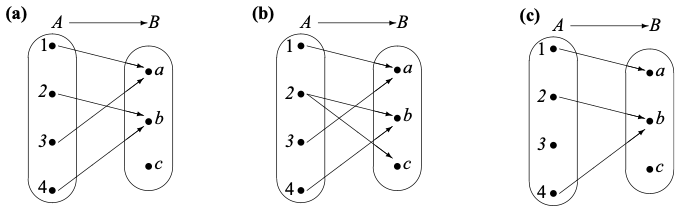
\includegraphics[width=\linewidth]{./img/arrow-diagrams.png}
\end{image}%
\end{exploration}%
\end{subsubsectionptx}
\end{subsectionptx}
%
%
\typeout{************************************************}
\typeout{Subsection 4.1.2 Today's Screencast}
\typeout{************************************************}
%
\begin{subsectionptx}{Today's Screencast}{}{Today's Screencast}{}{}{g:subsection:idm233531570800}
\begin{insight}{}{g:insight:idm233531570320}%
\setlength{\qrsize}{9em}
\setlength{\previewwidth}{\linewidth}
\addtolength{\previewwidth}{-\qrsize}
\begin{tcbraster}[raster columns=2, raster column skip=1pt, raster halign=center, raster force size=false, raster left skip=0pt, raster right skip=0pt]%
\begin{tcolorbox}[previewstyle, width=\previewwidth]%
\mono{No preview image available}%
\end{tcolorbox}%
\begin{tcolorbox}[qrstyle]%
[QR LINK]\end{tcolorbox}%
\end{tcbraster}%
\end{insight}
\end{subsectionptx}
%
%
\typeout{************************************************}
\typeout{Subsection 4.1.3 If you missed class today}
\typeout{************************************************}
%
\begin{subsectionptx}{If you missed class today}{}{If you missed class today}{}{}{g:subsection:idm233531569856}
%
\begin{enumerate}
\item{}Work through today's outline and read the marked pages in the book.%
\item{}Watch the screencast above.%
\item{}Submit any homework\slash{}assignments due today (check our \href{https://dordt.instructure.com/courses/3110050}{Canvas course} or the \href{https://prof.mkjanssen.org/ds/index.html\#schedule}{syllabus schedule} to see what's due).%
\item{}\href{mailto:mike.janssen@dordt.edu}{Send Dr. Janssen an email} or \href{https://calendly.com/mkjanssen/student-hours}{set up a student hours appointment} if you have any questions!%
\end{enumerate}
\end{subsectionptx}
\end{sectionptx}
%
%
\typeout{************************************************}
\typeout{Section 4.2 Feb. 3: Functions and Reading Discussion}
\typeout{************************************************}
%
\begin{sectionptx}{Feb. 3: Functions and Reading Discussion}{}{Feb. 3: Functions and Reading Discussion}{}{}{x:section:Feb-03}
\begin{introduction}{}%
\begin{assemblage}{Motivating Questions.}{g:assemblage:idm233531564640}%
Here are some questions we'll consider. %
\begin{enumerate}
\item{}How can we define functions recursively?%
\item{}What are injections, surjections, and bijections? How do we tell if a given function satisfies those extra condition(s)?%
\item{}What reactions do you have to the first part of M4HF?%
\end{enumerate}
%
\end{assemblage}
\end{introduction}%
%
%
\typeout{************************************************}
\typeout{Subsection 4.2.1 Outline}
\typeout{************************************************}
%
\begin{subsectionptx}{Outline}{}{Outline}{}{}{g:subsection:idm233531562032}
Today's material comes from \href{http://discrete.openmathbooks.org/dmoi3/sec_intro-functions.html}{Section 0.4} of the book. You're encouraged to read it before coming to class. We'll also discuss the first five chapters of \emph{Mathematics for Human Flourishing} following on the reading and reflection you recently completed, so please refresh your thoughts on that book as well.%
%
%
\typeout{************************************************}
\typeout{Subsubsection 4.2.1.1 Reading Discussion}
\typeout{************************************************}
%
\begin{subsubsectionptx}{Reading Discussion}{}{Reading Discussion}{}{}{g:subsubsection:idm233531560128}
\begin{principle}{}{}{g:principle:idm233531559664}%
We'll let the discussion take us where it may, but here are some suggested talking points to get started.%
%
\begin{itemize}[label=\textbullet]
\item{}What is matheamtics? What connection do you see between doing mathematics and being human?%
\item{}Think of a time you were captivated by exploring something. What analogies can you draw between doing math and doing this exploration?%
\item{}How does abstraction enrich the meaning of an idea? Give an example from your own experiences.%
\item{}Think of an activity you associate with play. Make a list of all the things you enjoy about its playful aspects. Does your list have analogies in mathematical activities?%
\item{}What role does beauty have in the Christian life?%
\item{}Where is mathematical beauty found in the world?%
\end{itemize}
\end{principle}
\end{subsubsectionptx}
%
%
\typeout{************************************************}
\typeout{Subsubsection 4.2.1.2 More Function Examples}
\typeout{************************************************}
%
\begin{subsubsectionptx}{More Function Examples}{}{More Function Examples}{}{}{g:subsubsection:idm233531556496}
\begin{exploration}{}{x:exploration:expl-birthday-function}%
Let \(b\) be the function that assigns to each person his or her birthday (month and day).%
%
\begin{enumerate}
\item{}Explain why \(b\) really is a function. We'll call it the \terminology{birthday function}.  What are the domain and codomain of \(b\)?%
\item{}What is \(\ran(b)\)?%
\item{}\href{https://en.wikipedia.org/wiki/Emmy_Noether}{Emmy Noether} was one of the founders of abstract algebra, and also made significant contributions to mathematical physics via her discovery of \href{https://en.wikipedia.org/wiki/Noether\%27s_theorem}{Noether's Theorem}. Her birthday was March 23, 1882. Translate this into a function statement, i.e.,%
\begin{equation*}
b(??) = ??
\end{equation*}
%
\item{}Is the following statement true or false? Explain. \begin{quote}%
For each day \(D\) of the year, there exists a person \(x\) such that \(b(x)=D\).\end{quote}
%
\item{}Is the following statement true or false? Explain. \begin{quote}%
For any people \(x\) and \(y\), if \(x\) and \(y\) are different people, then \(b(x) \ne b(y)\).\end{quote}
%
\end{enumerate}
\end{exploration}%
\begin{exploration}{}{x:exploration:expl-sum-of-divisors-function}%
Let \(\sigma\) be the function that associates to each positive natural number the sum of its distinct natural number divisors. This is called the \terminology{sum of the divisors function}. For example, the natural number divisors of 6 are 1, 2, 3, and 6. Thus:%
\begin{equation*}
\sigma(6) = 1  + 2 + 3 +6 = 12.
\end{equation*}
%
%
\begin{enumerate}
\item{}Calculate \(\sigma(k)\) for \(k = 1, 2, \ldots, 10\).%
\item{}Does there exist a natural number \(n\) such that \(\sigma(n) = 5\)? Justify your conclusion.%
\item{}Is it possible to find two different natural numbers \(m \ne n\) such that \(\sigma(m) = \sigma(n)\)? Explain.%
\end{enumerate}
\end{exploration}%
\end{subsubsectionptx}
%
%
\typeout{************************************************}
\typeout{Subsubsection 4.2.1.3 Injective and Surjective Functions}
\typeout{************************************************}
%
\begin{subsubsectionptx}{Injective and Surjective Functions}{}{Injective and Surjective Functions}{}{}{g:subsubsection:idm233531538832}
Two important properties functions \emph{may} possess are that of \emph{injectivity} and \emph{surjectivity}.%
\begin{assemblage}{Injective, Surjective, and Bijective Functions.}{p:assemblage:GUJ}%
A function is \terminology{injective} provided every element of the codomain is the image of \emph{at most} one element from the domain. An injective function is often called an \terminology{injection}.%
\par
A function is \terminology{surjective} provided every element of the codomain is the image of \emph{at least} one element from the domain. A surjective function is often called a \terminology{surjection}.%
\par
A function that is both injective and surjective is called \terminology{bijective}, and referred to as a \terminology{bijection}.%
\end{assemblage}
\end{subsubsectionptx}
\end{subsectionptx}
%
%
\typeout{************************************************}
\typeout{Subsection 4.2.2 Today's Screencast}
\typeout{************************************************}
%
\begin{subsectionptx}{Today's Screencast}{}{Today's Screencast}{}{}{g:subsection:idm233531531344}
\begin{insight}{}{g:insight:idm233531530864}%
\setlength{\qrsize}{9em}
\setlength{\previewwidth}{\linewidth}
\addtolength{\previewwidth}{-\qrsize}
\begin{tcbraster}[raster columns=2, raster column skip=1pt, raster halign=center, raster force size=false, raster left skip=0pt, raster right skip=0pt]%
\begin{tcolorbox}[previewstyle, width=\previewwidth]%
\mono{No preview image available}%
\end{tcolorbox}%
\begin{tcolorbox}[qrstyle]%
[QR LINK]\end{tcolorbox}%
\end{tcbraster}%
\end{insight}
\end{subsectionptx}
%
%
\typeout{************************************************}
\typeout{Subsection 4.2.3 If you missed class today}
\typeout{************************************************}
%
\begin{subsectionptx}{If you missed class today}{}{If you missed class today}{}{}{g:subsection:idm233531530400}
%
\begin{enumerate}
\item{}Work through today's outline and read the marked pages in the book.%
\item{}Watch the screencast above.%
\item{}Submit any homework\slash{}assignments due today (check our \href{https://dordt.instructure.com/courses/3110050}{Canvas course} or the \href{https://prof.mkjanssen.org/ds/index.html\#schedule}{syllabus schedule} to see what's due).%
\item{}\href{mailto:mike.janssen@dordt.edu}{Send Dr. Janssen an email} or \href{https://calendly.com/mkjanssen/student-hours}{set up a student hours appointment} if you have any questions!%
\end{enumerate}
\end{subsectionptx}
\end{sectionptx}
%
%
\typeout{************************************************}
\typeout{Section 4.3 Feb. 5: Functions}
\typeout{************************************************}
%
\begin{sectionptx}{Feb. 5: Functions}{}{Feb. 5: Functions}{}{}{x:section:Feb-05}
\begin{introduction}{}%
\begin{assemblage}{Motivating Questions.}{g:assemblage:idm233531525264}%
Here are some questions we'll consider. %
\begin{enumerate}
\item{}What is the image of an element\slash{}set under a function?%
\item{}What is the complete inverse image of an element in the codomain of a function?%
\item{}What is the inverse image of the subset of the codomain of a function?%
\end{enumerate}
%
\end{assemblage}
\end{introduction}%
%
%
\typeout{************************************************}
\typeout{Subsection 4.3.1 Outline}
\typeout{************************************************}
%
\begin{subsectionptx}{Outline}{}{Outline}{}{}{g:subsection:idm233531522784}
Today's material comes from the last part of \href{http://discrete.openmathbooks.org/dmoi3/sec_intro-functions.html}{Section 0.4} of the book. You're encouraged to read it before coming to class.%
%
%
\typeout{************************************************}
\typeout{Subsection 4.3.1.1 More on Injections, Surjections, and Bijections}
\typeout{************************************************}
%
\begin{subsectionptx}{More on Injections, Surjections, and Bijections}{}{More on Injections, Surjections, and Bijections}{}{}{g:subsection:idm233531521376}
\begin{exploration}{}{x:exploration:expl-fcn-injsurjbij}%
Consider the functions below. Are they injective, surjective, neither, or bijective? Explain.%
%
\begin{enumerate}
\item{}\(f: \N\to \N\) given by the rule \(f(n) = 2n\).%
\item{}\(f: \N\to \set{0,2,4,6,\ldots}\) given by the rule \(f(n) = 2n\).%
\item{}\(f: \set{1,2,3,4,5}\to \set{1,2,3,4}\) given by the \terminology{two-line notation}%
\begin{equation*}
f = \begin{pmatrix}1 \amp 2 \amp 3 \amp 4 \amp 5 \\ 2 \amp 1 \amp 3 \amp 1\amp 4 \end{pmatrix},
\end{equation*}
where the number in the first row is understood to map to the number below it.%
\item{}The birthday function described in \hyperref[x:exploration:expl-birthday-function]{Exploration~{\xreffont\ref{x:exploration:expl-birthday-function}}}.%
\item{}The sum of divisors function described in \hyperref[x:exploration:expl-sum-of-divisors-function]{Exploration~{\xreffont\ref{x:exploration:expl-sum-of-divisors-function}}}.%
\item{}The function \(f : \N\to\Z\) given by%
\begin{equation*}
f(n) = \begin{cases} n/2 \amp \text{ if } n \text{ is even} \\ -(n+1)/2 \amp \text{ if } n \text{ is odd}\end{cases}.
\end{equation*}
%
\end{enumerate}
\end{exploration}%
\begin{exploration}{A very discrete math question.}{x:exploration:expl-first-counting}%
Using the two-line notation described above, write out all functions \(f: \set{1,2,3}\to \set{a,b}\).%
%
\begin{enumerate}
\item{}How many such functions are there?%
\item{}How many are injective?%
\item{}How many are surjective?%
\item{}How many are bijective?%
\end{enumerate}
\end{exploration}%
\end{subsectionptx}
%
%
\typeout{************************************************}
\typeout{Subsubsection 4.3.1.1 Recursive Definitions of Functions}
\typeout{************************************************}
%
\begin{subsubsectionptx}{Recursive Definitions of Functions}{}{Recursive Definitions of Functions}{}{}{g:subsubsection:idm233531509696}
We've so far seen that we can define functions by listing ordered pairs, giving rules, drawing arrow diagrams, and the like. Another important method for defining functions (especially in computer science) is with a \terminology{recursive definition}.%
\par
Recursively defined functions are often easier to create from a ``real world'' problem, because they describe how the values of the functions are changing. However, this comes with a price. It is harder to calculate the image of a single input, since you need to know the images of other (previous) elements in the domain.%
\begin{assemblage}{Recursively Defined Functions.}{p:assemblage:aNA}%
\index{initial condition!for a function}\index{recurrence relation!for a function} For a function \(f:\N \to \N\), a \terminology{recursive definition} consists of an \terminology{initial condition} together with a \terminology{recurrence relation}. The initial condition is the explicitly given value of \(f(0)\). The recurrence relation is a formula for \(f(n+1)\) in terms for \(f(n)\) (and possibly \(n\) itself).%
\end{assemblage}
\begin{exploration}{}{g:exploration:idm233531505872}%
Consider the recurrence \(f : \N\to\N\) given by \(f(n+1) = 3f(n)\). Note that this is not enough to define a function since we don't have an initial condition. For each initial condition below, find the value of \(f(4)\).%
%
\begin{enumerate}
\item{}\(\displaystyle f(0)=0\)%
\item{}\(\displaystyle f(0)=1\)%
\item{}\(\displaystyle f(0)=2\)%
\item{}\(\displaystyle f(0)=100\)%
\end{enumerate}
\end{exploration}%
\end{subsubsectionptx}
%
%
\typeout{************************************************}
\typeout{Subsubsection 4.3.1.2 Image}
\typeout{************************************************}
%
\begin{subsubsectionptx}{Image}{}{Image}{}{}{g:subsubsection:idm233531496320}
Let \(f : X\to Y\) be a function. The \terminology{image of \(x\in X\) under \(f\)} is the value \(y\in Y\) for which \(f(x) = y\). This extends to entire subsets of the domain. Given \(A\subseteq X\), the \terminology{image of \(A\) under \(f\)} is the set%
\begin{equation*}
f(A) = \setof{f(x)}{x\in A}.
\end{equation*}
%
\begin{exploration}{}{x:exploration:expl-image-of-set}%
Consider the function \(f : \N\times\N \to \N\) given by \(f((a,b)) = a+b\). Given \(A = \setof{(a,b)\in \N\times\N}{a,b\le 10}\), find (with justification) \(f(A)\).%
\end{exploration}%
\begin{example}{}{g:example:idm233531488752}%
Suppose \(f : X\to Y\) and \(A,B\subseteq X\). Is it true that \(f(A\cup B) = f(A)\cup f(B)\)?%
\end{example}
\end{subsubsectionptx}
%
%
\typeout{************************************************}
\typeout{Subsubsection 4.3.1.3 Inverse Images (Preimages)}
\typeout{************************************************}
%
\begin{subsubsectionptx}{Inverse Images (Preimages)}{}{Inverse Images (Preimages)}{}{}{g:subsubsection:idm233531488496}
If images tell us where functions send elements and sets of the codomain, then \terminology{inverse images} (sometimes called \emph{preimages}) describe which objects in the domain get sent to particular objects (elements, subsets) of the codomain. \begin{aside}{}{g:aside:idm233531485200}%
\end{aside}
%
\par
Given a subset \(B\subseteq Y\), the \terminology{inverse image of \(B\) under \(f\)} the set%
\begin{equation*}
f^{-1}(B) = \setof{x\in X}{f(x)\in B}.
\end{equation*}
If \(B = \set{y}\) for some \(y\in Y\), we often write \(f^{-1}(\set{y})\) as \(f^{-1}(y)\); it is the \terminology{complete inverse image of \(y\) under \(f\)} (but again, \(f^{-1}\) need not be a well-defined function).%
\begin{exploration}{}{g:exploration:idm233564809680}%
Consider again the function from \hyperref[x:exploration:expl-image-of-set]{Exploration~{\xreffont\ref{x:exploration:expl-image-of-set}}}.%
%
\begin{enumerate}
\item{}Find \(f^{-1}(3)\) and \(f^{-1}(\set{0,1,2,3})\).%
\item{}Give geometric descriptions of \(f^{-1}(n)\) and \(f^{-1}(\set{0,1,2,\ldots,n})\) for any \(n\ge 1\).%
\item{}Calculate \(|f^{-1}(8)\) and \(|f^{-1}(\set{0,1,\ldots,8})\).%
\end{enumerate}
\end{exploration}%
\begin{question}{}{g:question:idm233564804288}%
Suppose \(f : X\to Y\) is a function and \(1\in Y\). What can you say about \(f^{-1}(1)\) if you that:%
%
\begin{enumerate}
\item{}\(f\) is injective? Explain.%
\item{}\(f\) is surjective? Explain.%
\item{}\(f\) is bijective? Explain.%
\end{enumerate}
\end{question}
\begin{assemblage}{Challenge.}{g:assemblage:idm233564800640}%
Let \(f: X\to Y\) be a function with \(A\subseteq X\) and \(B\subseteq Y\). %
\begin{enumerate}
\item{}Is \(f^{-1}(f(A))=A\)? Always? Sometimes? Never? Explain.%
\item{}Is \(f(f^{-1}(B)) = B\)? Always? Sometimes? Never? Explain.%
\item{}If one or both of the above do not always hold, is there something else you can say? Will equality always hold for particular types of functions? Is there some other relationship other than equality that would always hold? Explore.%
\end{enumerate}
 As you consider the statements above, you may want to build one or two representative examples to test. But be careful! If your examples are too similar, you may be led down an erroneous path.%
\end{assemblage}
\end{subsubsectionptx}
\end{subsectionptx}
%
%
\typeout{************************************************}
\typeout{Subsection 4.3.2 Today's Screencast}
\typeout{************************************************}
%
\begin{subsectionptx}{Today's Screencast}{}{Today's Screencast}{}{}{g:subsection:idm233564795776}
\begin{insight}{}{g:insight:idm233564795392}%
\setlength{\qrsize}{9em}
\setlength{\previewwidth}{\linewidth}
\addtolength{\previewwidth}{-\qrsize}
\begin{tcbraster}[raster columns=2, raster column skip=1pt, raster halign=center, raster force size=false, raster left skip=0pt, raster right skip=0pt]%
\begin{tcolorbox}[previewstyle, width=\previewwidth]%
\mono{No preview image available}%
\end{tcolorbox}%
\begin{tcolorbox}[qrstyle]%
[QR LINK]\end{tcolorbox}%
\end{tcbraster}%
\end{insight}
\end{subsectionptx}
%
%
\typeout{************************************************}
\typeout{Subsection 4.3.3 If you missed class today}
\typeout{************************************************}
%
\begin{subsectionptx}{If you missed class today}{}{If you missed class today}{}{}{g:subsection:idm233564795008}
%
\begin{enumerate}
\item{}Work through today's outline and read the marked pages in the book.%
\item{}Watch the screencast above.%
\item{}Submit any homework\slash{}assignments due today (check our \href{https://dordt.instructure.com/courses/3110050}{Canvas course} or the \href{https://prof.mkjanssen.org/ds/index.html\#schedule}{syllabus schedule} to see what's due).%
\item{}\href{mailto:mike.janssen@dordt.edu}{Send Dr. Janssen an email} or \href{https://calendly.com/mkjanssen/student-hours}{set up a student hours appointment} if you have any questions!%
\end{enumerate}
\end{subsectionptx}
\end{sectionptx}
\end{chapterptx}
%
%
\typeout{************************************************}
\typeout{Chapter 5 Week 5: Feb. 8-12}
\typeout{************************************************}
%
\begin{chapterptx}{Week 5: Feb. 8-12}{}{Week 5: Feb. 8-12}{}{}{x:chapter:Week-05}
\begin{introduction}{}%
This week, we investigate some counting problems with intentionality. We'll develop some principles for doing certain types of counting, and then see how far we can push them.%
\par
Your second portfolio problem is due February 17 (next week Wednesday), so be sure to be working on that after it's assigned this week. Also, you should be working on revising your first portfolio problem based on the written comments on the submitted PDF.%
\end{introduction}%
%
%
\typeout{************************************************}
\typeout{Section 5.1 Feb. 8: The Additive and Multiplicative Principles}
\typeout{************************************************}
%
\begin{sectionptx}{Feb. 8: The Additive and Multiplicative Principles}{}{Feb. 8: The Additive and Multiplicative Principles}{}{}{x:section:Feb-08}
\begin{introduction}{}%
\begin{assemblage}{Motivating Questions.}{g:assemblage:idm233564787696}%
Here are some questions we'll consider. %
\begin{enumerate}
\item{}What are \terminology{counting problems}?%
\item{}What principles can we develop to explore introductory counting problems?%
\item{}(If time): How can we use the language of sets to aid in counting?%
\end{enumerate}
%
\end{assemblage}
\end{introduction}%
%
%
\typeout{************************************************}
\typeout{Subsection 5.1.1 Outline}
\typeout{************************************************}
%
\begin{subsectionptx}{Outline}{}{Outline}{}{}{g:subsection:idm233564784704}
Today's material comes from \href{http://discrete.openmathbooks.org/dmoi3/sec_counting-addmult.html}{the first part of Section 1.1} of the book. You're encouraged to read it before coming to class.%
%
%
\typeout{************************************************}
\typeout{Subsubsection 5.1.1.1 First Principles}
\typeout{************************************************}
%
\begin{subsubsectionptx}{First Principles}{}{First Principles}{}{}{g:subsubsection:idm233564783504}
Today we start counting. Well, you've been doing a form of counting your whole life, and we saw an initial example of the types of counting questions in which we'll be interested in \hyperref[x:exploration:expl-first-counting]{Exploration~{\xreffont\ref{x:exploration:expl-first-counting}}}. Our counting questions will often take the form ``How many possible \emph{qrsabs} are there subject to the constraint \emph{jkasdghjkl}, where the order of the \emph{qrsabs} may\slash{}may not matter?'' (And where these words are mostly made up).%
\par
Consider the following investigation from our book.%
\begin{investigation}{}{p:investigation:wnA}%
%
\begin{enumerate}
\item{}A restaurant offers 8 appetizers and 14 entrées. How many choices do you have if:%
\begin{enumerate}
\item{}you will eat one dish, either an appetizer or an entrée?%
\item{}you are extra hungry and want to eat both an appetizer and an entrée?%
\end{enumerate}
%
\item{}Think about the methods you used to solve question 1. Write down the rules for these methods.%
\item{}Do your rules work? A standard deck of playing cards has 26 red cards and 12 face cards.%
\begin{enumerate}
\item{}How many ways can you select a card which is either red or a face card?%
\item{}How many ways can you select a card which is both red and a face card?%
\item{}How many ways can you select two cards so that the first one is red and the second one is a face card?%
\end{enumerate}
%
\end{enumerate}
%
\end{investigation}%
This investigation suggests the following principle.%
\begin{assemblage}{Additive Principle.}{x:assemblage:additive-principle}%
The \terminology{additive principle} states that if event \(A\) can occur in \(m\) ways, and event \(B\) can occur in \(n\) \emph{disjoint} ways, then the event ``\(A\) or \(B\)'' can occur in \(m + n\) ways.%
\end{assemblage}
\begin{question}{}{g:question:idm233531483296}%
What does the word \terminology{disjoint} mean in the context of the additive principle? What if we have three different events?%
\end{question}
\end{subsubsectionptx}
%
%
\typeout{************************************************}
\typeout{Subsubsection 5.1.1.2 The Multiplicative Principle}
\typeout{************************************************}
%
\begin{subsubsectionptx}{The Multiplicative Principle}{}{The Multiplicative Principle}{}{}{g:subsubsection:idm233531482288}
Let's consider the following investigation.%
\begin{investigation}{}{x:investigation:invest-pizzas}%
Prof. Clark is getting ready to order pizzas for the next Pizza and Presentation. Suppose there are:%
%
\begin{itemize}[label=\textbullet]
\item{}Three choices for crusts (thin, hand-tossed, thick)%
\item{}Three choices for sauce (red, white, BBQ)%
\item{}Fifteen choices for toppings%
\end{itemize}
%
\begin{enumerate}
\item{}How many different pizzas are possible if Prof. Clark insists on a thin crust with red sauce and one topping?%
\item{}Suppose now that, while insisting on thin crust and a single topping, Prof. Clark is considering any choice of sauce. How many different such pizzas are possible?%
\item{}Explain why your answer to the previous question makes sense in terms of the addition principle above. Is there another general rule or principle that we can articulate?%
\item{}Given your answer to the previous question, how many different single-topping pizzas could Prof. Clark order? How many two-topping pizzas could he order?%
\end{enumerate}
\end{investigation}%
\begin{assemblage}{Multiplicative Principle.}{x:assemblage:multiplicative-principle}%
The \terminology{multiplicative principle} states that if event \(A\) can occur in \(m\) ways, and each possibility for \(A\) allows for exactly \(n\) ways for event \(B\), then the event ``\(A\) and \(B\)'' can occur in \(m \cdot n\) ways.%
\end{assemblage}
\begin{exploration}{}{g:exploration:idm233528790288}%
We usually write numbers in decimal form (or base 10), meaning numbers are composed using 10 different ``digits'' \(\{0,1,\ldots, 9\}\). Sometimes though it is useful to write numbers \terminology{hexadecimal} or base 16. Now there are 16 distinct digits that can be used to form numbers: \(\{0, 1, \ldots, 9, \mathrm{A, B, C, D, E, F}\}\). So for example, a 3 digit hexadecimal number might be 2B8.%
\begin{enumerate}
\item{}How many 2-digit hexadecimals are there in which the first digit is E or F? Explain your answer in terms of the additive principle (using either events or sets).%
\par
%
\item{}Explain why your answer to the previous part is correct in terms of the multiplicative principle (using either events or sets). Why do both the additive and multiplicative principles give you the same answer?%
\item{}How many 3-digit hexadecimals start with a letter (A-F) and end with a numeral (0-9)? Explain.%
\par
%
\item{}How many 3-digit hexadecimals start with a letter (A-F) or end with a numeral (0-9) (or both)? Explain.%
\par
%
\end{enumerate}
%
\end{exploration}%
\end{subsubsectionptx}
%
%
\typeout{************************************************}
\typeout{Subsubsection 5.1.1.3 Counting with Sets}
\typeout{************************************************}
%
\begin{subsubsectionptx}{Counting with Sets}{}{Counting with Sets}{}{}{g:subsubsection:idm233531466752}
One of our uses for the language of set theory we developed a few weeks ago is to make our counting arguments unambiguous and rigorous.%
\begin{assemblage}{Additive Principle (with sets).}{p:assemblage:leB}%
Given two sets \(A\) and \(B\), if \(A \cap B = \emptyset\) (that is, if there is no element in common to both \(A\) and \(B\)), then%
\begin{equation*}
\card{A \cup B} = \card{A} + \card{B}\text{.}
\end{equation*}
%
\end{assemblage}
Similarly, we obtain a set-theoretic version of the multiplicative principle.%
\begin{assemblage}{Multiplicative Principle (with sets).}{p:assemblage:xsT}%
Given two sets \(A\) and \(B\), we have \(\card{A \times B} = \card{A} \cdot \card{B}\).%
\end{assemblage}
\end{subsubsectionptx}
%
%
\typeout{************************************************}
\typeout{Subsubsection 5.1.1.4 Exploring PIE}
\typeout{************************************************}
%
\begin{subsubsectionptx}{Exploring PIE}{}{Exploring PIE}{}{}{g:subsubsection:idm233531454720}
We close today by thinking about the following question.%
\begin{question}{}{g:question:idm233531454112}%
Suppose Casey's Bakery produces some number of pies: 10 contain blueberries, and 15 contain peaches.%
%
\begin{enumerate}
\item{}What is the largest number of pies Casey's could have produced?%
\item{}What is the smallest number of pies Casey's could have produced?%
\item{}What information do we need in order to determine the precise number of pies that Casey's produced?%
\item{}Present your findings in terms of the cardinalities of certain sets.%
\end{enumerate}
\end{question}
\end{subsubsectionptx}
\end{subsectionptx}
%
%
\typeout{************************************************}
\typeout{Subsection 5.1.2 Today's Screencast}
\typeout{************************************************}
%
\begin{subsectionptx}{Today's Screencast}{}{Today's Screencast}{}{}{g:subsection:idm233531451680}
\begin{insight}{}{g:insight:idm233531451296}%
\setlength{\qrsize}{9em}
\setlength{\previewwidth}{\linewidth}
\addtolength{\previewwidth}{-\qrsize}
\begin{tcbraster}[raster columns=2, raster column skip=1pt, raster halign=center, raster force size=false, raster left skip=0pt, raster right skip=0pt]%
\begin{tcolorbox}[previewstyle, width=\previewwidth]%
\mono{No preview image available}%
\end{tcolorbox}%
\begin{tcolorbox}[qrstyle]%
[QR LINK]\end{tcolorbox}%
\end{tcbraster}%
\end{insight}
\end{subsectionptx}
%
%
\typeout{************************************************}
\typeout{Subsection 5.1.3 If you missed class today}
\typeout{************************************************}
%
\begin{subsectionptx}{If you missed class today}{}{If you missed class today}{}{}{g:subsection:idm233531450912}
%
\begin{enumerate}
\item{}Work through today's outline and read the marked pages in the book.%
\item{}Watch the screencast above.%
\item{}Submit any homework\slash{}assignments due today (check our \href{https://dordt.instructure.com/courses/3110050}{Canvas course} or the \href{https://prof.mkjanssen.org/ds/index.html\#schedule}{syllabus schedule} to see what's due).%
\item{}\href{mailto:mike.janssen@dordt.edu}{Send Dr. Janssen an email} or \href{https://calendly.com/mkjanssen/student-hours}{set up a student hours appointment} if you have any questions!%
\end{enumerate}
\end{subsectionptx}
\end{sectionptx}
%
%
\typeout{************************************************}
\typeout{Section 5.2 Feb. 10: More Counting with Sets and PIE}
\typeout{************************************************}
%
\begin{sectionptx}{Feb. 10: More Counting with Sets and PIE}{}{Feb. 10: More Counting with Sets and PIE}{}{}{x:section:Feb-10}
\begin{introduction}{}%
\begin{assemblage}{Motivating Questions.}{g:assemblage:idm233531445440}%
Here are some questions we'll consider. %
\begin{enumerate}
\item{}What is the Principle of Inclusion\slash{}Exclusion?%
\item{}How can we use PIE to count cardinalities of unions?%
\end{enumerate}
%
\end{assemblage}
\end{introduction}%
%
%
\typeout{************************************************}
\typeout{Subsection 5.2.1 Outline}
\typeout{************************************************}
%
\begin{subsectionptx}{Outline}{}{Outline}{}{}{g:subsection:idm233531445696}
Today's material comes from \href{http://discrete.openmathbooks.org/dmoi3/sec_counting-addmult.html}{Section 1.1} of the book. You're encouraged to read it before coming to class.%
%
%
\typeout{************************************************}
\typeout{Subsubsection 5.2.1.1 More PIE}
\typeout{************************************************}
%
\begin{subsubsectionptx}{More PIE}{}{More PIE}{}{}{g:subsubsection:idm233531442080}
\begin{investigation}{}{x:investigation:invest-village-inn}%
A recent buzz marketing campaign for \emph{Village Inn} surveyed patrons on their pie preferences. People were asked whether they enjoyed (A) Apple, (B) Blueberry or (C) Cherry pie (respondents answered yes or no to each type of pie, and could say yes to more than one type). The following table shows the results of the survey.%
\begin{sidebyside}{1}{0}{0}{0}%
\begin{sbspanel}{1}%
\resizebox{\linewidth}{!}{%
{\centering%
{\tabularfont%
\begin{tabular}{cccccccc}
\multicolumn{1}{rA}{Pies enjoyed:}&A&B&C&AB&AC&BC&ABC\tabularnewline\hrulethin
\multicolumn{1}{rA}{Number of people:}&20&13&26&9&15&7&5
\end{tabular}
}%
\par}
}%
\end{sbspanel}%
\end{sidebyside}%
\par
How many of those asked enjoy at least one of the kinds of pie? Also, explain why the answer is not 95.%
\end{investigation}%
\begin{question}{}{g:question:idm233531431824}%
What becomes of the additive principle when the sets are not disjoint? That is, can we precisely describe a formula for \(\card{A\cup B}\) if \(A\cap B\ne \emptyset\)?%
\end{question}
\begin{assemblage}{Cardinality of a union (2 sets).}{p:assemblage:dAc}%
For any finite sets \(A\) and \(B\),%
\begin{equation*}
\card{A \cup B} = \card{A} + \card{B} - \card{A \cap B}\text{.}
\end{equation*}
%
\end{assemblage}
Let's revisit \hyperref[x:investigation:invest-village-inn]{Investigation~{\xreffont\ref{x:investigation:invest-village-inn}}} to establish PIE for three sets.%
\begin{question}{}{g:question:idm233531425408}%
Given sets \(A, B, C\), can we construct a formula for \(\card{A\cup B\cup C}\)?%
\end{question}
\begin{assemblage}{Cardinality of a union (3 sets).}{p:assemblage:JHl}%
For any finite sets \(A\), \(B\), and \(C\),%
\begin{equation*}
\card{A \cup B \cup C} = \card{A} + \card{B} + \card{C} - \card{A \cap B} - \card{A \cap C} - \card{B \cap C} + \card{A \cap B \cap C}\text{.}
\end{equation*}
%
\end{assemblage}
To determine how many elements are in at least one of \(A\), \(B\), or \(C\) we add up all the elements in each of those sets. However, when we do that, any element in both \(A\) and \(B\) is counted twice. Also, each element in both \(A\) and \(C\) is counted twice, as are elements in \(B\) and \(C\), so we take each of those out of our sum once. But now what about the elements which are in \(A \cap B \cap C\) (in all three sets)? We added them in three times, but also removed them three times. They have not yet been counted. Thus we add those elements back in at the end.%
\par
This process of adding in, then taking out, then adding back in, and so on is called the \emph{Principle of Inclusion\slash{}Exclusion}, or simply PIE. We will return to this counting technique later to solve for more complicated problems (involving more than 3 sets).%
\end{subsubsectionptx}
%
%
\typeout{************************************************}
\typeout{Subsubsection 5.2.1.2 Counting Subsets}
\typeout{************************************************}
%
\begin{subsubsectionptx}{Counting Subsets}{}{Counting Subsets}{}{}{g:subsubsection:idm233531411760}
Here's another counting problem involving sets. Given a set \(A\), recall that the \emph{power set of} \(A\), denoted \(\pow(A)\), is the set of all subsets of \(A\). Can we predict ahead of time how many subsets a set will have? That is, given a set \(A\), can we calculate \(\card{\pow(A)}\) if we know \(\card{A}\)?%
\begin{exploration}{}{g:exploration:idm233531411152}%
Consider the family of sets \(X_n = \set{1,2,\ldots,n}\) for \(n\ge 1\).%
%
\begin{enumerate}
\item{}Explicitly calculate \(\card{\pow(X_n)}\) for \(1 \le n \le 3\).%
\item{}What do you think \(\card{\pow(X_4)}\) will be? Either make an argument or explicitly verify your guess.%
\item{}If you write a number in binary, you only use 0's and 1's (which in this context are called \emph{binary digits}, or \terminology{bits}. We'll call a string of 0's and 1's a \terminology{bit-string}. Examples of bit-strings are things like 0101, 011100111, etc. How many bit-strings of length 4 are there?%
\item{}What do the previous two questions have to do with one another?%
\item{}Make a conjecture for \(\card{\pow(X_n)}\) in terms of \(n\).%
\end{enumerate}
\end{exploration}%
\end{subsubsectionptx}
\end{subsectionptx}
%
%
\typeout{************************************************}
\typeout{Subsection 5.2.2 Today's Screencast}
\typeout{************************************************}
%
\begin{subsectionptx}{Today's Screencast}{}{Today's Screencast}{}{}{g:subsection:idm233531400384}
\begin{insight}{}{g:insight:idm233531400128}%
\setlength{\qrsize}{9em}
\setlength{\previewwidth}{\linewidth}
\addtolength{\previewwidth}{-\qrsize}
\begin{tcbraster}[raster columns=2, raster column skip=1pt, raster halign=center, raster force size=false, raster left skip=0pt, raster right skip=0pt]%
\begin{tcolorbox}[previewstyle, width=\previewwidth]%
\mono{No preview image available}%
\end{tcolorbox}%
\begin{tcolorbox}[qrstyle]%
[QR LINK]\end{tcolorbox}%
\end{tcbraster}%
\end{insight}
\end{subsectionptx}
%
%
\typeout{************************************************}
\typeout{Subsection 5.2.3 If you missed class today}
\typeout{************************************************}
%
\begin{subsectionptx}{If you missed class today}{}{If you missed class today}{}{}{g:subsection:idm233531399648}
%
\begin{enumerate}
\item{}Work through today's outline and read the marked pages in the book.%
\item{}Watch the screencast above.%
\item{}Submit any homework\slash{}assignments due today (check our \href{https://dordt.instructure.com/courses/3110050}{Canvas course} or the \href{https://prof.mkjanssen.org/ds/index.html\#schedule}{syllabus schedule} to see what's due).%
\item{}\href{mailto:mike.janssen@dordt.edu}{Send Dr. Janssen an email} or \href{https://calendly.com/mkjanssen/student-hours}{set up a student hours appointment} if you have any questions!%
\end{enumerate}
\end{subsectionptx}
\end{sectionptx}
%
%
\typeout{************************************************}
\typeout{Section 5.3 Feb. 12: Binomial Coefficients I}
\typeout{************************************************}
%
\begin{sectionptx}{Feb. 12: Binomial Coefficients I}{}{Feb. 12: Binomial Coefficients I}{}{}{x:section:Feb-12}
\begin{introduction}{}%
\begin{assemblage}{Motivating Questions.}{g:assemblage:idm233531394528}%
Here are some questions we'll consider. %
\begin{enumerate}
\item{}How can we count chess rook moves?%
\item{}How can we count subsets of a set?%
\item{}How can we count lattice paths?%
\item{}How can we calculate binomial coefficients?%
\item{}How are these questions related?%
\end{enumerate}
%
\end{assemblage}
\end{introduction}%
%
%
\typeout{************************************************}
\typeout{Subsection 5.3.1 Outline}
\typeout{************************************************}
%
\begin{subsectionptx}{Outline}{}{Outline}{}{}{g:subsection:idm233531391600}
Today's material comes from \href{http://discrete.openmathbooks.org/dmoi3/sec_counting-binom.html}{Section 1.2} of the book. You're encouraged to read it before coming to class.%
%
%
\typeout{************************************************}
\typeout{Subsubsection 5.3.1.1 Counting Rook Paths}
\typeout{************************************************}
%
\begin{subsubsectionptx}{Counting Rook Paths}{}{Counting Rook Paths}{}{}{g:subsubsection:idm233531390256}
\begin{investigation}{}{p:investigation:qkg}%
\index{rook paths}%
\index{chessboard!rook paths}%
\index{rook paths}%
\index{chessboard!rook paths}%
In chess, a rook can move only in straight lines (not diagonally). Fill in each square of the chess board below with the number of different shortest paths the rook, in the upper left corner, can take to get to that square. For example, one square is already filled in. There are six different paths from the rook to the square: DDRR (down down right right), DRDR, DRRD, RDDR, RDRD and RRDD.%
\begin{sidebyside}{1}{0.25}{0.25}{0}%
\begin{sbspanel}{0.5}%
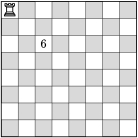
\includegraphics[width=\linewidth]{./img/chessboard.svg}
\end{sbspanel}%
\end{sidebyside}%
\end{investigation}%
\end{subsubsectionptx}
%
%
\typeout{************************************************}
\typeout{Subsubsection 5.3.1.2 Counting Subsets and Bit Strings}
\typeout{************************************************}
%
\begin{subsubsectionptx}{Counting Subsets and Bit Strings}{}{Counting Subsets and Bit Strings}{}{}{g:subsubsection:idm233531384880}
\begin{exploration}{}{g:exploration:idm233531384400}%
Consider the set \(A=\set{1,2,3,4,5,6}\). How many subsets does \(A\) have? How many of those subsets contain exactly four elements? Exactly three?%
\end{exploration}%
\begin{exploration}{}{g:exploration:idm233531382592}%
Let's consider bit strings of length 6. We'll denote the set of such strings as \(\mathbf{B}^6\). Further, define the \terminology{weight} of a bit string as the number of 1's in the string (equivalently, the sum of the bits in the string). We'll denote the set of \(n\)-bit strings with weight \(k\) by \(\mathbf{B}^n_k\).%
%
\begin{enumerate}
\item{}How many weight four bit strings are there? That is, what is \(\card{\mathbf{B}^6_4}\)?%
\item{}Calculate \(\card{\mathbf{B}^6_3}\) and \(\card{\mathbf{B}^6_2}\).%
\item{}How are these questions related to the subset question?%
\end{enumerate}
\end{exploration}%
Note that we've used the \hyperref[x:assemblage:additive-principle]{additive principle} with a \terminology{recurrence relation}.%
\end{subsubsectionptx}
%
%
\typeout{************************************************}
\typeout{Subsubsection 5.3.1.3 Lattice Paths}
\typeout{************************************************}
%
\begin{subsubsectionptx}{Lattice Paths}{}{Lattice Paths}{}{}{g:subsubsection:idm233528213648}
\index{integer lattice}\index{lattice, integer|see{integer lattice}} The \terminology{integer lattice} is the set of all points in the Cartesian plane for which both the \(x\) and \(y\) coordinates are integers. If you like to draw graphs on graph paper, the lattice is the set of all the intersections of the grid lines.%
\par
A \terminology{lattice path} \index{lattice path} is one of the shortest possible paths connecting two points on the lattice, moving only horizontally and vertically. For example, here are three possible lattice paths from the point \((0,0)\) to \((3,2)\):%
\begin{sidebyside}{3}{0.0166666666666667}{0.0166666666666667}{0.0333333333333333}%
\begin{sbspanel}{0.3}%
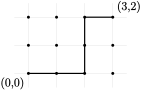
\includegraphics[width=\linewidth]{./img/lattice-path-1.svg}
\end{sbspanel}%
\begin{sbspanel}{0.3}%
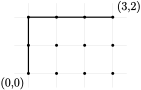
\includegraphics[width=\linewidth]{./img/lattice-path-2.svg}
\end{sbspanel}%
\begin{sbspanel}{0.3}%
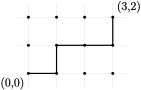
\includegraphics[width=\linewidth]{./img/lattice-path-3.svg}
\end{sbspanel}%
\end{sidebyside}%
\begin{exploration}{}{g:exploration:idm233528203872}%
How many lattice paths are there from \((0,0)\) to \((3,2)\)? Again, how is this question related to the previous questions?%
\end{exploration}%
\end{subsubsectionptx}
\end{subsectionptx}
%
%
\typeout{************************************************}
\typeout{Subsection 5.3.2 Today's Screencast}
\typeout{************************************************}
%
\begin{subsectionptx}{Today's Screencast}{}{Today's Screencast}{}{}{g:subsection:idm233528204608}
\begin{insight}{}{g:insight:idm233528201936}%
\setlength{\qrsize}{9em}
\setlength{\previewwidth}{\linewidth}
\addtolength{\previewwidth}{-\qrsize}
\begin{tcbraster}[raster columns=2, raster column skip=1pt, raster halign=center, raster force size=false, raster left skip=0pt, raster right skip=0pt]%
\begin{tcolorbox}[previewstyle, width=\previewwidth]%
\mono{No preview image available}%
\end{tcolorbox}%
\begin{tcolorbox}[qrstyle]%
[QR LINK]\end{tcolorbox}%
\end{tcbraster}%
\end{insight}
\end{subsectionptx}
%
%
\typeout{************************************************}
\typeout{Subsection 5.3.3 If you missed class today}
\typeout{************************************************}
%
\begin{subsectionptx}{If you missed class today}{}{If you missed class today}{}{}{g:subsection:idm233528201392}
%
\begin{enumerate}
\item{}Work through today's outline and read the marked pages in the book.%
\item{}Watch the screencast above.%
\item{}Submit any homework\slash{}assignments due today (check our \href{https://dordt.instructure.com/courses/3110050}{Canvas course} or the \href{https://prof.mkjanssen.org/ds/index.html\#schedule}{syllabus schedule} to see what's due).%
\item{}\href{mailto:mike.janssen@dordt.edu}{Send Dr. Janssen an email} or \href{https://calendly.com/mkjanssen/student-hours}{set up a student hours appointment} if you have any questions!%
\end{enumerate}
\end{subsectionptx}
\end{sectionptx}
\end{chapterptx}
%
%
\typeout{************************************************}
\typeout{Chapter 6 Week 6: Feb. 15-19}
\typeout{************************************************}
%
\begin{chapterptx}{Week 6: Feb. 15-19}{}{Week 6: Feb. 15-19}{}{}{x:chapter:Week-06}
\begin{introduction}{}%
This week, we continue exploring elementary counting problems through our study of binomial coefficients and the related notions of permutations and combinations. Near the end of the week, we may see some combinatorial proofs (to be explored in greater detail next week). Also, the \href{}{second M4HF reflection} is due on Friday.%
\end{introduction}%
%
%
\typeout{************************************************}
\typeout{Section 6.1 Feb. 17: Bionomial Coefficients II}
\typeout{************************************************}
%
\begin{sectionptx}{Feb. 17: Bionomial Coefficients II}{}{Feb. 17: Bionomial Coefficients II}{}{}{x:section:Feb-17}
\begin{introduction}{}%
\begin{assemblage}{Motivating Questions.}{g:assemblage:idm233528194016}%
Here are some questions we'll consider. %
\begin{enumerate}
\item{}What is Pascal's Triangle, and how can we use it to calculate binomial coefficients?%
\item{}Is there a closed-form formula that allows us to calculate binomial coefficients?%
\item{}What are permutations, and how can we count them?%
\end{enumerate}
%
\end{assemblage}
\end{introduction}%
%
%
\typeout{************************************************}
\typeout{Subsection 6.1.1 Outline}
\typeout{************************************************}
%
\begin{subsectionptx}{Outline}{}{Outline}{}{}{g:subsection:idm233528191424}
Today's material comes from \href{http://discrete.openmathbooks.org/dmoi3/sec_counting-binom.html}{Section 1.2} and \href{http://discrete.openmathbooks.org/dmoi3/sec_counting-combperm.html}{Section 1.3} of the book. You're encouraged to read it before coming to class.%
%
%
\typeout{************************************************}
\typeout{Subsubsection 6.1.1.1 Binomial Coefficients}
\typeout{************************************************}
%
\begin{subsubsectionptx}{Binomial Coefficients}{}{Binomial Coefficients}{}{}{g:subsubsection:idm233528189408}
\begin{activity}{}{g:activity:idm233528188928}%
Recall that a \terminology{binomial} is an algebraic expression with two terms, such as \(x+y\). Calculate the following.%
%
\begin{enumerate}
\item{}\(\displaystyle (x+y)^1\)%
\item{}\(\displaystyle (x+y)^2\)%
\item{}\(\displaystyle (x+y)^3\)%
\item{}\(\displaystyle (x+y)^4\)%
\item{}\(\displaystyle (x+y)^5\)%
\end{enumerate}
What do you notice? What do you wonder?%
\end{activity}%
\begin{assemblage}{Binomial Coefficients.}{p:assemblage:MXD}%
For each integer \(n \ge 0\) and integer \(k\) with \(0 \le k \le n\) there is a number%
\begin{equation*}
{n\choose k}\text{,}
\end{equation*}
read ``\(n\) choose \(k\).'' We define \({n \choose k}\) to be the number of ways to select \(k\) objects from a total of \(n\) objects.%
\end{assemblage}
\begin{question}{}{g:question:idm233528181312}%
To what questions that we've considered is \(\binom{n}{k}\) a correct answer?%
\end{question}
Justify the following identity.%
\begin{assemblage}{Recurrence relation for \({n \choose k}\).}{p:assemblage:teM}%
%
\begin{equation*}
{n \choose k} = {n-1 \choose k-1} + {n-1 \choose k}\text{.}
\end{equation*}
%
\end{assemblage}
\end{subsubsectionptx}
%
%
\typeout{************************************************}
\typeout{Subsubsection 6.1.1.2 Pascal's Triangle}
\typeout{************************************************}
%
\begin{subsubsectionptx}{Pascal's Triangle}{}{Pascal's Triangle}{}{}{g:subsubsection:idm233528171552}
Let's arrange the binomial coefficients \({n \choose k}\) into a triangle like follows:%
\begin{sidebyside}{1}{0.15}{0.15}{0}%
\begin{sbspanel}{0.7}%
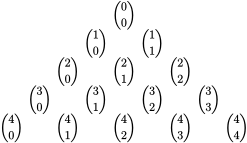
\includegraphics[width=\linewidth]{./img/pascal-nCk.svg}
\end{sbspanel}%
\end{sidebyside}%
\par
This can continue as far down as we like. The recurrence relation for \({n \choose k}\) tells us that each entry in the triangle is the sum of the two entries above it. The entries on the sides of the triangle are always 1. This is because \({n \choose 0} = 1\) for all \(n\) since there is only one way to pick 0 of \(n\) objects and \({n \choose n} = 1\) since there is one way to select all \(n\) out of \(n\) objects. Using the recurrence relation, and the fact that the sides of the triangle are 1's, we can easily replace all the entries above with the correct values of \({n \choose k}\). Doing so gives us \terminology{Pascal's triangle}. \index{Pascal's triangle}%
\par
We can use Pascal's triangle to calculate binomial coefficients. For example, using the triangle below, we can find \({12 \choose 6} = 924\).%
\begin{sidebyside}{1}{0}{0}{0}%
\begin{sbspanel}{1}%
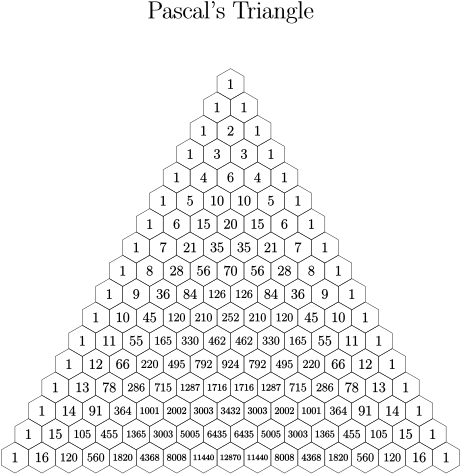
\includegraphics[width=\linewidth]{./img/pascal-large.svg}
\end{sbspanel}%
\end{sidebyside}%
\end{subsubsectionptx}
\end{subsectionptx}
%
%
\typeout{************************************************}
\typeout{Subsection 6.1.2 Today's Screencast}
\typeout{************************************************}
%
\begin{subsectionptx}{Today's Screencast}{}{Today's Screencast}{}{}{g:subsection:idm233528160016}
\begin{insight}{}{g:insight:idm233528159536}%
\setlength{\qrsize}{9em}
\setlength{\previewwidth}{\linewidth}
\addtolength{\previewwidth}{-\qrsize}
\begin{tcbraster}[raster columns=2, raster column skip=1pt, raster halign=center, raster force size=false, raster left skip=0pt, raster right skip=0pt]%
\begin{tcolorbox}[previewstyle, width=\previewwidth]%
\mono{No preview image available}%
\end{tcolorbox}%
\begin{tcolorbox}[qrstyle]%
[QR LINK]\end{tcolorbox}%
\end{tcbraster}%
\end{insight}
\end{subsectionptx}
%
%
\typeout{************************************************}
\typeout{Subsection 6.1.3 If you missed class today}
\typeout{************************************************}
%
\begin{subsectionptx}{If you missed class today}{}{If you missed class today}{}{}{g:subsection:idm233528158992}
%
\begin{enumerate}
\item{}Work through today's outline and read the marked pages in the book.%
\item{}Watch the screencast above.%
\item{}Submit any homework\slash{}assignments due today (check our \href{https://dordt.instructure.com/courses/3110050}{Canvas course} or the \href{https://prof.mkjanssen.org/ds/index.html\#schedule}{syllabus schedule} to see what's due).%
\item{}\href{mailto:mike.janssen@dordt.edu}{Send Dr. Janssen an email} or \href{https://calendly.com/mkjanssen/student-hours}{set up a student hours appointment} if you have any questions!%
\end{enumerate}
\end{subsectionptx}
\end{sectionptx}
%
%
\typeout{************************************************}
\typeout{Section 6.2 Feb. 19: Permutations and Combinations}
\typeout{************************************************}
%
\begin{sectionptx}{Feb. 19: Permutations and Combinations}{}{Feb. 19: Permutations and Combinations}{}{}{x:section:Feb-19}
%
%
\typeout{************************************************}
\typeout{Subsubsection 6.2.1 Permutations}
\typeout{************************************************}
%
\begin{subsubsectionptx}{Permutations}{}{Permutations}{}{}{g:subsubsection:idm233528153952}
\begin{investigation}{}{p:investigation:bpD}%
You have a bunch of chips which come in five different colors: red, blue, green, purple and yellow.%
\begin{enumerate}
\item{}How many different two-chip stacks can you make if the bottom chip must be red or blue? Explain your answer using both the additive and multiplicative principles.%
\item{}How many different three-chip stacks can you make if the bottom chip must be red or blue and the top chip must be green, purple or yellow? How does this problem relate to the previous one?%
\item{}How many different three-chip stacks are there in which no color is repeated? What about four-chip stacks?%
\item{}Suppose you wanted to take three different colored chips and put them in your pocket. How many different choices do you have? What if you wanted four different colored chips? How do these problems relate to the previous one?%
\end{enumerate}
%
\par\smallskip%
\noindent\textbf{\blocktitlefont Solution}.\hypertarget{g:solution:idm233528145424}{}\quad{}%
\begin{enumerate}
\item{}If the bottom chip must be red or blue, there are two choices there. Then there are five choices for the next (top) chip, so \(2\cdot 5 = 10\).%
\item{}For each of the 10 stacks from the previous part, there are three choices for the new top chip, so \(3\cdot 10 = 30\) choices in total.%
\item{}I read the problem with order mattering, e.g., RBY is a different stack than YBR. First, choose the three distinct colors from the five in \(\binom{5}{3}\) ways. For each choice of three colors, there are \(3\cdot 2\cdot 2 = 6\) ways to order them. This leaves 60 total stacks.%
\par
If we're building a stack of four chips, there are 5 choices of which chip to leave out and \(4!\) ways to order the colors once they're selected, for \(5! = 120\) orderings.%
\item{}If we only want to choose the colors, there are \(\binom{5}{3}\) and \(\binom{5}{4}\) ways to do so.%
\end{enumerate}
\end{investigation}%
\begin{definition}{}{g:definition:idm233528139568}%
A \terminology{permutation} is a (possible) rearrangement of objects.%
\end{definition}
\begin{question}{}{g:question:idm233528138672}%
How many permutations are there of the numbers \(1,2,3,4,5\)?%
\end{question}
A piece of notation is helpful here: \(n!\), read ``\(n\) factorial'', \index{factorial} is the product of all positive integers less than or equal to \(n\) (for reasons of convenience, we also define 0! to be 1). So the number of permutation of 6 letters, as seen in the previous example is \(6! = 6\cdot 5 \cdot 4 \cdot 3 \cdot 2 \cdot 1\). This generalizes:%
\begin{assemblage}{Permutations of \(n\) elements.}{x:assemblage:formula-permutations}%
There are \(n! = n\cdot (n-1)\cdot (n-2)\cdot \cdots \cdot 2\cdot 1\) permutations of \(n\) (distinct) elements.%
\end{assemblage}
\begin{exploration}{}{g:exploration:idm233528130192}%
How many functions \(f: \set{1,2,3,4,5,6} \to \set{a,b,c,d,e,f}\) are there? How many of them are bijective?%
\par\smallskip%
\noindent\textbf{\blocktitlefont Solution}.\hypertarget{g:solution:idm233528129056}{}\quad{}There are \(6^6\) total functions: six choices for each of the six elements of the domain. However, note that a bijection corresponds to a permutation of the letters a through f. There are \(6!\) such orderings and thus \(45,936\) non-bijective functions.%
\end{exploration}%
\begin{exploration}{}{g:exploration:idm233528127040}%
Consider the set \(A = \set{a,b,c,d,e,f,g,h}\).%
%
\begin{enumerate}
\item{}How many ways are there to permute all the elements of \(A\)?%
\item{}How many 7-letter ``words'' (that is, strings of letters) can you make from the elements of \(A\)? Assume no repeated letters.%
\item{}How many 6-letter words can you make from the elements of \(A\)? Assume no repeated letters.%
\item{}Suppose now that \(X\) is a set of cardinality \(n\). How many ways are there to order \(k\le n\) distinct objects from \(X\)? Conjecture a formula.%
\item{}Suppose \(f: S\to T\) is a function with \(\card{S} = k\) and \(\card{T} = n\). How many such functions \(f\) are injective?%
\end{enumerate}
\par\smallskip%
\noindent\textbf{\blocktitlefont Solution}.\hypertarget{g:solution:idm233528119136}{}\quad{}%
\begin{enumerate}
\item{}There are \(7!\) such permutations.%
\item{}It depends: if letters cannot be repeated, then this is the same as the previous question. If letters \emph{can} be repeated, it's a much more complicated question.%
\item{}First, we choose the six letters we'll use: there are \(\binom{7}{6}\) ways to do that. Then there are \(6!\) ways to arrange them, for a total of \(7!\) six-letter words.%
\item{}First, we choose the \(\binom{n}{k}\) objects. Then we order them \(k!\) ways, for a total of \(\binom{n}{k}\cdot k!\) possible orderings of \(k\) objects chosen from \(n\) distinct objects.%
\item{}This is the same question as the previous one!%
\end{enumerate}
\end{exploration}%
\begin{assemblage}{\(k\)-permutations of \(n\) elements.}{p:assemblage:Krs}%
\(P(n,k)\) is the number of \terminology{\(k\)-permutations of \(n\) elements}, the number of ways to \emph{arrange} \(k\) objects chosen from \(n\) distinct objects.%
\begin{equation*}
P(n,k) = \frac{n!}{(n-k)!} = n(n-1)(n-2)\cdots (n-(k-1))\text{.}
\end{equation*}
%
\end{assemblage}
Here is another way to find the number of \(k\)-permutations of \(n\) elements: first select which \(k\) elements will be in the permutation, then count how many ways there are to arrange them. Once you have selected the \(k\) objects, we know there are \(k!\) ways to arrange (permute) them. But how do you select \(k\) objects from the \(n\)? You have \(n\) objects, and you need to \emph{choose} \(k\) of them. You can do that in \({n \choose k}\) ways. Then for each choice of those \(k\) elements, we can permute \emph{them} in \(k!\) ways. Using the multiplicative principle, we get another formula for \(P(n,k)\):%
\begin{equation*}
P(n,k) = {n \choose k}\cdot k!\text{.}
\end{equation*}
%
\par
Now since we have a closed formula for \(P(n,k)\) already, we can substitute that in:%
\begin{equation*}
\frac{n!}{(n-k)!} = {n \choose k} \cdot k!\text{.}
\end{equation*}
%
\par
If we divide both sides by \(k!\) we get a closed formula for \({n \choose k}\).%
\begin{assemblage}{Closed formula for \({n \choose k}\).}{p:assemblage:qyB}%
%
\begin{equation*}
{n \choose k} = \frac{n!}{(n-k)!k!} = \frac{n(n-1)(n-2)\cdots(n-(k-1))}{k(k-1)(k-2)\cdots 1}\text{.}
\end{equation*}
%
\end{assemblage}
\index{combination!vs permutation}\index{permutation!vs combination} We say \(P(n,k)\) counts \emph{permutations}, and \({n \choose k}\) counts \emph{combinations}. The formulas for each are very similar, there is just an extra \(k!\) in the denominator of \({n \choose k}\). That extra \(k!\) accounts for the fact that \({n \choose k}\) does not distinguish between the different orders that the \(k\) objects can appear in. We are just selecting (or choosing) the \(k\) objects, not arranging them. Perhaps ``combination'' is a misleading label. We don't mean it like a combination lock (where the order would definitely matter). Perhaps a better metaphor is a combination of flavors \textemdash{} you just need to decide which flavors to combine, not the order in which to combine them.%
\end{subsubsectionptx}
%
%
\typeout{************************************************}
\typeout{Subsection 6.2.1 Today's Screencast}
\typeout{************************************************}
%
\begin{subsectionptx}{Today's Screencast}{}{Today's Screencast}{}{}{g:subsection:idm233528153824}
\begin{insight}{}{g:insight:idm233528082432}%
\setlength{\qrsize}{9em}
\setlength{\previewwidth}{\linewidth}
\addtolength{\previewwidth}{-\qrsize}
\begin{tcbraster}[raster columns=2, raster column skip=1pt, raster halign=center, raster force size=false, raster left skip=0pt, raster right skip=0pt]%
\begin{tcolorbox}[previewstyle, width=\previewwidth]%
\mono{No preview image available}%
\end{tcolorbox}%
\begin{tcolorbox}[qrstyle]%
[QR LINK]\end{tcolorbox}%
\end{tcbraster}%
\end{insight}
\end{subsectionptx}
\end{sectionptx}
\end{chapterptx}
%
%
\typeout{************************************************}
\typeout{Chapter 7 Week 7: Feb. 22-26}
\typeout{************************************************}
%
\begin{chapterptx}{Week 7: Feb. 22-26}{}{Week 7: Feb. 22-26}{}{}{x:chapter:Week-07}
\begin{introduction}{}%
This week we head further up and further in to counting problems. We glimpse the art of combinatorial proof, and take a look at a counting technique known as ``stars and bars''. Also, on Wednesday, we'll discuss Chs. 6-7 of M4HF.%
\end{introduction}%
%
%
\typeout{************************************************}
\typeout{Section 7.1 Feb. 22: Combinatorial Proofs I}
\typeout{************************************************}
%
\begin{sectionptx}{Feb. 22: Combinatorial Proofs I}{}{Feb. 22: Combinatorial Proofs I}{}{}{x:section:Feb-22}
\begin{introduction}{}%
\begin{assemblage}{Motivating Questions.}{g:assemblage:idm233528079520}%
Here are some questions we'll consider. %
\begin{enumerate}
\item{}What is a combinatorial proof?%
\item{}How can we improve at writing combinatorial proofs?%
\end{enumerate}
%
\end{assemblage}
\end{introduction}%
%
%
\typeout{************************************************}
\typeout{Subsection 7.1.1 Outline}
\typeout{************************************************}
%
\begin{subsectionptx}{Outline}{}{Outline}{}{}{g:subsection:idm233528077312}
Today's material comes from \href{http://discrete.openmathbooks.org/dmoi3/sec_comb-proofs.html}{Section 1.4} of the book. You're encouraged to read it before coming to class.%
%
%
\typeout{************************************************}
\typeout{Subsubsection 7.1.1.1 From Last Time}
\typeout{************************************************}
%
\begin{subsubsectionptx}{From Last Time}{}{From Last Time}{}{}{g:subsubsection:idm233528075984}
\begin{exploration}{}{g:exploration:idm233528075424}%
Prof. Clark is once again getting ready to order pizzas for the next Pizza and Presentation. Recall from \hyperref[x:investigation:invest-pizzas]{Investigation~{\xreffont\ref{x:investigation:invest-pizzas}}} that there are:%
%
\begin{itemize}[label=\textbullet]
\item{}Three choices for crusts (thin, hand-tossed, thick)%
\item{}Three choices for sauce (red, white, BBQ)%
\item{}Fifteen choices for toppings%
\end{itemize}
How many different pizzas are possible if Prof. Clark can make one choice for crust, one choice for sauce, and then choose any number of toppings?%
\par\smallskip%
\noindent\textbf{\blocktitlefont Solution}.\hypertarget{g:solution:idm233528072528}{}\quad{}The main problem is to figure out the number of choices for toppings. We will assume no repeated toppings (or at least that, e.g., double pepperoni is the same as single pepperoni for the purposes of counting combinations of toppings). We also assume that the order in which toppings are added does not matter (possibly contentious!). Note that for \(0 \le k \le 15\), there are \(\binom{15}{k}\) ways to make a \(k\)-topping pizza. Then there are%
\begin{equation*}
3\cdot 3\cdot \sum\limits_{k=0}^{15} \binom{15}{k} = 294,912
\end{equation*}
possible pizzas.%
\end{exploration}%
\end{subsubsectionptx}
%
%
\typeout{************************************************}
\typeout{Subsubsection 7.1.1.2 A motivating investigation}
\typeout{************************************************}
%
\begin{subsubsectionptx}{A motivating investigation}{}{A motivating investigation}{}{}{g:subsubsection:idm233528069728}
\begin{investigation}{}{p:investigation:UJt}%
%
\begin{enumerate}
\item{}The Stanley Cup is decided in a best of 7 tournament between two teams. In how many ways can your team win? Let's answer this question two ways:%
\begin{enumerate}
\item{}How many of the 7 games does your team need to win? How many ways can this happen?%
\item{}What if the tournament goes all 7 games? So you win the last game. How many ways can the first 6 games go down?%
\item{}What if the tournament goes just 6 games? How many ways can this happen? What about 5 games? 4 games?%
\item{}What are the two different ways to compute the number of ways your team can win? Write down an equation involving binomial coefficients (that is, \({n \choose k}\)'s). What pattern in \hyperref[x:image:pascal-large]{Pascal's triangle} is this an example of?%
\end{enumerate}
%
\item{}Generalize. What if the rules changed and you played a best of \(9\) tournament (5 wins required)? What if you played an \(n\) game tournament with \(k\) wins required to be named champion?%
\end{enumerate}
%
\par\smallskip%
\noindent\textbf{\blocktitlefont Solution}.\hypertarget{g:solution:idm233528055760}{}\quad{}%
\begin{enumerate}
\item{}%
\begin{enumerate}
\item{}This is the same as counting the number of weight 4 bit strings of length 7, which is \(\binom{7}{4} = 35\).%
\item{}This is the same as counting the number of weight 3 bitstrings of length 6, which is \(\binom{6}{3} = 20 ways\).%
\item{}This is the number of weight 4 bitstrings of length 6, which is \(\binom{6}{4} = 15\). The same for 5 games (5 ways) and 4 games (1 way).%
\item{}One way is \(\binom{7}{4}\). Another is \(\binom{6}{3} + \binom{6}{4}\).%
\end{enumerate}
%
\item{}In general, as we've seen, \(\binom{n}{k} = \binom{n-1}{k-1}+\binom{n-1}{k}\).%
\end{enumerate}
\end{investigation}%
This is an example of a \terminology{combinatorial proof}, which seeks to establish an identity (that is, an equation) by asking a counting question, and answering it in two different ways. Since the two methods answer the same question, they must in fact be equal. We now explore some additional examples.%
\end{subsubsectionptx}
%
%
\typeout{************************************************}
\typeout{Subsubsection 7.1.1.3 Pascal's Triangle, revisited}
\typeout{************************************************}
%
\begin{subsubsectionptx}{Pascal's Triangle, revisited}{}{Pascal's Triangle, revisited}{}{}{g:subsubsection:idm233528049904}
\begin{exploration}{}{g:exploration:idm233528049520}%
Recall Pascal's triangle:%
\begin{image}{0}{1}{0}%
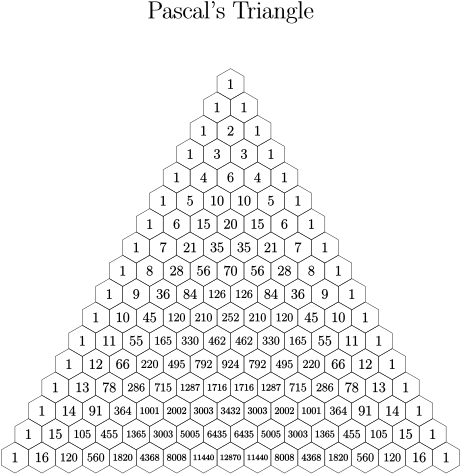
\includegraphics[width=\linewidth]{./img/pascal-large.svg}
\end{image}%
There are lots of patterns hidden away in the triangle, enough to fill a reasonably sized book. Here are just a few of the most obvious ones:%
\begin{enumerate}
\item{}The entries on the border of the triangle are all 1.%
\item{}Any entry not on the border is the sum of the two entries above it.%
\item{}The triangle is symmetric. In any row, entries on the left side are mirrored on the right side.%
\item{}The sum of all entries on a given row is a power of 2. (You should check this!)%
\end{enumerate}
We can state these identities in terms of binomial coefficients as follows.%
%
\begin{enumerate}
\item{}\({n \choose 0} = 1\) and \({n \choose n} = 1\).%
\item{}\({n \choose k} = {n-1 \choose k-1} + {n-1 \choose k}\).%
\item{}\({n \choose k} = {n \choose n-k}\).%
\item{}\({n\choose 0} + {n \choose 1} + {n \choose 2} + \cdots + {n \choose n} = 2^n\).%
\end{enumerate}
Try to establish at least one by answering a question in two different ways.%
\end{exploration}%
\end{subsubsectionptx}
%
%
\typeout{************************************************}
\typeout{Subsubsection 7.1.1.4 More Examples}
\typeout{************************************************}
%
\begin{subsubsectionptx}{More Examples}{}{More Examples}{}{}{g:subsubsection:idm233528036592}
Note that in many cases, we \emph{can} use algebra to establish these identities.%
\begin{example}{}{p:example:LpH}%
Give an algebraic proof for the binomial identity%
\begin{equation*}
{n \choose k} = {n-1\choose k-1} + {n-1 \choose k}\text{.}
\end{equation*}
%
\par\smallskip%
\noindent\textbf{\blocktitlefont Solution}.\hypertarget{p:solution:AQC}{}\quad{}\begin{solutionproof}
By the definition of \({n \choose k}\), we have%
\begin{equation*}
{n-1 \choose k-1} = \frac{(n-1)!}{(n-1-(k-1))!(k-1)!} = \frac{(n-1)!}{(n-k)!(k-1)!}
\end{equation*}
and%
\begin{equation*}
{n-1 \choose k} = \frac{(n-1)!}{(n-1-k)!k!}\text{.}
\end{equation*}
%
\par
Thus, starting with the right-hand side of the equation:%
\begin{align*}
{n-1 \choose k-1} + {n-1 \choose k} \amp = \frac{(n-1)!}{(n-k)!(k-1)!}+ \frac{(n-1)!}{(n-1-k)!\,k!}\\
\amp = \frac{(n-1)!k}{(n-k)!\,k!} + \frac{(n-1)!(n-k)}{(n-k)!\,k!}\\
\amp = \frac{(n-1)!(k+n-k)}{(n-k)!\,k!}\\
\amp = \frac{n!}{(n-k)!\, k!}\\
\amp = {n \choose k}\text{.}
\end{align*}
%
\par
The second line (where the common denominator is found) works because \(k(k-1)! = k!\) and \((n-k)(n-k-1)! = (n-k)!\).%
\end{solutionproof}
\end{example}
\begin{theorem}{}{}{g:theorem:idm233528025904}%
%
\begin{equation*}
1\cdot 8 + 2\cdot 7 + 3\cdot 6 + \cdots + 8\cdot 1 = \binom{10}{3}.
\end{equation*}
\end{theorem}
\begin{proof}{}{g:proof:idm233528025280}
The question we ask is: how many 3-element subsets of \(A= \set{1,2,\ldots, 10}\) are there? One answer (based on previous work) is \(\binom{10}{3}\).%
\par
For the other answer, consider a three element subset \(\set{a,b,c}\) with \(a \lt b \lt c\). We count based on values for \(b\).%
%
\begin{itemize}[label=\textbullet]
\item{}If \(b=2\), then there is one choice for \(a\) and 8 choices for \(c\), so \(1\cdot 8\) choices in total.%
\item{}If \(b=3\), there there are 2 choicesa for \(a\) and \(7\) choices for \(c\), so \(2\cdot 7\) choices in total.%
\item{}Etc. etc.%
\end{itemize}
The identity is established.%
\end{proof}
\begin{theorem}{}{}{g:theorem:idm233528017280}%
%
\begin{equation*}
\binom{n}{k} \binom{n-k}{r} = \binom{n}{r} \binom{n-r}{k}
\end{equation*}
\end{theorem}
\begin{proof}{}{g:proof:idm233528016656}
Suppose Prof. Clark, fresh off the success of Pizza and a Presentation, is looking to establish two committees of people interested in helping organize future versions: a pizza-planning committee for choosing the pizzas and consisting of \(k\) members; and a speaker-planning committee for choosing speakers and consisting of \(r\) members. A total of \(n\) people have expressed interest in serving on one of the committees, and Prof. Clark decides that no one should be on both committees. How many ways are there for him to assign members to the committees?%
\par
On the one hand, there are \(\binom{n}{k}\) ways to construct the pizza-planning committee. Then, there are \(n-k\) volunteers remaining, so there are \(\binom{n-k}{r}\) ways to construct the speaker-planning committee and so \(\binom{n}{k} \binom{n-k}{r}\) ways of constructing both committees.%
\par
On the other hand, perhaps we construct the speaker-planning committee first; there are \(\binom{n}{r}\) ways to do so. Then we choose the \(k\)-member pizza-planning committee from the remaining \(n-r\) interested volunteers.%
\end{proof}
\end{subsubsectionptx}
\end{subsectionptx}
%
%
\typeout{************************************************}
\typeout{Subsection 7.1.2 Today's Screencast}
\typeout{************************************************}
%
\begin{subsectionptx}{Today's Screencast}{}{Today's Screencast}{}{}{g:subsection:idm233528010480}
\begin{insight}{}{g:insight:idm233528010096}%
\setlength{\qrsize}{9em}
\setlength{\previewwidth}{\linewidth}
\addtolength{\previewwidth}{-\qrsize}
\begin{tcbraster}[raster columns=2, raster column skip=1pt, raster halign=center, raster force size=false, raster left skip=0pt, raster right skip=0pt]%
\begin{tcolorbox}[previewstyle, width=\previewwidth]%
\mono{No preview image available}%
\end{tcolorbox}%
\begin{tcolorbox}[qrstyle]%
[QR LINK]\end{tcolorbox}%
\end{tcbraster}%
\end{insight}
\end{subsectionptx}
%
%
\typeout{************************************************}
\typeout{Subsection 7.1.3 If you missed class today}
\typeout{************************************************}
%
\begin{subsectionptx}{If you missed class today}{}{If you missed class today}{}{}{g:subsection:idm233528009712}
%
\begin{enumerate}
\item{}Work through today's outline and read the marked pages in the book.%
\item{}Watch the screencast above.%
\item{}Submit any homework\slash{}assignments due today (check our \href{https://dordt.instructure.com/courses/3110050}{Canvas course} or the \href{https://prof.mkjanssen.org/ds/index.html\#schedule}{syllabus schedule} to see what's due).%
\item{}\href{mailto:mike.janssen@dordt.edu}{Send Dr. Janssen an email} or \href{https://calendly.com/mkjanssen/student-hours}{set up a student hours appointment} if you have any questions!%
\end{enumerate}
\end{subsectionptx}
\end{sectionptx}
%
%
\typeout{************************************************}
\typeout{Section 7.2 Feb. 24: Reading Discussion and Combinatorial Proofs II}
\typeout{************************************************}
%
\begin{sectionptx}{Feb. 24: Reading Discussion and Combinatorial Proofs II}{}{Feb. 24: Reading Discussion and Combinatorial Proofs II}{}{}{x:section:Feb-24}
\begin{introduction}{}%
\begin{assemblage}{Motivating Questions.}{g:assemblage:idm233528004528}%
Here are some questions we'll consider. %
\begin{enumerate}
\item{}How can struggle be productive?%
\item{}What role does mathematics play in helping us discern truth?%
\item{}How can we establish identities by counting in two different ways?%
\end{enumerate}
%
\end{assemblage}
\end{introduction}%
%
%
\typeout{************************************************}
\typeout{Subsection 7.2.1 Outline}
\typeout{************************************************}
%
\begin{subsectionptx}{Outline}{}{Outline}{}{}{g:subsection:idm233528002176}
%
%
\typeout{************************************************}
\typeout{Subsubsection 7.2.1.1 Reading Discussion}
\typeout{************************************************}
%
\begin{subsubsectionptx}{Reading Discussion}{}{Reading Discussion}{}{}{g:subsubsection:idm233528001792}
\begin{principle}{}{}{g:principle:idm233528001408}%
Discuss the reading with those sitting nearby. You may consider the following questions as a starting place, but feel free to follow the discussion wherever it leads.%
%
\begin{itemize}[label=\textbullet]
\item{}What mathematical laws, truths, or ideas do you rely on in your everyday life?%
\item{}Many things in the universe change over time. Do you find it surprising that the laws and theorems of mathematics do not change? Are there similar unchanging truths in other areas of inquiry?%
\item{}What does knowing the ``whole truth'' of an idea\slash{}topic look like? To what degree is knowing the whole truth possible?%
\item{}How can mathematical thinking equip you to converse with and respect people who hold different views than you on a subject?%
\item{}In what areas of your life is your mindset fixed? In what areas do you have a growth mindset?%
\item{}Describe a time in which you have struggled productively. How can you recognize when struggle turns unproductive?%
\end{itemize}
\end{principle}
\end{subsubsectionptx}
%
%
\typeout{************************************************}
\typeout{Subsubsection 7.2.1.2 More Combinatorial Proofs}
\typeout{************************************************}
%
\begin{subsubsectionptx}{More Combinatorial Proofs}{}{More Combinatorial Proofs}{}{}{g:subsubsection:idm233527997568}
\begin{exploration}{}{g:exploration:idm233527997184}%
Use a combinatorial proof to establish the following identities. Bonus points for humor and creativity.%
%
\begin{enumerate}
\item{}%
\begin{equation*}
\binom{w}{p} \binom{p}{m} = \binom{w}{m} \binom{w-m}{p-m}
\end{equation*}
%
\item{}%
\begin{equation*}
\sum\limits_{k=0}^n \left(\binom{n}{k}\right)^2 = \binom{2n}{n}
\end{equation*}
%
\item{}%
\begin{equation*}
\binom{n+m}{r} = \sum\limits_{i=0}^r \binom{n}{i} \binom{m}{r-i}
\end{equation*}
%
\end{enumerate}
\par\smallskip%
\noindent\textbf{\blocktitlefont Solution}.\hypertarget{g:solution:idm233527993904}{}\quad{}%
\begin{enumerate}
\item{}Consider a \(w\) volunteers for a committee with \(p\) members containing a subcommittee of \(m\) members. We can choose the \(p\) committee members and then the \(m\) subcommittee members, or choose the \(m\) subcommittee members and then the remaining \(p-m\) committee members.%
\item{}How many ways are there to make an \(n\)-person committee chosen \(n\) Dordt students and \(n\) Northwestern students? On the one hand, \(\binom{2n}{n}\). On the other hand, recall that \(\binom{n}{k} = \binom{n}{n-k}\), so the sum can be rewritten as%
\begin{equation*}
\sum\limits_{k=0}^n \left(\binom{n}{k}\right)^2 = \sum\limits_{k=0}^n \binom{n}{k} \binom{n}{n-k}.
\end{equation*}
Let \(k\) be the number of Dordt students. Then for each \(k\) we choose \(k\) Dordt students in \(\binom{n}{k}\) ways and \(n-k\) NWC students in \(\binom{n}{n-k}\) ways.%
\item{}This is the same story as the previous one, only now there are \(n\) Dordt students and \(m\) NWC students with a desired committee size of \(r\) students.%
\end{enumerate}
\end{exploration}%
\begin{exploration}{}{g:exploration:idm233527983024}%
Find combinatorial proofs for the following identities. Bonus points for humor and creativity.%
%
\begin{enumerate}
\item{}%
\begin{equation*}
n\binom{n-1}{k} = (k+1) \binom{n}{k+1}
\end{equation*}
%
\item{}%
\begin{equation*}
n\binom{n-1}{k-1} = k\binom{n}{k}
\end{equation*}
%
\item{}%
\begin{equation*}
n(n-1)\binom{n-2}{k-2} = k(k-1)\binom{n}{k}
\end{equation*}
%
\end{enumerate}
\par\smallskip%
\noindent\textbf{\blocktitlefont Solution}.\hypertarget{g:solution:idm233527979744}{}\quad{}%
\begin{enumerate}
\item{}How can we choose a committee of \(k+1\) members from \(n\) people and designate a chair? First choose the chair (\(n\) ways), then the remaining \(k\) members. Or, choose the committee (\(\binom{n}{k+1}\) ways), then the chair from among the committee members.%
\item{}Basically the same question as the previous one, only now our committee has \(k\) members.%
\item{}Similar question as before, only now we have a chair and vice-chair.%
\end{enumerate}
\end{exploration}%
\begin{assemblage}{Challenge.}{g:assemblage:idm233527975984}%
Calculate \(\sum_{k=0}^n \binom{n}{2k}\) for \(n=2,3,4\). Use these data to find an identity of the form%
\begin{equation*}
\sum\limits_{k=0}^n \binom{n}{2k} = ???
\end{equation*}
Now prove your identity holds.%
\end{assemblage}
\end{subsubsectionptx}
\end{subsectionptx}
%
%
\typeout{************************************************}
\typeout{Subsection 7.2.2 Today's Screencast}
\typeout{************************************************}
%
\begin{subsectionptx}{Today's Screencast}{}{Today's Screencast}{}{}{g:subsection:idm233527973552}
\begin{insight}{}{g:insight:idm233527973168}%
\setlength{\qrsize}{9em}
\setlength{\previewwidth}{\linewidth}
\addtolength{\previewwidth}{-\qrsize}
\begin{tcbraster}[raster columns=2, raster column skip=1pt, raster halign=center, raster force size=false, raster left skip=0pt, raster right skip=0pt]%
\begin{tcolorbox}[previewstyle, width=\previewwidth]%
\mono{No preview image available}%
\end{tcolorbox}%
\begin{tcolorbox}[qrstyle]%
[QR LINK]\end{tcolorbox}%
\end{tcbraster}%
\end{insight}
\end{subsectionptx}
%
%
\typeout{************************************************}
\typeout{Subsection 7.2.3 If you missed class today}
\typeout{************************************************}
%
\begin{subsectionptx}{If you missed class today}{}{If you missed class today}{}{}{g:subsection:idm233527972704}
%
\begin{enumerate}
\item{}Work through today's outline and read the marked pages in the book.%
\item{}Watch the screencast above.%
\item{}Submit any homework\slash{}assignments due today (check our \href{https://dordt.instructure.com/courses/3110050}{Canvas course} or the \href{https://prof.mkjanssen.org/ds/index.html\#schedule}{syllabus schedule} to see what's due).%
\item{}\href{mailto:mike.janssen@dordt.edu}{Send Dr. Janssen an email} or \href{https://calendly.com/mkjanssen/student-hours}{set up a student hours appointment} if you have any questions!%
\end{enumerate}
\end{subsectionptx}
\end{sectionptx}
%
%
\typeout{************************************************}
\typeout{Section 7.3 Feb. 26: Stars and Bars}
\typeout{************************************************}
%
\begin{sectionptx}{Feb. 26: Stars and Bars}{}{Feb. 26: Stars and Bars}{}{}{x:section:Feb-26}
\begin{introduction}{}%
\begin{assemblage}{Motivating Questions.}{g:assemblage:idm233527967568}%
Here are some questions we'll consider. %
\begin{enumerate}
\item{}How can we count the ways to distribute identical objects among people?%
\item{}What other types of problems does the stars and bars method allow us to solve?%
\end{enumerate}
%
\end{assemblage}
\end{introduction}%
%
%
\typeout{************************************************}
\typeout{Subsection 7.3.1 Outline}
\typeout{************************************************}
%
\begin{subsectionptx}{Outline}{}{Outline}{}{}{g:subsection:idm233527965264}
Today's material comes from \href{http://discrete.openmathbooks.org/dmoi3/sec_stars-and-bars.html}{Section 1.5} of the book. You're encouraged to read it before coming to class.%
%
%
\typeout{************************************************}
\typeout{Subsubsection 7.3.1.1 Intro to Stars and Bars}
\typeout{************************************************}
%
\begin{subsubsectionptx}{Intro to Stars and Bars}{}{Intro to Stars and Bars}{}{}{g:subsubsection:idm233527964016}
\begin{investigation}{}{p:investigation:bbv}%
Suppose you have some number of identical Rubik's cubes to distribute to your friends. Imagine you start with a single row of the cubes.%
\begin{enumerate}
\item{}Find the number of different ways you can distribute the cubes provided:%
\par
%
\begin{enumerate}
\item{}You have 3 cubes to give to 2 people.%
\item{}You have 4 cubes to give to 2 people.%
\item{}You have 5 cubes to give to 2 people.%
\item{}You have 3 cubes to give to 3 people.%
\item{}You have 4 cubes to give to 3 people.%
\item{}You have 5 cubes to give to 3 people.%
\end{enumerate}
%
\item{}Make a conjecture about how many different ways you could distribute 7 cubes to 4 people. Explain.%
\item{}What if each person were required to get \emph{at least one} cube? How would your answers change?%
\end{enumerate}
%
\par\smallskip%
\noindent\hypertarget{g:solution:idm233527948016}{}In general, if we want to distribute \(n\) cubes to \(k\) people, we can lay the cubes out and place \(k-1\) dividers (bars). We can think of this as a bit string if we want: there are then \(\binom{n+k-1}{k-1}\) ways to distribute them.%
\par
If everyone is required to get at least one cube, distribute those cubes first; then there are \(n-k\) cubes to distribute among \(k\) people, so \(\binom{n-k+k-1}{k-1} = \binom{n-1}{k-1}\) ways to do it.%
\end{investigation}%
\end{subsubsectionptx}
%
%
\typeout{************************************************}
\typeout{Subsubsection 7.3.1.2 Stars and Bars Charts}
\typeout{************************************************}
%
\begin{subsubsectionptx}{Stars and Bars Charts}{}{Stars and Bars Charts}{}{}{g:subsubsection:idm233527944208}
Consider the following counting problem:%
\begin{quote}%
You have 7 cookies to give to 4 kids. How many ways can you do this?%
\end{quote}
Take a moment to think about how you might solve this problem. You may assume that it is acceptable to give a kid no cookies. Also, the cookies are all identical and the order in which you give out the cookies does not matter.%
\par
All we really need to do is say when to switch from one kid to the next. In terms of cookies, we need to say after how many cookies do we stop giving cookies to the first kid and start giving cookies to the second kid. And then after how many do we switch to the third kid? And after how many do we switch to the fourth? So the way we'll represent an outcome is like this:%
\begin{equation*}
***|*|*|**\text{.}
\end{equation*}
%
\par
Three cookies go to the first kid, then we switch and give one cookie to the second kid, then switch, one to the third kid, switch, two to the fourth kid. Notice that we need 7 stars and 3 bars \textendash{} one star for each cookie, and one bar for each switch between kids, so one fewer bars than there are kids (we don't need to switch after the last kid \textendash{} we are done).%
\par
Why have we done all of this? Simple: to count the number of ways to distribute 7 cookies to 4 kids, all we need to do is count how many \emph{stars and bars} charts there are. But a \terminology{stars and bars chart} \index{stars and bars!chart} is just a string of symbols, some stars and some bars. If instead of stars and bars we would use 0's and 1's, it would just be a bit string. \index{bit string!relation to stars and bars} We know how to count those. First, let's make sure we really know what we're doing.%
\begin{exploration}{}{g:exploration:idm233527934416}%
What is the cookie\slash{}kid distribution, if any, described by the following stars and bars charts?%
%
\begin{enumerate}
\item{}\(\displaystyle *|**|**|**\)%
\item{}\(\displaystyle |***||****\)%
\item{}\(\displaystyle |||*******\)%
\end{enumerate}
How many ways are there to distribute 7 cookies to 4 kids?%
\end{exploration}%
\begin{exploration}{Owls and Cats (DMWD).}{g:exploration:idm233527931536}%
Suppose we have six teal owls and three orange cats. How many ways are there to arrange them in a line so no two cats sit next to each other?%
\par\smallskip%
\noindent\textbf{\blocktitlefont Solution}.\hypertarget{g:solution:idm233527930576}{}\quad{}What does it mean for no two cats to sit next to each other? It means we must place an owl between the first pair of cats and an owl between the second pair. This leaves four owls to distribute between the 3 cats, or \(\binom{4+2}{2} = 15\) ways.\end{exploration}%
\begin{exploration}{}{g:exploration:idm233527929664}%
An ogre distributes 43 cupcakes to 12 baby mice. How many ways can this be done?%
\par\smallskip%
\noindent\textbf{\blocktitlefont Solution}.\hypertarget{g:solution:idm233527928992}{}\quad{}The stars are the cupcakes and 11 dividers are needed. So there are \(\binom{43+11}{11} = 95,722,852,680\) ways to do it.\end{exploration}%
\begin{exploration}{}{g:exploration:idm233527928224}%
How many integer solutions are there to the equation%
%
\begin{equation*}
x_1 + x_2 + x_3  x_4 + x_5 = 15
\end{equation*}
if %
\begin{enumerate}
\item{}\(x_i \ge 0\) for each \(i\)?%
\item{}\(x_i \gt 0\) for each \(i\)?%
\item{}\(x_i \ge 2\) for each \(i\)?%
\end{enumerate}
\par\smallskip%
\noindent\textbf{\blocktitlefont Solution}.\hypertarget{g:solution:idm233527923840}{}\quad{}This is the same as before. There are 15 units to assign to five boxes. So, \(\binom{15+5-1}{5-1} = 3876\).%
\par
The second one requires each variable to be at least 1, so instead we assign 10 units to 5 boxes: \(\binom{10+5-1}{5-1} = 1001\).%
\par
Last, we assign 2 units to each variable, leaving 5 to be assigned: \(\binom{5+5-1}{5-1} = 126\).%
\par
Of course, if each variable needs to be at least 3, there are \(\binom{5-1}{5-1} = 1\) ways to accomplish this.%
\end{exploration}%
\begin{exploration}{}{g:exploration:idm233527920560}%
How many ways are there to place \(k\) unlabeled balls into \(n\) labeled boxes?%
\end{exploration}%
\end{subsubsectionptx}
\end{subsectionptx}
%
%
\typeout{************************************************}
\typeout{Subsection 7.3.2 Today's Screencast}
\typeout{************************************************}
%
\begin{subsectionptx}{Today's Screencast}{}{Today's Screencast}{}{}{g:subsection:idm233527944080}
\begin{insight}{}{g:insight:idm233527919040}%
\setlength{\qrsize}{9em}
\setlength{\previewwidth}{\linewidth}
\addtolength{\previewwidth}{-\qrsize}
\begin{tcbraster}[raster columns=2, raster column skip=1pt, raster halign=center, raster force size=false, raster left skip=0pt, raster right skip=0pt]%
\begin{tcolorbox}[previewstyle, width=\previewwidth]%
\mono{No preview image available}%
\end{tcolorbox}%
\begin{tcolorbox}[qrstyle]%
[QR LINK]\end{tcolorbox}%
\end{tcbraster}%
\end{insight}
\end{subsectionptx}
%
%
\typeout{************************************************}
\typeout{Subsection 7.3.3 If you missed class today}
\typeout{************************************************}
%
\begin{subsectionptx}{If you missed class today}{}{If you missed class today}{}{}{g:subsection:idm233527918400}
%
\begin{enumerate}
\item{}Work through today's outline and read the marked pages in the book.%
\item{}Watch the screencast above.%
\item{}Submit any homework\slash{}assignments due today (check our \href{https://dordt.instructure.com/courses/3110050}{Canvas course} or the \href{https://prof.mkjanssen.org/ds/index.html\#schedule}{syllabus schedule} to see what's due).%
\item{}\href{mailto:mike.janssen@dordt.edu}{Send Dr. Janssen an email} or \href{https://calendly.com/mkjanssen/student-hours}{set up a student hours appointment} if you have any questions!%
\end{enumerate}
\end{subsectionptx}
\end{sectionptx}
\end{chapterptx}
%
%
\typeout{************************************************}
\typeout{Chapter 8 Week 8: Mar. 1-5}
\typeout{************************************************}
%
\begin{chapterptx}{Week 8: Mar. 1-5}{}{Week 8: Mar. 1-5}{}{}{x:chapter:Week-08}
\begin{introduction}{}%
This week, we look at some advanced counting techniques. We've also built in some catchup\slash{}review time, which will be useful for preparing for Exam 1 on Friday, March 5. This will be a 50-point exam covering Chapters 0 and 1. Expect a couple of short definitions followed by some straightforward questions covering sets, functions, and counting. You may find the resources in \hyperref[x:appendix:appendix-counting]{Appendix~{\xreffont\ref{x:appendix:appendix-counting}}} helpful.%
\end{introduction}%
%
%
\typeout{************************************************}
\typeout{Section 8.1 Mar. 1: Advanced PIE}
\typeout{************************************************}
%
\begin{sectionptx}{Mar. 1: Advanced PIE}{}{Mar. 1: Advanced PIE}{}{}{x:section:Mar-01}
\begin{introduction}{}%
\begin{assemblage}{Motivating Questions.}{g:assemblage:idm233527911248}%
Here are some questions we'll consider. %
\begin{enumerate}
\item{}How can we use PIE in more complicated counting questions?%
\item{}How can we translate existing counting questions to questions about counting functions?%
\end{enumerate}
%
\end{assemblage}
\end{introduction}%
%
%
\typeout{************************************************}
\typeout{Subsection 8.1.1 Outline}
\typeout{************************************************}
%
\begin{subsectionptx}{Outline}{}{Outline}{}{}{g:subsection:idm233527910656}
Today's material comes from \href{http://discrete.openmathbooks.org/dmoi3/sec_advPIE.html}{Section 1.6} of the book. You're encouraged to read it before coming to class.%
%
%
\typeout{************************************************}
\typeout{Subsubsection 8.1.1.1 Advanced PIE}
\typeout{************************************************}
%
\begin{subsubsectionptx}{Advanced PIE}{}{Advanced PIE}{}{}{g:subsubsection:idm233527907792}
\begin{investigation}{}{p:investigation:icR}%
You have 11 identical mini key-lime pies to give to 4 children. However, you don't want any kid to get more than 3 pies. How many ways can you distribute the pies?%
\begin{enumerate}
\item{}How many ways are there to distribute the pies without any restriction?%
\item{}Let's get rid of the ways that one or more kid gets too many pies. How many ways are there to distribute the pies if Al gets too many pies? What if Bruce gets too many? Or Cat? Or Dent?%
\item{}What if two kids get too many pies? How many ways can this happen? Does it matter which two kids you pick to overfeed?%
\item{}Is it possible that three kids get too many pies? If so, how many ways can this happen?%
\item{}How should you combine all the numbers you found above to answer the original question?%
\end{enumerate}
%
\par
Suppose now you have 13 pies and 7 children. No child can have more than 2 pies. How many ways can you distribute the pies?%
\par\smallskip%
\noindent\hypertarget{g:solution:idm233527898192}{}%
\begin{enumerate}
\item{}This is a stars and bars problem; there are \(\binom{11+3}{3} = 364\) ways to distribute the pies.%
\item{}Suppose Al gets 4 pies. Now he is guaranteed too many. There are 7 pies left to distribute among the four children; there are \(\binom{7 + 3}{3} = 120\) ways for Al to get too many pies. Since there are 4 children, there are \(\binom{4}{1} \cdot \binom{10}{3}\) ways for at least one child to get too many pies.%
\item{}Now suppose we give two children too many pies. There are \(\binom{4}{2}\) ways to choose the children. We'll give each four pies, leaving 3 to be distributed in \(\binom{3+3}{3}\) ways. There are then \(\binom{4}{2}\cdot \binom{6}{3}\) ways four two or more children to get too many pies.%
\item{}It is not possible for three or more kids to get too many pies; thus the number we calculated in the previous part was the number of ways for exactly two kids to get too many pies.%
\item{}There are \(\binom{14}{3}\) total ways to distribute the pies without restriction. There are \(\binom{4}{1}\binom{10}{3}\) ways that one or more kids get too many pies, but we are double-counting the situations in which two kids get too many pies. So we add back the number of times two kids get too many pies, \(\binom{4}{2}\cdot \binom{6}{3}\):%
\begin{equation*}
\binom{14}{3} - \binom{4}{1}\binom{10}{3} + \binom{4}{2}\cdot \binom{6}{3}= 4.
\end{equation*}
This makes sense. The only way to ensure that no one is getting more than 3 is to give 3 to 3 kids and 2 to one. There are 4 ways to choose the kids who gets 2 pies.%
\item{}Presumably there are seven ways.%
\begin{equation*}
\binom{19}{6} - \binom{7}{1}\binom{16}{6} + \binom{7}{2}\binom{13}{6}-\binom{7}{3}\binom{10}{6}+\binom{7}{4}\binom{7}{6} = 7.
\end{equation*}
%
\end{enumerate}
\end{investigation}%
\begin{example}{}{g:example:idm233527890176}%
How many ways are there to give 10 cookies to 5 kids if we insist that no kid get more than 3 cookies (and we're allowed to give a kid zero cookies)?%
\par\smallskip%
\noindent\textbf{\blocktitlefont Solution}.\hypertarget{g:solution:idm233527889632}{}\quad{}Without the ``no more than 3'' restriction, this is a stars and bars problem. There are \(\binom{14}{4}\) ways to distribute 10 cookies to 5 kids. However, this is too many, as it includes instances of, e.g., giving all 10 cookies to a single kid, so let's remove such aberrant possibilities.%
\par
Start by giving \emph{one} kid 4 cookies. Then distribute the remaining 6 to all 5 kids with no restrictions. There are 5 choices for the kid who gets too many, and then \(5\cdot\binom{10}{4}\) ways to distribute the cookies\textemdash{}but be careful! We have counted the outcomes where two kids get at least four cookies multiple times. Thus, we need PIE. There are \(\binom{5}{2}\) ways to select which two kids will get spoiled. Then there are two cookies left to distribute to 5 kids, which can happen in \(\binom{6}{4}\) ways.%
\par
We are not able to give three kids four or more cookies, as we only have 10 to go around. Thus, the number of ways is:%
\begin{equation*}
\binom{14}{4} - \left[\binom{5}{1} \binom{10}{4} + \binom{5}{2}\binom{6}{4}\right] = 101.
\end{equation*}
%
\end{example}
\end{subsubsectionptx}
%
%
\typeout{************************************************}
\typeout{Subsubsection 8.1.1.2 Counting Derangements}
\typeout{************************************************}
%
\begin{subsubsectionptx}{Counting Derangements}{}{Counting Derangements}{}{}{g:subsubsection:idm233527884512}
\begin{investigation}{}{p:investigation:MuN}%
For your senior prank, you decide to switch the nameplates on your favorite 5 professors' doors. So that none of them feel left out, you want to make sure that all of the nameplates end up on the wrong door. How many ways can this be accomplished?%
\par\smallskip%
\noindent\hypertarget{g:solution:idm233527883088}{}There are \(5!\) permutations in total. Then there are \(\binom{5}{1}\) choices for an element to fix, and \(4!\) ways to permute the other elements. But this will inevitably fix some of the four elements, so we've overcounted. So let's get rid of the permutations that fix two elements: there are \(\binom{5}{2}\) choices for the two fixed elements, and 3! ways to permute the remaining elements. But this overcounts the permutations that fix 3 or more elements. Continuing in this way, we find there are%
%
\begin{equation*}
5! - \binom{5}{1}4! + \binom{5}{2}3! - \binom{5}{3} 2! + \binom{5}{4} 1! - \binom{5}{5}0! = 44 \text{ ways}.
\end{equation*}
\end{investigation}%
\begin{example}{}{p:example:Agv}%
How many derangements are there of 4 elements?%
\par\smallskip%
\noindent\textbf{\blocktitlefont Solution}.\hypertarget{p:solution:GFB}{}\quad{}We count all permutations, and subtract those which are not derangements. There are \(4! = 24\) permutations of 4 elements. Now for a permutation to \emph{not} be a derangement, at least one of the 4 elements must be fixed. There are \({4 \choose 1}\) choices for which single element we fix. Once fixed, we need to find a permutation of the other three elements. There are \(3!\) permutations on 3 elements.%
\par
But now we have counted too many non-derangements, so we must subtract those permutations which fix two elements. There are \({4 \choose 2}\) choices for which two elements we fix, and then for each pair, \(2!\) permutations of the remaining elements. But this subtracts too many, so add back in permutations which fix 3 elements, all \({4 \choose 3}1!\) of them. Finally subtract the \({4 \choose 4}0!\) permutations (recall \(0! = 1\)) which fix all four elements. All together we get that the number of derangements of 4 elements is:%
\begin{equation*}
4! - \left[{4 \choose 1}3! - {4 \choose 2}2! + {4 \choose 3} 1! - {4 \choose 4}0!\right] = 24 - 15 = 9\text{.}
\end{equation*}
%
\end{example}
\end{subsubsectionptx}
%
%
\typeout{************************************************}
\typeout{Subsubsection 8.1.1.3 Counting Functions}
\typeout{************************************************}
%
\begin{subsubsectionptx}{Counting Functions}{}{Counting Functions}{}{}{g:subsubsection:idm233527875872}
\index{function!counting}%
\begin{investigation}{}{p:investigation:dsY}%
%
\begin{enumerate}
\item{}Consider all functions \(f: \{1,2,3,4,5\} \to \{1,2,3,4,5\}\). How many functions are there all together? How many of those are injective? Remember, a function is an injection if every input goes to a different output.%
\item{}Consider all functions \(f: \{1,2,3,4,5\} \to \{1,2,3,4,5\}\). How many of the \emph{injections} have the property that \(f(x) \ne x\) for any \(x \in \{1,2,3,4,5\}\)? \index{injection}%
\par
Your friend claims that the answer is:%
\begin{equation*}
5! - \left[ {5\choose 1}4! - {5 \choose 2}3! + {5\choose 3}2! - {5 \choose 4}1! + {5\choose 5}0! \right]\text{.}
\end{equation*}
%
\par
Explain why this is correct.%
\item{}Recall that a \emph{surjection} \index{surjection} is a function for which every element of the codomain is in the range. How many of the functions \(f: \{1,2,3,4,5\} \to \{1,2,3,4,5\}\) are surjective? Use PIE!%
\end{enumerate}
%
\par\smallskip%
\noindent\hypertarget{g:solution:idm233527859408}{}%
\begin{enumerate}
\item{}There are \(5^5 = 3125\) total functions. An injection corresponds to a permutation of \(1, \ldots, 5\), so there are \(5! = 120\) injections.%
\item{}This is the professor door nameplate problem again. There are 44.%
\item{}Since the domain and codomain have the same cardinality, a function is surjective iff it is injective, so there are 120. Alternatively, a function that is not surjective must exclude one or more elements from the domain. There are \(4^5\) functions which exclude \(1\) (similarly, which exclude 2, 3, 4, or 5), so \(5\cdot 4^5\) functions which exclude at least 1 element. But we've overcounted, as usual, so we need to add some back in. There are \(\binom{5}{2}\cdot 3^5\) ways to exclude 2 or more elements, \(\binom{5}{3} 2^5\) ways to exclude 3 or more elements, and \(\binom{5}{4}\cdot 1^5 = 5\) ways to exclude four elements. Putting it all together:%
\begin{equation*}
5^5- 5\cdot 4^5 + \binom{5}{2}\cdot 3^5 - \binom{5}{3}\cdot 2^5 + \binom{5}{4}\cdot 1^5 = 120\text{ functions}.
\end{equation*}
%
\end{enumerate}
\end{investigation}%
\begin{example}{}{p:example:kXx}%
%
\begin{enumerate}
\item{}How many functions \(f: \{1,2,3,4,5\} \to \{a,b,c,d\}\) are surjective?%
\item{}How many functions \(f: \{1,2,3,4,5\} \to \{a,b,c,d,e\}\) are surjective?%
\end{enumerate}
%
\par\smallskip%
\noindent\textbf{\blocktitlefont Solution}.\hypertarget{p:solution:Lpu}{}\quad{}%
\begin{enumerate}
\item{}There are \(4^5\) functions all together; we will subtract the functions which are not surjective. We could exclude any one of the four elements of the codomain, and doing so will leave us with \(3^5\) functions for each excluded element. This counts too many so we subtract the functions which exclude two of the four elements of the codomain, each pair giving \(2^5\) functions. But this excludes too many, so we add back in the functions which exclude three of the four elements of the codomain, each triple giving \(1^5\) function. There are \({4 \choose 1}\) groups of functions excluding a single element, \({4 \choose 2}\) groups of functions excluding a pair of elements, and \({4 \choose 3}\) groups of functions excluding a triple of elements. This means that the number of functions which are \emph{not} surjective is:%
\begin{equation*}
{4 \choose 1}3^5 - {4 \choose 2}2^5 + {4 \choose 3}1^5\text{.}
\end{equation*}
We can now say that the number of functions which are surjective is:%
\begin{equation*}
4^5 - \left[{4 \choose 1}3^5 - {4 \choose 2}2^5 + {4 \choose 3}1^5\right]\text{.}
\end{equation*}
%
\item{}The number of surjective functions is:%
\begin{equation*}
5^5 - \left[{5 \choose 1}4^5 - {5 \choose 2}3^5 + {5 \choose 3}2^5 - {5 \choose 4}1^5\right]\text{.}
\end{equation*}
We took the total number of functions \(5^5\) and subtracted all that were not surjective. There were \({5 \choose 1}\) ways to select a single element from the codomain to exclude from the range, and for each there were \(4^5\) functions. But this double counts, so we use PIE and subtract functions excluding two elements from the range: there are \({5 \choose 2}\) choices for the two elements to exclude, and for each pair, \(3^5\) functions. This takes out too many functions, so we add back in functions which exclude 3 elements from the range: \({5 \choose 3}\) choices for which three to exclude, and then \(2^5\) functions for each choice of elements. Finally we take back out the 1 function which excludes 4 elements for each of the \({5 \choose 4}\) choices of 4 elements.%
\par
If you happen to calculate this number precisely, you will get 120 surjections. That happens to also be the value of \(5!\). This might seem like an amazing coincidence until you realize that every surjective function \(f:X \to Y\) with \(\card{X} = \card{Y}\) finite must necessarily be a bijection. The number of bijections is always \(\card{X}!\) in this case. What we have here is a \emph{combinatorial proof} of the following identity:%
\begin{equation*}
n^n - \left[{n\choose 1}(n-1)^n - {n \choose 2}(n-2)^n + \cdots + {n \choose n-1}1^n \right] = n!\text{.}
\end{equation*}
%
\end{enumerate}
%
\end{example}
\end{subsubsectionptx}
\end{subsectionptx}
%
%
\typeout{************************************************}
\typeout{Subsection 8.1.2 Today's Screencast}
\typeout{************************************************}
%
\begin{subsectionptx}{Today's Screencast}{}{Today's Screencast}{}{}{g:subsection:idm233527829136}
\begin{insight}{}{g:insight:idm233527828656}%
\end{insight}
\end{subsectionptx}
%
%
\typeout{************************************************}
\typeout{Subsection 8.1.3 If you missed class today}
\typeout{************************************************}
%
\begin{subsectionptx}{If you missed class today}{}{If you missed class today}{}{}{g:subsection:idm233527828528}
%
\begin{enumerate}
\item{}Work through today's outline and read the marked pages in the book.%
\item{}Watch the screencast above.%
\item{}Submit any homework\slash{}assignments due today (check our \href{https://dordt.instructure.com/courses/3110050}{Canvas course} or the \href{https://prof.mkjanssen.org/ds/index.html\#schedule}{syllabus schedule} to see what's due).%
\item{}\href{mailto:mike.janssen@dordt.edu}{Send Dr. Janssen an email} or \href{https://calendly.com/mkjanssen/student-hours}{set up a student hours appointment} if you have any questions!%
\end{enumerate}
\end{subsectionptx}
\end{sectionptx}
%
%
\typeout{************************************************}
\typeout{Section 8.2 Mar. 3: Review and Catchup}
\typeout{************************************************}
%
\begin{sectionptx}{Mar. 3: Review and Catchup}{}{Mar. 3: Review and Catchup}{}{}{x:section:Mar-03}
The textbook author wrote study guides for his class; they seem appropriate to share and so are linked below. The main topic that is missing from his guide is that of \href{https://prof.mkjanssen.org/ds/notes/Jan-29.html}{relations}. Take some time to review relations as you study as well.%
%
\begin{itemize}[label=\textbullet]
\item{}\href{./Exam1Guide.pdf}{Study Guide}%
\item{}\href{./Exam1Guide-solutions.pdf}{Study Guide solutions}%
\end{itemize}
\begin{insight}{}{g:insight:idm233527821120}%
\setlength{\qrsize}{9em}
\setlength{\previewwidth}{\linewidth}
\addtolength{\previewwidth}{-\qrsize}
\begin{tcbraster}[raster columns=2, raster column skip=1pt, raster halign=center, raster force size=false, raster left skip=0pt, raster right skip=0pt]%
\begin{tcolorbox}[previewstyle, width=\previewwidth]%
\mono{No preview image available}%
\end{tcolorbox}%
\begin{tcolorbox}[qrstyle]%
[QR LINK]\end{tcolorbox}%
\end{tcbraster}%
\end{insight}
\end{sectionptx}
%
%
\typeout{************************************************}
\typeout{Section 8.3 Mar. 5: Exam 1}
\typeout{************************************************}
%
\begin{sectionptx}{Mar. 5: Exam 1}{}{Mar. 5: Exam 1}{}{}{x:section:Mar-05}
\end{sectionptx}
\end{chapterptx}
%
%
\typeout{************************************************}
\typeout{Chapter 9 Week 9: Mar. 8-12}
\typeout{************************************************}
%
\begin{chapterptx}{Week 9: Mar. 8-12}{}{Week 9: Mar. 8-12}{}{}{x:chapter:Week-09}
\begin{introduction}{}%
There are three main ``discrete'' topics we are covering this semester: counting, sequences\slash{}recursion, and graph theory. This week, we start sequences, which constitutes most of \href{http://discrete.openmathbooks.org/dmoi3/ch_sequences.html}{Chapter 2} of our textbook. We'll cover Sections 2.1-2.3 of the text.%
\end{introduction}%
%
%
\typeout{************************************************}
\typeout{Section 9.1 Mar. 8: Describing Sequences}
\typeout{************************************************}
%
\begin{sectionptx}{Mar. 8: Describing Sequences}{}{Mar. 8: Describing Sequences}{}{}{x:section:Mar-08}
\begin{introduction}{}%
\begin{assemblage}{Motivating Questions.}{g:assemblage:idm233527816704}%
Here are some questions we'll consider. %
\begin{enumerate}
\item{}What is a sequence? How does it differ from a set?%
\item{}What are the two main ways we can describe sequences?%
\end{enumerate}
%
\end{assemblage}
\end{introduction}%
%
%
\typeout{************************************************}
\typeout{Subsection 9.1.1 Outline}
\typeout{************************************************}
%
\begin{subsectionptx}{Outline}{}{Outline}{}{}{g:subsection:idm233527814528}
Today's material comes from \href{http://discrete.openmathbooks.org/dmoi3/sec_seq_intro.html}{Section 2.1} of the book. You're encouraged to read it before coming to class.%
%
%
\typeout{************************************************}
\typeout{Subsubsection 9.1.1.1 Intro to Sequences}
\typeout{************************************************}
%
\begin{subsubsectionptx}{Intro to Sequences}{}{Intro to Sequences}{}{}{g:subsubsection:idm233527813296}
A \terminology{sequence} \index{sequence} is simply an ordered list of numbers. For example, here is a sequence: 0, 1, 2, 3, 4, 5, \textellipsis{}. This is different from the set \(\N\) because, while the sequence is a complete list of every element in the set of natural numbers, in the sequence we very much care what order the numbers come in. For this reason, when we use variables to represent terms in a sequence they will look like this:%
\begin{equation*}
a_0, a_1, a_2, a_3, \ldots\text{.}
\end{equation*}
To refer to the \emph{entire} sequence at once, we will write \((a_n)_{n\in\N}\) or \((a_n)_{n\ge 0}\), or sometimes if we are being sloppy, just \((a_n)\) (in which case we assume we start the sequence with \(a_0\)). \index{sequence!notation for}\label{g:notation:idm233527805984}%
\par
We might replace the \(a\) with another letter, and sometimes we omit \(a_0\), starting with \(a_1\), in which case we would use \((a_n)_{n \ge 1}\) to refer to the sequence as a whole. The numbers in the subscripts are called \terminology{indices} (the plural of \terminology{index}).%
\par
\index{sequence!as function} While we often just think of a sequence as an ordered list of numbers, it is really a type of function. Specifically, the sequence \((a_n)_{n\ge 0}\) is a function with domain \(\N\) where \(a_n\) is the image of the natural number \(n\). Later we will manipulate sequences in much the same way you have manipulated functions in algebra or calculus. We can shift a sequence up or down, add two sequences, or ask for the rate of change of a sequence. These are done exactly as you would for functions.%
\par
That said, while keeping the rigorous mathematical definition in mind is helpful, we often describe sequences by writing out the first few terms.%
\begin{example}{}{p:example:Kex}%
Can you find the next term in the following sequences?%
\par
%
\begin{enumerate}
\item{}\(\displaystyle 7,7,7,7,7, \ldots\)%
\item{}\(\displaystyle 3, -3, 3, -3, 3, \ldots\)%
\item{}\(\displaystyle 1, 5, 2, 10, 3, 15, \ldots\)%
\item{}\(\displaystyle 1, 2, 4, 8, 16, 32, \ldots\)%
\item{}\(\displaystyle 1, 4, 9, 16, 25, 36, \ldots\)%
\item{}\(\displaystyle 1, 2, 3, 5, 8, 13, 21, \ldots\)%
\item{}\(\displaystyle 1, 3, 6, 10, 15, 21, \ldots\)%
\item{}\(\displaystyle 2, 3, 5, 7, 11, 13, \ldots\)%
\item{}\(\displaystyle 3, 2, 1, 0, -1, \ldots\)%
\item{}\(\displaystyle 1, 1, 2, 6, \ldots\)%
\end{enumerate}
%
\par\smallskip%
\noindent\textbf{\blocktitlefont Solution}.\hypertarget{p:solution:OOq}{}\quad{}No you cannot. You might guess that the next terms are:%
\par
%
\begin{multicols}{4}
\begin{enumerate}
\item{}\(\displaystyle 7\)%
\item{}\(\displaystyle -3\)%
\item{}\(\displaystyle 4\)%
\item{}64%
\item{}49%
\item{}34%
\item{}28%
\item{}17%
\item{}\(\displaystyle -2\)%
\item{}\(\displaystyle 24\)%
\end{enumerate}
\end{multicols}
%
\par
In fact, those are the next terms of the sequences I had in mind when I made up the example, but there is no way to be sure they are correct.%
\par
Still, we will often do this. Given the first few terms of a sequence, we can ask what the pattern in the sequence suggests the next terms are.%
\end{example}
\end{subsubsectionptx}
%
%
\typeout{************************************************}
\typeout{Subsubsection 9.1.1.2 Describing Sequences}
\typeout{************************************************}
%
\begin{subsubsectionptx}{Describing Sequences}{}{Describing Sequences}{}{}{g:subsubsection:idm233527778128}
There are two primary ways we describe sequences: using a closed formula, or a recursive definition.%
\begin{assemblage}{Closed formula.}{p:assemblage:FuE}%
A \terminology{closed formula} \index{closed formula}\index{sequence!closed formula for} for a sequence \((a_n)_{n\in\N}\) is a formula for \(a_n\) using a fixed finite number of operations on \(n\). This is what you normally think of as a formula in \(n\), just as if you were defining a function in terms of \(n\) (because that is exactly what you are doing).%
\end{assemblage}
\begin{assemblage}{Recursive definition.}{p:assemblage:lBN}%
A \terminology{recursive definition} \index{recursive definition}\index{sequence!recursive definition for}\index{sequence!inductive definition for} (sometimes called an \terminology{inductive definition}) for a sequence \((a_n)_{n\in\N}\) consists of a \terminology{recurrence relation} \index{recurrence relation} : an equation relating a term of the sequence to previous terms (terms with smaller index) and an \terminology{initial condition}: \index{initial condition} a list of a few terms of the sequence (one less than the number of terms in the recurrence relation).%
\end{assemblage}
\begin{exploration}{}{g:exploration:idm233527769584}%
Write out the first few terms of the sequence given by \(a_1 = 3; a_n = 2 a_{n-1}+4\). Can you find a closed form? Then find a recursive definition for the sequence \(10, 24, 52, 108, \ldots\).%
\end{exploration}%
\begin{assemblage}{Common Sequences.}{x:assemblage:assemblage-commonsequences}%
%
\begin{description}
\item[{\(1, 4, 9, 16, 25, \ldots\)}]The \terminology{square numbers}.  The sequence \((s_n)_{n \ge 1}\) has closed formula \(s_n = n^2\)%
\item[{\(1, 3, 6, 10, 15, 21, \ldots\)}]The \terminology{triangular numbers}.  The sequence \((T_n)_{n \ge 1}\) has closed formula \(T_n = \frac{n(n+1)}{2}\).%
\label{g:notation:idm233527751456}\item[{\(1, 2, 4, 8, 16, 32,\ldots\)}]The \terminology{powers of 2}.  The sequence \((a_n)_{n \ge 0}\) with closed formula \(a_n = 2^n\).%
\item[{\(1, 1, 2, 3, 5, 8, 13, \ldots\)}]The \terminology{Fibonacci numbers} (or Fibonacci sequence), defined recursively by \(F_n = F_{n-1} + F_{n-2}\) with \(F_1 = F_2 = 1\).%
\end{description}
%
\end{assemblage}
\begin{example}{}{p:example:CzY}%
Use the formulas \(T_n = \frac{n(n+1)}{2}\) and \(a_n = 2^n\) to find closed formulas that agree with the following sequences.  Assume each first term corresponds to \(n=0\).%
\begin{enumerate}
\item{}\((b_n)\): \(1, 2, 4, 7, 11, 16, 22, \ldots \).%
\item{}\((c_n)\): \(3, 5, 9, 17, 33,\ldots \).%
\item{}\((d_n)\): \(0, 2, 6, 12, 20, 30, 42,\ldots \).%
\item{}\((e_n)\): \(3, 6, 10, 15, 21, 28, \ldots\).%
\item{}\((f_n)\): \(0, 1, 3, 7, 15, 31, \ldots \).%
\item{}\((g_n)\) \(3, 6, 12, 24, 48, \ldots \).%
\item{}\((h_n)\): \(6, 10, 18, 34, 66, \ldots \).%
\item{}\((j_n)\): \(15, 33, 57, 87, 123, \ldots\).%
\end{enumerate}
%
\par\smallskip%
\noindent\textbf{\blocktitlefont Solution}.\hypertarget{p:solution:bcI}{}\quad{}\index{triangular numbers}\index{powers of 2} We wish to compare these sequences to the triangular numbers \((0, 1, 3, 6, 10, 15, 21,\ldots)\), when we start with \(n=0\), and the powers of 2: \((1, 2, 4, 8, 16, \ldots)\).%
\begin{enumerate}
\item{}\((1, 2, 4, 7, 11, 16, 22, \ldots)\). Note that if subtract 1 from each term, we get the sequence \((T_n)\). So we have \(b_n = T_n + 1\). Therefore a closed formula is \(b_n = \frac{n(n+1)}{2} + 1\). A quick check of the first few \(n\) confirms we have it right.%
\item{}\((3, 5, 9, 17, 33, \ldots )\). Each term in this sequence is one more than a power of 2, so we might guess the closed formula is \(c_n = a_n+1 = 2^n + 1\). If we try this though, we get \(c_0 = 2^0 + 1 = 2\) and \(c_1 = 2^1 + 1 = 3\). We are off because the indices are shifted. What we really want is \(c_n = a_{n+1}+1\) giving \(c_n = 2^{n+1} + 1\).%
\item{}(\(0, 2, 6, 12, 20, 30, 42,\ldots \)). Notice that all these terms are even. What happens if we factor out a 2? We get \((T_n)\)! More precisely, we find that \(d_n/2 = T_n\), so this sequence has closed formula \(d_n = n(n+1)\).%
\item{}\((3, 6, 10, 15, 21, 28, \ldots)\). These are all triangular numbers. However, we are starting with 3 as our initial term instead of as our third term. So if we could plug in 2 instead of 0 into the formula for \(T_n\), we would be set. Therefore the closed formula is \(e_n = \frac{(n+2)(n+3)}{2}\) (where \(n+3\) came from \((n+2)+1\)). Thinking about sequences as functions, we are doing a horizontal shift by 2: \(e_n = T_{n+2}\) which would cause the graph to shift 2 units to the left.%
\item{}\((0, 1, 3, 7, 15, 31, \ldots )\). Try adding 1 to each term and we get powers of 2. You might guess this because each term is a little more than twice the previous term (the powers of 2 are \emph{exactly} twice the previous term). Closed formula: \(f_n = 2^{n} - 1\).%
\item{}\((3, 6, 12, 24, 48, \ldots )\). These numbers are also doubling each time, but are also all multiples of 3. Dividing each by 3 gives 1, 2, 4, 8, \textellipsis{}. Aha. We get the closed formula \(g_n = 3\cdot 2^{n}\).%
\item{}\((6, 10, 18, 34, 66, \ldots )\). To get from one term to the next, we almost double each term. So maybe we can relate this back to \(2^n\). Yes, each term is 2 more than a power of 2. So we get \(h_n = 2^{n+2} + 2\) (the \(n+2\) is because the first term is 2 more than \(2^2\), not \(2^0\)). Alternatively, we could have related this sequence to the second sequence in this example: starting with 3, 5, 9, 17, \textellipsis{} we see that this sequence is twice the terms from that sequence. That sequence had closed formula \(c_n = 2^{n+1} + 1\). Our sequence here would be twice this, so \(h_n = 2(2^n + 1)\), which is the same as we got before.%
\item{}\((15, 33, 57, 87, 123, \ldots)\). Try dividing each term by 3. That gives the sequence \(5, 11, 19, 29, 41,\ldots\). Now add 1 to each term: \(6, 12, 20, 30, 42, \ldots\), which is \((d_n)\) in this example, except starting with 6 instead of 0. So let's start with the formula \(d_n= n(n+1)\). To start with the 6, we shift: \((n+2)(n+3)\). But this is one too many, so subtract 1: \((n+2)(n+3) - 1\). That gives us our sequence, but divided by 3. So we want \(j_n = 3((n+2)(n+3) - 1)\).%
\end{enumerate}
%
\end{example}
\end{subsubsectionptx}
\end{subsectionptx}
%
%
\typeout{************************************************}
\typeout{Subsection 9.1.2 Today's Screencast}
\typeout{************************************************}
%
\begin{subsectionptx}{Today's Screencast}{}{Today's Screencast}{}{}{g:subsection:idm233528756816}
\begin{insight}{}{g:insight:idm233528722288}%
\setlength{\qrsize}{9em}
\setlength{\previewwidth}{\linewidth}
\addtolength{\previewwidth}{-\qrsize}
\begin{tcbraster}[raster columns=2, raster column skip=1pt, raster halign=center, raster force size=false, raster left skip=0pt, raster right skip=0pt]%
\begin{tcolorbox}[previewstyle, width=\previewwidth]%
\mono{No preview image available}%
\end{tcolorbox}%
\begin{tcolorbox}[qrstyle]%
[QR LINK]\end{tcolorbox}%
\end{tcbraster}%
\end{insight}
\end{subsectionptx}
%
%
\typeout{************************************************}
\typeout{Subsection 9.1.3 If you missed class today}
\typeout{************************************************}
%
\begin{subsectionptx}{If you missed class today}{}{If you missed class today}{}{}{g:subsection:idm233528721904}
%
\begin{enumerate}
\item{}Work through today's outline and read the marked pages in the book.%
\item{}Watch the screencast above.%
\item{}Submit any homework\slash{}assignments due today (check our \href{https://dordt.instructure.com/courses/3110050}{Canvas course} or the \href{https://prof.mkjanssen.org/ds/index.html\#schedule}{syllabus schedule} to see what's due).%
\item{}\href{mailto:mike.janssen@dordt.edu}{Send Dr. Janssen an email} or \href{https://calendly.com/mkjanssen/student-hours}{set up a student hours appointment} if you have any questions!%
\end{enumerate}
\end{subsectionptx}
\end{sectionptx}
%
%
\typeout{************************************************}
\typeout{Section 9.2 Mar. 10: Arithmetic and Geometric Sequences}
\typeout{************************************************}
%
\begin{sectionptx}{Mar. 10: Arithmetic and Geometric Sequences}{}{Mar. 10: Arithmetic and Geometric Sequences}{}{}{x:section:Mar-10}
\begin{introduction}{}%
\begin{assemblage}{Motivating Questions.}{g:assemblage:idm233528716608}%
Here are some questions we'll consider. %
\begin{enumerate}
\item{}What are arithmetic and geometric sequences?%
\item{}How can we use the well-understood structure of arithmetic and geometric sequences to find closed forms and sum the first \(n\) terms?%
\item{}How can sequences of partial sums allow us to sum sequences which are neither geometric nor arithmetic?%
\end{enumerate}
%
\end{assemblage}
\end{introduction}%
%
%
\typeout{************************************************}
\typeout{Subsection 9.2.1 Outline}
\typeout{************************************************}
%
\begin{subsectionptx}{Outline}{}{Outline}{}{}{g:subsection:idm233528716016}
Today's material comes from \href{http://discrete.openmathbooks.org/dmoi3/sec_seq-arithgeom.html}{Section 2.2} of the book. You're encouraged to read it before coming to class.%
%
%
\typeout{************************************************}
\typeout{Subsubsection 9.2.1.1 Arithmetic and Geometric Sequences}
\typeout{************************************************}
%
\begin{subsubsectionptx}{Arithmetic and Geometric Sequences}{}{Arithmetic and Geometric Sequences}{}{}{g:subsubsection:idm233528712464}
\begin{exploration}{}{g:exploration:idm233528711904}%
Let's do the \href{./Activity07-DotsToSequences.pdf}{dots activity}.%
\par\smallskip%
\noindent\textbf{\blocktitlefont Solution}.\hypertarget{g:solution:idm233528710448}{}\quad{}\href{./Activity07-DotsToSequences-solutions.pdf}{Solutions here}\end{exploration}%
\begin{assemblage}{Arithmetic Sequences.}{p:assemblage:KlB}%
If the terms of a sequence differ by a constant, we say the sequence is \terminology{arithmetic}. If the initial term (\(a_0\)) of the sequence is \(a\) and the \terminology{common difference} is \(d\), then we have,%
\par
Recursive definition: \(a_n = a_{n-1} + d\) with \(a_0 = a\).%
\par
Closed formula: \(a_n = a + dn\).%
\end{assemblage}
\begin{example}{}{p:example:kDy}%
Find recursive definitions and closed formulas for the arithmetic sequences below. Assume the first term listed is \(a_0\).%
\par
%
\begin{enumerate}
\item{}\(2, 5, 8, 11, 14, \ldots\).%
\item{}\(50, 43, 36, 29, \ldots\).%
\end{enumerate}
%
\par\smallskip%
\noindent\textbf{\blocktitlefont Solution}.\hypertarget{p:solution:hIS}{}\quad{}First we should check that these sequences really are arithmetic by taking differences of successive terms. Doing so will reveal the common difference \(d\).%
\par
%
\begin{enumerate}
\item{}\(5-2 = 3\), \(8-5 = 3\), etc. To get from each term to the next, we add three, so \(d = 3\). The recursive definition is therefore \(a_n = a_{n-1} + 3\) with \(a_0 = 2\). The closed formula is \(a_n = 2 + 3n\).%
\item{}Here the common difference is \(-7\), since we add \(-7\) to 50 to get 43, and so on. Thus we have a recursive definition of \(a_n = a_{n-1} - 7\) with \(a_0 = 50\). The closed formula is \(a_n = 50 - 7n\).%
\end{enumerate}
%
\end{example}
\begin{assemblage}{Geometric Sequences.}{p:assemblage:qsK}%
A sequence is called \terminology{geometric} if the ratio between successive terms is constant. Suppose the initial term \(a_0\) is \(a\) and the \terminology{common ratio} is \(r\). Then we have,%
\par
Recursive definition: \(a_n = ra_{n-1}\) with \(a_0 = a\).%
\par
Closed formula: \(a_n = a\cdot r^{n}\).%
\end{assemblage}
\begin{example}{}{p:example:QKH}%
Find the recursive and closed formula for the geometric sequences below. Again, the first term listed is \(a_0\).%
\begin{enumerate}
\item{}\(\displaystyle 3, 6, 12, 24, 48, \ldots\)%
\item{}\(\displaystyle 27, 9, 3, 1, 1/3, \ldots\)%
\end{enumerate}
%
\par\smallskip%
\noindent\textbf{\blocktitlefont Solution}.\hypertarget{p:solution:NQb}{}\quad{}Start by checking that these sequences really are geometric by dividing each term by its previous term. If this ratio really is constant, we will have found \(r\).%
\begin{enumerate}
\item{}\(6/3 = 2\), \(12/6 = 2\), \(24/12 = 2\), etc. Yes, to get from any term to the next, we multiply by \(r = 2\). So the recursive definition is \(a_n = 2a_{n-1}\) with \(a_0 = 3\). The closed formula is \(a_n = 3\cdot 2^{n}\).%
\item{}The common ratio is \(r = 1/3\). So the sequence has recursive definition \(a_n = \frac{1}{3}a_{n-1}\) with \(a_0 = 27\) and closed formula \(a_n = 27\cdot \frac{1}{3}^{n}\).%
\end{enumerate}
%
\end{example}
\end{subsubsectionptx}
%
%
\typeout{************************************************}
\typeout{Subsubsection 9.2.1.2 Sums of Arithmetic and Geometric Sequences}
\typeout{************************************************}
%
\begin{subsubsectionptx}{Sums of Arithmetic and Geometric Sequences}{}{Sums of Arithmetic and Geometric Sequences}{}{}{g:subsubsection:idm233528668464}
\begin{investigation}{}{x:investigation:investigation-seqcandy}%
Your neighborhood grocery store has a candy machine full of Skittles.%
\begin{enumerate}
\item{}Suppose that the candy machine currently holds exactly 650 Skittles, and every time someone inserts a quarter, exactly 7 Skittles come out of the machine.%
\begin{enumerate}
\item{}How many Skittles will be left in the machine after 20 quarters have been inserted?%
\item{}Will there ever be exactly zero Skittles left in the machine? Explain.%
\end{enumerate}
%
\item{}What if the candy machine gives 7 Skittles to the first customer who put in a quarter, 10 to the second, 13 to the third, 16 to the fourth, etc. How many Skittles has the machine given out after 20 quarters are put into the machine?%
\item{}Now, what if the machine gives 4 Skittles to the first customer, 7 to the second, 12 to the third, 19 to the fourth, etc. How many Skittles has the machine given out after 20 quarters are put into the machine?%
\end{enumerate}
%
\par\smallskip%
\noindent\textbf{\blocktitlefont Solution}.\hypertarget{g:solution:idm233528658768}{}\quad{}%
\begin{enumerate}
\item{}510 skittles; Yes? After 93 quarters?%
\item{}This seems to be an arithmetic sequence: \(s_n = 3n+4, n \ge 1\). We can add to get \(\frac{(7+3\cdot 20+4)\cdot 20}{2} = 710\) skittles given out. Since there are only 650 skittles to give away, they are all gone.%
\item{}This one is trickier! Notice that the terms themselves are each \(a_n  = 3 + \sum_{k=1}^n (2k-1), n\ge 1\). Obviously, 20 3's is 60, so we need the sum%
\begin{equation*}
\sum\limits_{n=1}^{20} \left(\sum\limits_{k=1}^n 2k-1\right).
\end{equation*}
Consider the sum \(S_n = \sum\limits_{k=1}^n 2k-1 = 1 + 3 + 5 + \cdots + 2n-1\). Then%
\begin{equation*}
2S_n = \underbrace{2n+2n+2n+\cdots+2n}_{\text{n times}} = 2n^2,
\end{equation*}
so \(S_n = n^2\). Thus, we want to find \(60 + \sum\limits_{n=1}^{20} n^2 = 60 + 2870 = 2930\).%
\end{enumerate}
\end{investigation}%
Some sequences, like the triangular numbers, are neither arithmetic nor geometric. However, the \emph{differences} in the terms form an arithmetic sequence, so we can think of \(T_n\) as the \terminology{sequence of partial sums} of the sequence \(1, 2, 3, \ldots\).%
\par
We can find the sum of an arithmetic sequence using the \terminology{reverse and add} strategy.%
\begin{example}{}{p:example:WzT}%
Find the sum: \(2 + 5 + 8 + 11 + 14 + \cdots + 470\).%
\par\smallskip%
\noindent\textbf{\blocktitlefont Solution}.\hypertarget{p:solution:tXk}{}\quad{}The idea is to mimic how we found the formula for triangular numbers. If we add the first and last terms, we get 472. The second term and second-to-last term also add up to 472. To keep track of everything, we might express this as follows. Call the sum \(S\). Then,%
\begin{sidebyside}{1}{0}{0}{0}%
\begin{sbspanel}{1}%
\resizebox{\linewidth}{!}{%
{\centering%
{\tabularfont%
\begin{tabular}{rccccccccc}
\(S  =\)&\(2\)&\(+\)&\(5\)&\(+\)&\(8\)&\(+ \cdots +\)&\(467\)&\(+\)&470\tabularnewline[0pt]
\(+ \quad S  =\)&\(470\)&\(+\)&\(467\)&\(+\)&\(464\)&\(+ \cdots +\)&\(5\)&\(+\)&2\tabularnewline\hrulethin
\(2S  =\)&\(472\)&\(+\)&\(472\)&\(+\)&\(472\)&\(+ \cdots +\)&\(472\)&\(+\)&\(472\)
\end{tabular}
}%
\par}
}%
\end{sbspanel}%
\end{sidebyside}%
\par
To find \(2S\) then we add 472 to itself a number of times. What number? We need to decide how many terms (\terminology{summands}) are in the sum. Since the terms form an arithmetic sequence, the \(n\)th term in the sum (counting \(2\) as the 0th term) can be expressed as \(2 + 3n\). If \(2 + 3n = 470\) then \(n = 156\). So \(n\) ranges from 0 to 156, giving 157 terms in the sum. This is the number of 472's in the sum for \(2S\). Thus%
\begin{equation*}
2S = 157\cdot 472 = 74104\text{.}
\end{equation*}
%
\par
It is now easy to find \(S\):%
\begin{equation*}
S = 74104/2 = 37052\text{.}
\end{equation*}
%
\end{example}
We can find the sum of a geometric sequence using the \terminology{multiply, shift, and subtract} strategy.%
\begin{example}{}{p:example:OVu}%
What is \(3 + 6 + 12 + 24 + \cdots + 12288\)?%
\par\smallskip%
\noindent\textbf{\blocktitlefont Solution}.\hypertarget{p:solution:msL}{}\quad{}Multiply each term by 2, the common ratio. You get \(2S = 6 + 12 + 24 + \cdots + 24576\). Now subtract: \(2S - S = -3 + 24576 = 24573\). Since \(2S - S = S\), we have our answer.%
\end{example}
Perhaps you've used something similar before.%
\begin{example}{}{g:example:idm233528619920}%
\(0.\overline{9} = 1.\)%
\end{example}
\end{subsubsectionptx}
\end{subsectionptx}
%
%
\typeout{************************************************}
\typeout{Subsection 9.2.2 Today's Screencast}
\typeout{************************************************}
%
\begin{subsectionptx}{Today's Screencast}{}{Today's Screencast}{}{}{g:subsection:idm233528619376}
\begin{insight}{}{g:insight:idm233528617872}%
\setlength{\qrsize}{9em}
\setlength{\previewwidth}{\linewidth}
\addtolength{\previewwidth}{-\qrsize}
\begin{tcbraster}[raster columns=2, raster column skip=1pt, raster halign=center, raster force size=false, raster left skip=0pt, raster right skip=0pt]%
\begin{tcolorbox}[previewstyle, width=\previewwidth]%
\mono{No preview image available}%
\end{tcolorbox}%
\begin{tcolorbox}[qrstyle]%
[QR LINK]\end{tcolorbox}%
\end{tcbraster}%
\end{insight}
\end{subsectionptx}
%
%
\typeout{************************************************}
\typeout{Subsection 9.2.3 If you missed class today}
\typeout{************************************************}
%
\begin{subsectionptx}{If you missed class today}{}{If you missed class today}{}{}{g:subsection:idm233528617408}
%
\begin{enumerate}
\item{}Work through today's outline and read the marked pages in the book.%
\item{}Watch the screencast above.%
\item{}Submit any homework\slash{}assignments due today (check our \href{https://dordt.instructure.com/courses/3110050}{Canvas course} or the \href{https://prof.mkjanssen.org/ds/index.html\#schedule}{syllabus schedule} to see what's due).%
\item{}\href{mailto:mike.janssen@dordt.edu}{Send Dr. Janssen an email} or \href{https://calendly.com/mkjanssen/student-hours}{set up a student hours appointment} if you have any questions!%
\end{enumerate}
\end{subsectionptx}
\end{sectionptx}
%
%
\typeout{************************************************}
\typeout{Section 9.3 Mar. 12: Polynomial Fitting}
\typeout{************************************************}
%
\begin{sectionptx}{Mar. 12: Polynomial Fitting}{}{Mar. 12: Polynomial Fitting}{}{}{x:section:Mar-12}
\begin{introduction}{}%
\begin{assemblage}{Motivating Questions.}{g:assemblage:idm233528612304}%
Here are some questions we'll consider. %
\begin{enumerate}
\item{}\#%
\item{}%
\item{}%
\end{enumerate}
%
\end{assemblage}
\end{introduction}%
%
%
\typeout{************************************************}
\typeout{Subsection 9.3.1 Outline}
\typeout{************************************************}
%
\begin{subsectionptx}{Outline}{}{Outline}{}{}{g:subsection:idm233528610160}
Today's material comes from \href{http://discrete.openmathbooks.org/dmoi3/sec_polyfit.html}{Section 2.3} of the book. You're encouraged to read it before coming to class.%
%
%
\typeout{************************************************}
\typeout{Subsubsection 9.3.1.1 Squares on a Chessboard}
\typeout{************************************************}
%
\begin{subsubsectionptx}{Squares on a Chessboard}{}{Squares on a Chessboard}{}{}{g:subsubsection:idm233528609136}
\begin{investigation}{}{p:investigation:Pkc}%
A standard \(8 \times 8\) chessboard contains 64 squares. Actually, this is just the number of unit squares. How many squares of all sizes are there on a chessboard? Start with smaller boards: \(1\times 1\), \(2 \times 2\), \(3\times 3\), etc. Find a formula for the total number of squares in an \(n\times n\) board.%
\end{investigation}%
%
%
\typeout{************************************************}
\typeout{Subsubsection  \(k\)-th differences}
\typeout{************************************************}
%
\begin{subsubsectionptx}{\(k\)-th differences}{}{\(k\)-th differences}{}{}{g:subsubsection:idm233528607936}
\begin{definition}{}{g:definition:idm233528604368}%
Consider a sequence \((a_n)_{n=0}^\infty\). The \terminology{first difference} of \((a_n)\) is the sequence \(\Delta^1(a_n) = a_1 - a_0, a_2 - a_1, \ldots\). The \(k\)-th difference sequence is the sequence%
\begin{equation*}
\Delta^k(a_n) = \Delta^{k-1}(a_n)_1 - \Delta^{k-1}(a_n)_0, \Delta^{k-1}(a_n)_2 - \Delta^{k-1}(a_n)_1,  \ldots.
\end{equation*}
%
\end{definition}
\begin{theorem}{}{}{g:theorem:idm233528603984}%
If \((a_n)\) is arithmetic, then \(\Delta^1(a_n)\) is a constant sequence.%
\end{theorem}
The ``squares on an \(n\times n\) chessboard sequence'' is%
%
\begin{equation*}
1, 5, 14, 30, 55, \ldots.
\end{equation*}
This sequence is not arithmetic (or geometric for that matter), but perhaps it's sequence of differences is. For differences we get%
\begin{equation*}
4, 9, 16, 25, \ldots\text{.}
\end{equation*}
%
\par
Not a huge surprise: one way to count the number of squares in a \(4 \times 4\) chessboard is to notice that there are \(16\) squares with side length 1, 9 with side length 2, 4 with side length 3 and 1 with side length 4. So the original sequence is just the sum of squares. Now this sequence of differences is not arithmetic since it's sequence of differences (the differences of the differences of the original sequence) is not constant. In fact, this sequence of \terminology{second differences} is \index{differences of a sequence}%
\begin{equation*}
5, 7, 9, \ldots\text{,}
\end{equation*}
which \emph{is} an arithmetic sequence (with constant difference 2). Notice that our original sequence had \terminology{third differences} (that is, differences of differences of differences of the original) constant. We will call such a sequence \(\Delta^3\)-constant. The sequence \(1, 4, 9, 16, \ldots\) has second differences constant, so it will be a \(\Delta^2\)-constant sequence. In general, we will say a sequence is a \terminology{\(\Delta^k\)-constant} \label{g:notation:idm233528589872}\index{Deltak@\(\Delta^k\)-constant} sequence if the \(k\)th differences are constant.%
\begin{example}{}{x:example:example-deltak}%
Which of the following sequences are \(\Delta^k\)-constant for some value of \(k\)?%
\begin{enumerate}
\item{}\(2, 3, 7, 14, 24, 37,\ldots\).%
\item{}\(1, 8, 27, 64, 125, 216, \ldots\).%
\item{}\(1,2,4,8,16,32,64,\ldots\).%
\end{enumerate}
%
\par\smallskip%
\noindent\textbf{\blocktitlefont Solution}.\hypertarget{p:solution:vrl}{}\quad{}%
\begin{enumerate}
\item{}This is the sequence from \mono{[cross-reference to target(s) \textquotedbl{}example-sum-of-arithmetic\textquotedbl{} missing or not unique]}, in which we found a closed formula by recognizing the sequence as the sequence of partial sums of an arithmetic sequence. Indeed, the sequence of first differences is \(1,4,7, 10, 13,\ldots\), which itself has differences \(3,3,3,3,\ldots\). Thus \(2, 3, 7, 14, 24, 37,\ldots\) is a \(\Delta^2\)-constant sequence.%
\item{}These are the perfect cubes. The sequence of first differences is \(7, 19, 37, 61, 91, \ldots\); the sequence of second differences is \(12, 18, 24, 30,\ldots\); the sequence of third differences is constant: \(6,6,6,\ldots\). Thus the perfect cubes are a \(\Delta^3\)-constant sequence.%
\item{}If we take first differences we get \(1,2,4,8,16,\ldots\). Wait, what? That's the sequence we started with. So taking second differences will give us the same sequence again. No matter how many times we repeat this we will always have the same sequence, which in particular means no finite number of differences will be constant. Thus this sequence is not \(\Delta^k\)-constant for any \(k\).%
\end{enumerate}
%
\end{example}
\begin{exploration}{}{g:exploration:idm233528572848}%
Prove that every quadratic sequence \(a_n = bn^2 + cn + d\) has an arithmetic first difference.%
\end{exploration}%
\begin{question}{}{g:question:idm233528571824}%
Given a \(\Delta^k\)-constant sequence, can we find a (preferably unique) polynomial that ``fits'' the sequence?%
\end{question}
The answer is really delightful: we can, so long as we have enough data points!%
\begin{theorem}{}{}{g:theorem:idm233528570128}%
The closed formula for a sequence will be a degree \(k\) polynomial if and only if the sequence is \(\Delta^k\)-constant.%
\end{theorem}
This should remind us of something that you perhaps observed in calculus: the \(n\)th derivative of a degree \(n\) polynomial is constant.%
\begin{example}{}{p:example:qHs}%
Find a formula for the sequence \(3, 7, 14, 24,\ldots\). Assume \(a_1 = 3\).%
\par\smallskip%
\noindent\textbf{\blocktitlefont Solution}.\hypertarget{p:solution:byu}{}\quad{}First, check to see if the formula has constant differences at some level. The sequence of first differences is \(4, 7, 10, \ldots\) which is arithmetic, so the sequence of second differences is constant. The sequence is \(\Delta^2\)-constant, so the formula for \(a_n\) will be a degree 2 polynomial. That is, we know that for some constants \(a\), \(b\), and \(c\),%
\begin{equation*}
a_n = an^2 + bn + c\text{.}
\end{equation*}
%
\par
Now to find \(a\), \(b\), and \(c\). First, it would be nice to know what \(a_0\) is, since plugging in \(n = 0\) simplifies the above formula greatly. In this case, \(a_0 = 2\) (work backwards from the sequence of constant differences). Thus%
\begin{equation*}
a_0 = 2 = a\cdot 0^2 + b \cdot 0 + c\text{,}
\end{equation*}
so \(c = 2\). Now plug in \(n =1\) and \(n = 2\). We get%
\begin{equation*}
a_1 = 3 = a + b + 2
\end{equation*}
%
\begin{equation*}
a_2 = 7 = a4 + b 2 + 2\text{.}
\end{equation*}
%
\par
At this point we have two (linear) equations and two unknowns, so we can solve the system for \(a\) and \(b\) (using substitution or elimination or even matrices). We find \(a = \frac{3}{2}\) and \(b = \frac{-1}{2}\), so \(a_n = \frac{3}{2} n^2 - \frac{1}{2}n + 2\).%
\end{example}
\begin{exploration}{}{p:exploration:WOB}%
Find a closed formula for the number of squares on an \(n \times n\) chessboard.%
\par\smallskip%
\noindent\textbf{\blocktitlefont Solution}.\hypertarget{p:solution:HFD}{}\quad{}We have seen that the sequence \(1, 5, 14, 30, 55, \ldots\) is \(\Delta^3\)-constant, so we are looking for a degree 3 polynomial. That is,%
\begin{equation*}
a_n = an^3 + bn^2 + cn + d\text{.}
\end{equation*}
%
\par
We can find \(d\) if we know what \(a_0\) is. Working backwards from the third differences, we find \(a_0 = 0\) (unsurprisingly, since there are no squares on a \(0\times 0\) chessboard). Thus \(d = 0\). Now plug in \(n = 1\), \(n =2\), and \(n =3\):%
\begin{align*}
1 = \amp a + b + c\\
5 = \amp 8a + 4b + 2c\\
14 = \amp 27a + 9b + 3c\text{.}
\end{align*}
%
\par
If we solve this system of equations we get \(a = \frac{1}{3}\), \(b = \frac{1}{2}\) and \(c = \frac{1}{6}\). Therefore the number of squares on an \(n \times n\) chessboard is \(a_n = \frac{1}{3}n^3 + \frac{1}{2}n^2 + \frac{1}{6}n = \frac{1}{6}n(n+1)(2n+1)\).%
\end{exploration}%
\begin{exploration}{}{g:exploration:idm233528541984}%
\index{cannonball stacking}%
In their down time, ghost pirates enjoy stacking cannonballs in triangular based pyramids (aka, tetrahedrons), like those pictured here:%
\begin{sidebyside}{3}{0.08}{0.08}{0.16}%
\begin{sbspanel}{0.08}[bottom]%

\includegraphics[width=\linewidth]{./img/image-58.svg}
\end{sbspanel}%
\begin{sbspanel}{0.18}[bottom]%

\includegraphics[width=\linewidth]{./img/image-59.svg}
\end{sbspanel}%
\begin{sbspanel}{0.26}[bottom]%

\includegraphics[width=\linewidth]{./img/image-60.svg}
\end{sbspanel}%
\end{sidebyside}%
\par
Note, these are solid tetrahedrons, so there will be some cannonballs obscured from view (the picture on the right has one cannonball in the back not shown in the picture, for example)%
\par
The pirates wonder how many cannonballs would be required to build a pyramid 15 layers high (thus breaking the world cannonball stacking record). Can you help?%
\begin{enumerate}
\item{}Let \(P(n)\) denote the number of cannonballs needed to create a pyramid \(n\) layers high. So \(P(1) = 1\), \(P(2) = 4\), and so on. Calculate \(P(3)\), \(P(4)\) and \(P(5)\).%
\item{}Use polynomial fitting to find a closed formula for \(P(n)\). Show your work.%
\item{}Answer the pirate's question: how many cannonballs do they need to make a pyramid 15 layers high?%
\item{}Bonus: Locate this sequence in Pascal's triangle. Why does that make sense? \index{Pascal's triangle}%
\end{enumerate}
%
\par\smallskip%
\noindent\textbf{\blocktitlefont Solution}.\hypertarget{g:solution:idm233528524608}{}\quad{}%
\begin{enumerate}
\item{}\(P(3) = P(2) + T_3 = 4 + 6 = 10\), \(P(4) = 10 + T_4 = 20\), \(P(5) = 20 + T_5 = 20 + 15 = 35\).%
\item{}The sequence is \(1, 4, 10, 20, 35, \ldots\). The first difference is \(3, 6, 10, 15\ldots\), so the second is \(3, 4, 5\), an arithmetic sequence. Thus, the sequence is \(\Delta^3\)-constant and will be described by a cubic, \(P_n = a n^3 + b n^2 + cn + d\).%
\item{}We can solve the system of equations:%
%
\begin{align*}
a + b + c + d \amp= 1\\
2^3 a + 2^2 b + 2c + 1 \amp=4\\
3^3 a + 3^2 b + 3c + 1 \amp=10\\
4^3 a + 4^2 b + 4c + 1 \amp=20
\end{align*}
We get \(P_n = \frac{1}{6}n^3 + \frac{1}{2}n^2 + \frac{1}{3}n\).%
\item{}\(\displaystyle P_{15} = 680.\)%
\end{enumerate}
\end{exploration}%
\end{subsubsectionptx}
\end{subsubsectionptx}
\end{subsectionptx}
%
%
\typeout{************************************************}
\typeout{Subsection 9.3.2 Today's Screencast}
\typeout{************************************************}
%
\begin{subsectionptx}{Today's Screencast}{}{Today's Screencast}{}{}{g:subsection:idm233528605072}
\begin{insight}{}{g:insight:idm233528516928}%
\setlength{\qrsize}{9em}
\setlength{\previewwidth}{\linewidth}
\addtolength{\previewwidth}{-\qrsize}
\begin{tcbraster}[raster columns=2, raster column skip=1pt, raster halign=center, raster force size=false, raster left skip=0pt, raster right skip=0pt]%
\begin{tcolorbox}[previewstyle, width=\previewwidth]%
\mono{No preview image available}%
\end{tcolorbox}%
\begin{tcolorbox}[qrstyle]%
[QR LINK]\end{tcolorbox}%
\end{tcbraster}%
\end{insight}
\end{subsectionptx}
%
%
\typeout{************************************************}
\typeout{Subsection 9.3.3 If you missed class today}
\typeout{************************************************}
%
\begin{subsectionptx}{If you missed class today}{}{If you missed class today}{}{}{g:subsection:idm233528516544}
%
\begin{enumerate}
\item{}Work through today's outline and read the marked pages in the book.%
\item{}Watch the screencast above.%
\item{}Submit any homework\slash{}assignments due today (check our \href{https://dordt.instructure.com/courses/3110050}{Canvas course} or the \href{https://prof.mkjanssen.org/ds/index.html\#schedule}{syllabus schedule} to see what's due).%
\item{}\href{mailto:mike.janssen@dordt.edu}{Send Dr. Janssen an email} or \href{https://calendly.com/mkjanssen/student-hours}{set up a student hours appointment} if you have any questions!%
\end{enumerate}
\end{subsectionptx}
\end{sectionptx}
\end{chapterptx}
%
%
\typeout{************************************************}
\typeout{Chapter 10 Week 10: Mar. 15-19}
\typeout{************************************************}
%
\begin{chapterptx}{Week 10: Mar. 15-19}{}{Week 10: Mar. 15-19}{}{}{x:chapter:Week-10}
%
%
\typeout{************************************************}
\typeout{Section 10.1 Mar. 15: Recurrence Relations}
\typeout{************************************************}
%
\begin{sectionptx}{Mar. 15: Recurrence Relations}{}{Mar. 15: Recurrence Relations}{}{}{x:section:Mar-15}
\begin{introduction}{}%
\begin{assemblage}{Motivating Questions.}{g:assemblage:idm233528510864}%
Here are some questions we'll consider. %
\begin{enumerate}
\item{}What does it mean to ``solve'' a recurrence relation?%
\item{}What is the characteristic polynomial associated to a homogeneous linear recurrence relation?%
\end{enumerate}
%
\end{assemblage}
\end{introduction}%
%
%
\typeout{************************************************}
\typeout{Subsection 10.1.1 Outline}
\typeout{************************************************}
%
\begin{subsectionptx}{Outline}{}{Outline}{}{}{g:subsection:idm233528510272}
Today's material comes from \href{http://discrete.openmathbooks.org/dmoi3/sec_recurrence.html}{Section 2.4} of the book. You're encouraged to read it before coming to class.%
%
%
\typeout{************************************************}
\typeout{Subsubsection 10.1.1.1 Solving Recurrence Relations}
\typeout{************************************************}
%
\begin{subsubsectionptx}{Solving Recurrence Relations}{}{Solving Recurrence Relations}{}{}{g:subsubsection:idm233528507248}
\begin{investigation}{}{p:investigation:wKZ}%
Consider the recurrence relation%
\begin{equation*}
a_n = 5a_{n-1} - 6a_{n-2}\text{.}
\end{equation*}
%
\begin{enumerate}
\item{}What sequence do you get if the initial conditions are \(a_0 = 1\), \(a_1 = 2\)? Give a closed formula for this sequence.%
\item{}What sequence do you get if the initial conditions are \(a_0 = 1\), \(a_1 = 3\)? Give a closed formula.%
\item{}What if \(a_0 = 2\) and \(a_1 = 5\)? Find a closed formula.%
\end{enumerate}
%
\par\smallskip%
\noindent\textbf{\blocktitlefont Solution}.\hypertarget{g:solution:idm233528497616}{}\quad{}%
\begin{enumerate}
\item{}This is the powers of 2.%
\item{}This is the powers of 3.%
\item{}This one is the sum of the previous 2.%
\end{enumerate}
\end{investigation}%
The process of converting a recursive definition to a closed form is known as \terminology{solving a recurrence relation}.%
\begin{example}{}{p:example:sbg}%
Check that \(a_n = 2^n + 1\) is a solution to the recurrence relation \(a_n = 2a_{n-1} - 1\) with \(a_1 = 3\).%
\par\smallskip%
\noindent\textbf{\blocktitlefont Solution}.\hypertarget{p:solution:IZr}{}\quad{}First, it is easy to check the initial condition: \(a_1\) should be \(2^1 + 1\) according to our closed formula. Indeed, \(2^1 + 1 = 3\), which is what we want. To check that our proposed solution satisfies the recurrence relation, try plugging it in.%
\begin{align*}
2a_{n-1} - 1 \amp = 2(2^{n-1} + 1) - 1\\
\amp = 2^n + 2 - 1\\
\amp = 2^n +1\\
\amp = a_n\text{.}
\end{align*}
%
\par
That's what our recurrence relation says! We have a solution.%
\end{example}
\end{subsubsectionptx}
%
%
\typeout{************************************************}
\typeout{Subsubsection 10.1.1.2 Special Cases: Iteration and Telescoping}
\typeout{************************************************}
%
\begin{subsubsectionptx}{Special Cases: Iteration and Telescoping}{}{Special Cases: Iteration and Telescoping}{}{}{g:subsubsection:idm233528507024}
Sometimes we can find the closed form by inspection.%
\begin{example}{}{p:example:Yip}%
Solve the recurrence relation \(a_n = a_{n-1} + n\) with initial term \(a_0 = 4\).%
\par\smallskip%
\noindent\textbf{\blocktitlefont Solution}.\hypertarget{p:solution:pgA}{}\quad{}To get a feel for the recurrence relation, write out the first few terms of the sequence: \(4, 5, 7, 10, 14, 19, \ldots\). Look at the difference between terms. \(a_1 - a_0 = 1\) and \(a_2 - a_1 = 2\) and so on. The key thing here is that the difference between terms is \(n\). We can write this explicitly: \(a_n - a_{n-1} = n\). Of course, we could have arrived at this conclusion directly from the recurrence relation by subtracting \(a_{n-1}\) from both sides.%
\par
Now use this equation over and over again, changing \(n\) each time:%
\begin{align*}
a_1 - a_0 \amp = 1\\
a_2 - a_1 \amp = 2\\
a_3 - a_2 \amp = 3\\
\vdots \quad \amp \quad \vdots\\
a_n - a_{n-1} \amp = n\text{.}
\end{align*}
%
\par
Add all these equations together. On the right-hand side, we get the sum \(1 + 2 + 3 + \cdots + n\). We already know this can be simplified to \(\frac{n(n+1)}{2}\). What happens on the left-hand side? We get%
\begin{equation*}
(a_1 - a_0) + (a_2 - a_1) + (a_3 - a_2) + \cdots (a_{n-1} - a_{n-2})+ (a_n - a_{n-1})\text{.}
\end{equation*}
%
\par
This sum telescopes. We are left with only the \(-a_0\) from the first equation and the \(a_n\) from the last equation. Putting this all together we have \(-a_0 + a_n = \frac{n(n+1)}{2}\) or \(a_n = \frac{n(n+1)}{2} + a_0\). But we know that \(a_0 = 4\). So the solution to the recurrence relation, subject to the initial condition is%
\begin{equation*}
a_n = \frac{n(n+1)}{2} + 4\text{.}
\end{equation*}
%
\par
(Now that we know that, we should notice that the sequence is the result of adding 4 to each of the triangular numbers.) \index{triangular numbers}%
\end{example}
This example works in part because there are the same number of \(a_n\)'s as \(a_{n-1}\)'s. A technique known as \terminology{iteration} can be used if that isn't the case; see \href{http://discrete.openmathbooks.org/dmoi3/sec_recurrence.html\#kwH}{Example 2.4.5} of the text for more.%
\end{subsubsectionptx}
%
%
\typeout{************************************************}
\typeout{Subsubsection 10.1.1.3 Characteristic Roots}
\typeout{************************************************}
%
\begin{subsubsectionptx}{Characteristic Roots}{}{Characteristic Roots}{}{}{g:subsubsection:idm233528469392}
More complicated recurrence relations require another technique.%
\begin{assemblage}{Characteristic Roots.}{p:assemblage:nrn}%
\index{characteristic roots} Given a recurrence relation \(a_n + \alpha a_{n-1} + \beta a_{n-2} = 0\), the \terminology{characteristic polynomial} is \index{characteristic polynomial}%
\begin{equation*}
x^2 + \alpha x + \beta
\end{equation*}
giving the \terminology{characteristic equation}: \index{characteristic equation}%
\begin{equation*}
x^2 + \alpha x + \beta = 0\text{.}
\end{equation*}
%
\par
\index{recurrence relation!solving} If \(r_1\) and \(r_2\) are two distinct roots of the characteristic polynomial (i.e., solutions to the characteristic equation), then the solution to the recurrence relation is%
\begin{equation*}
a_n = ar_1^n + br_2^n\text{,}
\end{equation*}
where \(a\) and \(b\) are constants determined by the initial conditions.%
\end{assemblage}
\begin{exploration}{}{g:exploration:idm233528462816}%
Let's use this technique to find a closed form for the Fibonacci sequence \(F_n = F_{n-1} + F_{n-2}\) with initial conditions \(F_0 = 0\), \(F_1 = 1\).%
\end{exploration}%
\begin{remark}{}{g:remark:idm233528457024}%
Two observations worth making: first, this technique requires each term in the recurrence relation involve a previous term, i.e., the recurrence must be \terminology{homogeneous}. Second, if the characteristic polynomial has a repeated root, then we won't be able to find solutions for all initial conditions with the general form; it's underdetermined.%
\end{remark}
\begin{example}{}{p:example:fMO}%
Solve the recurrence relation \(a_n = 6a_{n-1} - 9a_{n-2}\) with initial conditions \(a_0 = 1\) and \(a_1 = 4\).%
\par\smallskip%
\noindent\textbf{\blocktitlefont Solution}.\hypertarget{p:solution:NJk}{}\quad{}The characteristic polynomial is \(x^2 - 6x + 9\). We solve the characteristic equation%
\begin{equation*}
x^2 - 6x + 9 = 0
\end{equation*}
by factoring:%
\begin{equation*}
(x - 3)^2 = 0
\end{equation*}
so \(x =3\) is the only characteristic root. Therefore we know that the solution to the recurrence relation has the form%
\begin{equation*}
a_n = a 3^n + bn3^n
\end{equation*}
for some constants \(a\) and \(b\). Now use the initial conditions:%
\begin{align*}
a_0 = 1 \amp = a 3^0 + b\cdot 0 \cdot 3^0 = a\\
a_1 = 4 \amp = a\cdot 3 + b\cdot 1 \cdot3 = 3a + 3b\text{.}
\end{align*}
Since \(a = 1\), we find that \(b = \frac{1}{3}\). Therefore the solution to the recurrence relation is%
\begin{equation*}
a_n = 3^n + \frac{1}{3}n3^n\text{.}
\end{equation*}
%
\end{example}
\begin{exploration}{}{p:exploration:CYX}%
Suppose that \(r^n\) and \(q^n\) are both solutions to a recurrence relation of the form \(a_n = \alpha a_{n-1} + \beta a_{n-2}\). Prove that \(c\cdot r^n + d \cdot q^n\) is also a solution to the recurrence relation, for any constants \(c, d\).%
\end{exploration}%
\begin{exploration}{}{p:exploration:bBH}%
Solve the recurrence relation \(a_n = 2a_{n-1} - a_{n-2}\).%
\begin{enumerate}
\item{}What is the solution if the initial terms are \(a_0 = 1\) and \(a_1 = 2\)?%
\item{}What do the initial terms need to be in order for \(a_9 = 30\)?%
\item{}For which \(x\) are there initial terms which make \(a_9 = x\)?%
\end{enumerate}
%
\par\smallskip%
\noindent\textbf{\blocktitlefont Solution}.\hypertarget{p:solution:kVt}{}\quad{}We have characteristic polynomial \(x^2 - 2x + 1\), which has \(x = 1\) as the only repeated root. Thus using the characteristic root technique for repeated roots, the general solution is \(a_n = a + bn\) where \(a\) and \(b\) depend on the initial conditions.%
\begin{enumerate}
\item{}\(a_n = 1 + n\).%
\item{}For example, we could have \(a_0 = 21\) and \(a_1 = 22\).%
\item{}For every \(x\). Take \(a_0 = x-9\) and \(a_1 = x-8\).%
\end{enumerate}
%
\end{exploration}%
\end{subsubsectionptx}
\end{subsectionptx}
%
%
\typeout{************************************************}
\typeout{Subsection 10.1.2 Today's Screencast}
\typeout{************************************************}
%
\begin{subsectionptx}{Today's Screencast}{}{Today's Screencast}{}{}{g:subsection:idm233528433984}
\begin{insight}{}{g:insight:idm233528425104}%
\setlength{\qrsize}{9em}
\setlength{\previewwidth}{\linewidth}
\addtolength{\previewwidth}{-\qrsize}
\begin{tcbraster}[raster columns=2, raster column skip=1pt, raster halign=center, raster force size=false, raster left skip=0pt, raster right skip=0pt]%
\begin{tcolorbox}[previewstyle, width=\previewwidth]%
\mono{No preview image available}%
\end{tcolorbox}%
\begin{tcolorbox}[qrstyle]%
[QR LINK]\end{tcolorbox}%
\end{tcbraster}%
\end{insight}
\end{subsectionptx}
%
%
\typeout{************************************************}
\typeout{Subsection 10.1.3 If you missed class today}
\typeout{************************************************}
%
\begin{subsectionptx}{If you missed class today}{}{If you missed class today}{}{}{g:subsection:idm233528424720}
%
\begin{enumerate}
\item{}Work through today's outline and read the marked pages in the book.%
\item{}Watch the screencast above.%
\item{}Submit any homework\slash{}assignments due today (check our \href{https://dordt.instructure.com/courses/3110050}{Canvas course} or the \href{https://prof.mkjanssen.org/ds/index.html\#schedule}{syllabus schedule} to see what's due).%
\item{}\href{mailto:mike.janssen@dordt.edu}{Send Dr. Janssen an email} or \href{https://calendly.com/mkjanssen/student-hours}{set up a student hours appointment} if you have any questions!%
\end{enumerate}
\end{subsectionptx}
\end{sectionptx}
%
%
\typeout{************************************************}
\typeout{Section 10.2 Mar. 17: Induction I}
\typeout{************************************************}
%
\begin{sectionptx}{Mar. 17: Induction I}{}{Mar. 17: Induction I}{}{}{x:section:Mar-17}
\begin{introduction}{}%
\begin{assemblage}{Motivating Questions.}{g:assemblage:idm233528419760}%
Here are some questions we'll consider. %
\begin{enumerate}
\item{}What is the principle of mathematical induction?%
\item{}What is the structure of an inductive proof?%
\item{}%
\end{enumerate}
%
\end{assemblage}
\end{introduction}%
%
%
\typeout{************************************************}
\typeout{Subsection 10.2.1 Outline}
\typeout{************************************************}
%
\begin{subsectionptx}{Outline}{}{Outline}{}{}{g:subsection:idm233528417376}
Today's material comes from \href{http://discrete.openmathbooks.org/dmoi3/sec_seq-induction.html}{Section 2.5} of the book. You're encouraged to read it before coming to class.%
%
%
\typeout{************************************************}
\typeout{Subsubsection 10.2.1.1 Introduction}
\typeout{************************************************}
%
\begin{subsubsectionptx}{Introduction}{}{Introduction}{}{}{g:subsubsection:idm233528416224}
\begin{investigation}{}{g:investigation:idm233528415760}%
Let \(P(n)\) represent the open statement%
\begin{quote}%
4 divides \(5^n - 1\)\end{quote}
%
\begin{enumerate}
\item{}Does this open statement become a true statement when \(n=1\)? That is, is \(P(1)\) true?%
\item{}Does this open statement become a true statement when \(n=2\)? That is, is \(P(2)\) true?%
\item{}Choose at least four more natural numbers and determine whether the open statement is true or false for each of your choices.%
\item{}Suppose now that we know that \(P(k)\) is true. Can we \emph{use} this fact to argue that \(P(k+1)\) is true?%
\end{enumerate}
\end{investigation}%
Here is the general structure of a proof by mathematical induction:%
\begin{assemblage}{Induction Proof Structure.}{p:assemblage:UaZ}%
\index{induction} Start by saying what the statement is that you want to prove: ``Let \(P(n)\) be the statement\textellipsis{}'' To prove that \(P(n)\) is true for all \(n \ge 0\), you must prove two facts:%
\begin{enumerate}
\item{}\index{base case}\index{induction!base case} Base case: Prove that \(P(0)\) is true. You do this directly. This is often easy.%
\item{}\index{inductive case}\index{induction!inductive case} Inductive case: Prove that \(P(k) \imp P(k+1)\) for all \(k \ge 0\). That is, prove that for any \(k \ge 0\) if \(P(k)\) is true, then \(P(k+1)\) is true as well. This is the proof of an if \textellipsis{} then \textellipsis{} statement, so you can assume \(P(k)\) is true (\(P(k)\) is called the \emph{inductive hypothesis}). \index{inductive hypothesis} You must then explain why \(P(k+1)\) is also true, given that assumption.%
\end{enumerate}
%
\par
Assuming you are successful on both parts above, you can conclude, ``Therefore by the principle of mathematical induction, the statement \(P(n)\) is true for all \(n \ge 0\).''%
\end{assemblage}
Sometimes the statement \(P(n)\) will only be true for values of \(n \ge 4\), for example, or some other value. In such cases, replace all the 0's above with 4's (or the other value).%
\par
The other advantage of formalizing inductive proofs is it allows us to verify that the logic behind this style of argument is valid. Why does induction work? Think of a row of dominoes set up standing on their edges. We want to argue that in a minute, all the dominoes will have fallen down. For this to happen, you will need to push the first domino. That is the base case. It will also have to be that the dominoes are close enough together that when any particular domino falls, it will cause the next domino to fall. That is the inductive case. If both of these conditions are met, you push the first domino over and each domino will cause the next to fall, then all the dominoes will fall.%
\par
Induction is powerful! Think how much easier it is to knock over dominoes when you don't have to push over each domino yourself. You just start the chain reaction, and the rely on the relative nearness of the dominoes to take care of the rest.%
\par
Think about our study of sequences. It is easier to find recursive definitions for sequences than closed formulas. Going from one case to the next is easier than going directly to a particular case. That is what is so great about induction. Instead of going directly to the (arbitrary) case for \(n\), we just need to say how to get from one case to the next.%
\par
When you are asked to prove a statement by mathematical induction, you should first think about \emph{why} the statement is true, using inductive reasoning. Explain why induction is the right thing to do, and roughly why the inductive case will work. Then, sit down and write out a careful, formal proof using the structure above.%
\end{subsubsectionptx}
%
%
\typeout{************************************************}
\typeout{Subsubsection 10.2.1.2 Examples}
\typeout{************************************************}
%
\begin{subsubsectionptx}{Examples}{}{Examples}{}{}{g:subsubsection:idm233528384768}
\begin{example}{}{p:example:sDJ}%
Prove for each natural number \(n \ge 1\) that \(1 + 2 + 3 + \cdots + n = \frac{n(n+1)}{2}\).%
\par\smallskip%
\noindent\textbf{\blocktitlefont Solution}.\hypertarget{p:solution:JBU}{}\quad{}First, let's think inductively about this equation. In fact, we know this is true for other reasons (reverse and add comes to mind). But why might induction be applicable? The left-hand side adds up the numbers from 1 to \(n\). If we know how to do that, adding just one more term (\(n+1\)) would not be that hard. For example, if \(n = 100\), suppose we know that the sum of the first 100 numbers is \(5050\) (so \(1 + 2 + 3 + \cdots + 100 = 5050\), which is true). Now to find the sum of the first 101 numbers, it makes more sense to just add 101 to 5050, instead of computing the entire sum again. We would have \(1 + 2 + 3 + \cdots + 100 + 101 = 5050 + 101 = 5151\). In fact, it would always be easy to add just one more term. This is why we should use induction.%
\begin{solutionproof}
Let \(P(n)\) be the statement \(1 + 2 + 3 + \cdots + n = \frac{n(n+1)}{2}\). We will show that \(P(n)\) is true for all natural numbers \(n \ge 1\).%
\par
Base case: \(P(1)\) is the statement \(1 = \frac{1(1+1)}{2}\) which is clearly true.%
\par
Inductive case: Let \(k \ge 1\) be a natural number. Assume (for induction) that \(P(k)\) is true. That means \(1 + 2 + 3 + \cdots + k = \frac{k(k+1)}{2}\). We will prove that \(P(k+1)\) is true as well. That is, we must prove that \(1 + 2 + 3 + \cdots + k + (k+1) = \frac{(k+1)(k+2)}{2}\). To prove this equation, start by adding \(k+1\) to both sides of the inductive hypothesis:%
\begin{equation*}
1 + 2 + 3 + \cdots + k + (k+1) = \frac{k(k+1)}{2} + (k+1)\text{.}
\end{equation*}
%
\par
Now, simplifying the right side we get:%
\begin{align*}
\frac{k(k+1)}{2} + k+1 \amp = \frac{k(k+1)}{2} + \frac{2(k+1)}{2}\\
\amp = \frac{k(k+1) + 2(k+1)}{2}\\
\amp = \frac{(k+2)(k+1)}{2}\text{.}
\end{align*}
%
\par
Thus \(P(k+1)\) is true, so by the principle of mathematical induction \(P(n)\) is true for all natural numbers \(n \ge 1\).%
\end{solutionproof}
\end{example}
\begin{exploration}{}{g:exploration:idm233528365904}%
Establish the following via induction.%
%
\begin{enumerate}
\item{}For each natural number \(n\ge 1\),%
\begin{equation*}
1^2 + 2^2 + \cdots + n^2 = \frac{n(n+1)(2n+1)}{6}.
\end{equation*}
%
\item{}For every natural number \(n\ge 1\), \(2\cdot 6\cdot 10 \cdot 14 \cdots (4n-2) = \frac{(2n)!}{n!}\).%
\item{}For every natural number \(n\ge 5\), \(n^2 \lt 2^n\).%
\end{enumerate}
\end{exploration}%
\begin{example}{}{g:example:idm233528361584}%
Consider the following ``proof'' by induction of the statement:%
\begin{quote}%
Every cat is the same color.\end{quote}
\par\smallskip%
\noindentWe'll rephrase this as ``for every \(n\ge 1\), any collection of \(n\) cats has the same color''. Then, we just need to take \(n\) large enough to contain all cats.%
\par
Start with a collection of \(n=1\) cats. Clearly every cat in the collection has the same color as the others, so we are done with the base case.%
\par
For the inductive case, assume that whenever we have a collection of \(k\) cats, they all have the same color. Consider a collection of \(k+1\) cats, and put them all in a line (cats are very good listeners). By the inductive hypothesis, we know the first \(k\) cats, ignoring the last one, have the same color. Also by the inductive hypothesis, the last \(k\) cats, ignoring the first one, have the same color. Thus, the first and last cats have the same color as some cat in the middle, so all \(k+1\) cats must have the same color.%
\par
Therefore, any collection of \(n\) cats has the same color.%
\end{example}
\end{subsubsectionptx}
\end{subsectionptx}
%
%
\typeout{************************************************}
\typeout{Subsection 10.2.2 Today's Screencast}
\typeout{************************************************}
%
\begin{subsectionptx}{Today's Screencast}{}{Today's Screencast}{}{}{g:subsection:idm233528354240}
\begin{insight}{}{g:insight:idm233528353216}%
\end{insight}
\end{subsectionptx}
%
%
\typeout{************************************************}
\typeout{Subsection 10.2.3 If you missed class today}
\typeout{************************************************}
%
\begin{subsectionptx}{If you missed class today}{}{If you missed class today}{}{}{g:subsection:idm233528353088}
%
\begin{enumerate}
\item{}Work through today's outline and read the marked pages in the book.%
\item{}Watch the screencast above.%
\item{}Submit any homework\slash{}assignments due today (check our \href{https://dordt.instructure.com/courses/3110050}{Canvas course} or the \href{https://prof.mkjanssen.org/ds/index.html\#schedule}{syllabus schedule} to see what's due).%
\item{}\href{mailto:mike.janssen@dordt.edu}{Send Dr. Janssen an email} or \href{https://calendly.com/mkjanssen/student-hours}{set up a student hours appointment} if you have any questions!%
\end{enumerate}
\end{subsectionptx}
\end{sectionptx}
%
%
\typeout{************************************************}
\typeout{Section 10.3 Mar. 19: Induction II}
\typeout{************************************************}
%
\begin{sectionptx}{Mar. 19: Induction II}{}{Mar. 19: Induction II}{}{}{x:section:Mar-19}
\begin{introduction}{}%
\begin{assemblage}{Motivating Questions.}{g:assemblage:idm233528348048}%
Here are some questions we'll consider. %
\begin{enumerate}
\item{}What is strong induction?%
\item{}For what kinds of problems can strong induction be used?%
\end{enumerate}
%
\end{assemblage}
\end{introduction}%
%
%
\typeout{************************************************}
\typeout{Subsection 10.3.1 Outline}
\typeout{************************************************}
%
\begin{subsectionptx}{Outline}{}{Outline}{}{}{g:subsection:idm233528345952}
Today's material comes from \href{http://discrete.openmathbooks.org/dmoi3/sec_seq-induction.html}{Section 2.5} of the book. You're encouraged to read it before coming to class.%
%
%
\typeout{************************************************}
\typeout{Subsubsection 10.3.1.1 Strong Induction}
\typeout{************************************************}
%
\begin{subsubsectionptx}{Strong Induction}{}{Strong Induction}{}{}{g:subsubsection:idm233528344800}
\begin{assemblage}{Strong Induction Proof Structure.}{p:assemblage:gpr}%
Again, start by saying what you want to prove: ``Let \(P(n)\) be the statement\textellipsis{}'' Then establish two facts:%
\begin{enumerate}
\item{}Base case: Prove that \(P(0)\) is true. \index{base case}\index{induction!base case!for strong induction}%
\item{}Inductive case: Assume \(P(k)\) is true for all \(k \lt n\). Prove that \(P(n)\) is true. \index{inductive case}\index{induction!inductive case!for strong induction}%
\end{enumerate}
Conclude, ``therefore, by strong induction, \(P(n)\) is true for all \(n \gt 0\).''%
\end{assemblage}
\begin{example}{}{p:example:Rgt}%
Prove that any natural number greater than 1 is either prime \index{prime numbers} or can be written as the product of primes.%
\par\smallskip%
\noindent\textbf{\blocktitlefont Solution}.\hypertarget{p:solution:usW}{}\quad{}First, the idea: if we take some number \(n\), maybe it is prime. If so, we are done. If not, then it is composite, so it is the product of two smaller numbers. Each of these factors is smaller than \(n\) (but at least 2), so we can repeat the argument with these numbers. We have reduced to a smaller case.%
\par
Now the formal proof:%
\par
Let \(P(n)\) be the statement, ``\(n\) is either prime or can be written as the product of primes.'' We will prove \(P(n)\) is true for all \(n \ge 2\).%
\par
Base case: \(P(2)\) is true because \(2\) is indeed prime.%
\par
Inductive case: assume \(P(k)\) is true for all \(k \lt n\). We want to show that \(P(n)\) is true. That is, we want to show that \(n\) is either prime or is the product of primes. If \(n\) is prime, we are done. If not, then \(n\) has more than 2 divisors, so we can write \(n = m_1 \cdot m_2\), with \(m_1\) and \(m_2\) less than \(n\) (and greater than 1). By the inductive hypothesis, \(m_1\) and \(m_2\) are each either prime or can be written as the product of primes. In either case, we have that \(n\) is written as the product of primes.%
\par
Thus by the strong induction, \(P(n)\) is true for all \(n \ge 2\).%
\end{example}
\begin{activity}{}{g:activity:idm233528315728}%
Use strong induction to prove that every positive integer can be written as a sum of distinct powers of 2.%
\par\smallskip%
\noindent\textbf{\blocktitlefont Solution}.\hypertarget{p:solution:DBA}{}\quad{}The proof will be by strong induction.%
\begin{solutionproof}
Let \(P(n)\) be the statement ``\(n\) is either a power of 2 or can be written as the sum of distinct powers of 2.'' We will show that \(P(n)\) is true for all \(n \ge 1\).%
\par
Base case: \(1 = 2^0\) is a power of 2, so \(P(1)\) is true.%
\par
Inductive case: Suppose \(P(k)\) is true for all \(k \lt n\). Now if \(n\) is a power of 2, we are done. If not, let \(2^x\) be the largest power of 2 strictly less than \(n\). Consider \(n - 2^x\), which is a smaller number, in fact smaller than both \(n\) and \(2^x\). Thus \(n-2^x\) is either a power of 2 or can be written as the sum of distinct powers of 2, but none of them are going to be \(2^x\), so the together with \(2^x\) we have written \(n\) as the sum of distinct powers of 2.%
\par
Therefore, by the principle of (strong) mathematical induction, \(P(n)\) is true for all \(n \ge 1\).%
\end{solutionproof}
\end{activity}%
\begin{exploration}{}{g:exploration:idm233528302272}%
Determine which postage amounts can be created using the stamps of 3 and 5 cents. Prove your conjecture with strong induction.%
\par\smallskip%
\noindent\textbf{\blocktitlefont Solution}.\hypertarget{g:solution:idm233528301600}{}\quad{}Anything amount \(n\ge 8\). Observe that we can create postage in the amounts of 8, 9, 10, 11, and 12 cents. Assume that for all \(12 \le k \lt n\) cents we can create postage in that amount. Note that this means we can create postage in the amount of \(n-3\) cents; add a 3 cent stamp to make postage in the amount of \(n\) cents.%
\end{exploration}%
\begin{exploration}{}{p:exploration:FMm}%
What is wrong with the following ``proof'' of the ``fact'' that \(n+3 = n+7\) for all values of \(n\) (besides of course that the thing it is claiming to prove is false)?%
\par
Proof. Let \(P(n)\) be the statement that \(n + 3 = n + 7\). We will prove that \(P(n)\) is true for all \(n \in \N\). Assume, for induction that \(P(k)\) is true. That is, \(k+3 = k+7\). We must show that \(P(k+1)\) is true. Now since \(k + 3 = k + 7\), add 1 to both sides. This gives \(k + 3 + 1 = k + 7 + 1\). Regrouping \((k+1) + 3 = (k+1) + 7\). But this is simply \(P(k+1)\). Thus by the principle of mathematical induction \(P(n)\) is true for all \(n \in \N\).%
\par\smallskip%
\noindent\textbf{\blocktitlefont Solution}.\hypertarget{p:solution:OaF}{}\quad{}The only problem is that we never established the base case. Of course, when \(n = 0\), \(0+3 \ne 0+7\).%
\end{exploration}%
\end{subsubsectionptx}
\end{subsectionptx}
%
%
\typeout{************************************************}
\typeout{Subsection 10.3.2 Today's Screencast}
\typeout{************************************************}
%
\begin{subsectionptx}{Today's Screencast}{}{Today's Screencast}{}{}{g:subsection:idm233528288464}
\begin{insight}{}{g:insight:idm233528288080}%
\setlength{\qrsize}{9em}
\setlength{\previewwidth}{\linewidth}
\addtolength{\previewwidth}{-\qrsize}
\begin{tcbraster}[raster columns=2, raster column skip=1pt, raster halign=center, raster force size=false, raster left skip=0pt, raster right skip=0pt]%
\begin{tcolorbox}[previewstyle, width=\previewwidth]%
\mono{No preview image available}%
\end{tcolorbox}%
\begin{tcolorbox}[qrstyle]%
[QR LINK]\end{tcolorbox}%
\end{tcbraster}%
\end{insight}
\end{subsectionptx}
%
%
\typeout{************************************************}
\typeout{Subsection 10.3.3 If you missed class today}
\typeout{************************************************}
%
\begin{subsectionptx}{If you missed class today}{}{If you missed class today}{}{}{g:subsection:idm233528287696}
%
\begin{enumerate}
\item{}Work through today's outline and read the marked pages in the book.%
\item{}Watch the screencast above.%
\item{}Submit any homework\slash{}assignments due today (check our \href{https://dordt.instructure.com/courses/3110050}{Canvas course} or the \href{https://prof.mkjanssen.org/ds/index.html\#schedule}{syllabus schedule} to see what's due).%
\item{}\href{mailto:mike.janssen@dordt.edu}{Send Dr. Janssen an email} or \href{https://calendly.com/mkjanssen/student-hours}{set up a student hours appointment} if you have any questions!%
\end{enumerate}
\end{subsectionptx}
%
%
\typeout{************************************************}
\typeout{Exercises 10.3.4 Exercises}
\typeout{************************************************}
%
\begin{exercises-subsection}{Exercises}{}{Exercises}{}{}{g:exercises:idm233528283504}
Determine whether the following statements are true or false. If they're true, supply a proof by induction. If they're false, supply a counterexample.%
\begin{divisionexercise}{1}{}{}{g:exercise:idm233528282832}%
For all \(n\ge 1\), \(2 + 4 + \cdots + 2n = n^2 + n\).%
\end{divisionexercise}%
\begin{divisionexercise}{2}{}{}{g:exercise:idm233528281520}%
For all \(n\ge 1\), \(1+3+5+\cdots+(2n-1) = n^2\).%
\end{divisionexercise}%
\begin{divisionexercise}{3}{}{}{g:exercise:idm233528280208}%
For all \(n\ge 1\), \(1^3 + 2^3 + 3^3 + \cdots + n^3 = \left[\frac{n(n+1)}{2}\right]^2\).%
\end{divisionexercise}%
\begin{divisionexercise}{4}{}{}{g:exercise:idm233528278976}%
Every natural number is even or odd.%
\end{divisionexercise}%
\begin{divisionexercise}{5}{}{}{g:exercise:idm233528278592}%
Suppose \(a\) and \(r\) are real numbers with \(r\ne 1\). If \(n\) is a nonnegative integer, then%
\begin{equation*}
a + ar + \cdots + ar^n = \frac{a(r^{n+1}-1)}{r-1}.
\end{equation*}
%
\end{divisionexercise}%
\begin{divisionexercise}{6}{}{}{g:exercise:idm233528276112}%
If \(n\ge 4\), then \(3^n \gt 2n^2 + 3n\).%
\end{divisionexercise}%
\end{exercises-subsection}
\end{sectionptx}
\end{chapterptx}
%
%
\typeout{************************************************}
\typeout{Chapter 11 Week 11: Mar. 22-26}
\typeout{************************************************}
%
\begin{chapterptx}{Week 11: Mar. 22-26}{}{Week 11: Mar. 22-26}{}{}{x:chapter:Week-11}
%
%
\typeout{************************************************}
\typeout{Section 11.1 Mar. 22: Propositional Logic I}
\typeout{************************************************}
%
\begin{sectionptx}{Mar. 22: Propositional Logic I}{}{Mar. 22: Propositional Logic I}{}{}{x:section:Mar-22}
\begin{introduction}{}%
\begin{assemblage}{Motivating Questions.}{g:assemblage:idm233528273472}%
Here are some questions we'll consider. %
\begin{enumerate}
\item{}What are propositions? How do we decide if a proposition is true?%
\item{}How can we use truth tables to decide the formal truth of a proposition?%
\item{}What are deduction rules? How can deduction rules be employed to make valid logical inferences?%
\end{enumerate}
%
\end{assemblage}
\end{introduction}%
%
%
\typeout{************************************************}
\typeout{Subsection 11.1.1 Outline}
\typeout{************************************************}
%
\begin{subsectionptx}{Outline}{}{Outline}{}{}{g:subsection:idm233528272880}
Today's material comes from \href{http://discrete.openmathbooks.org/dmoi3/sec_propositional.html}{Section 3.1} of the book. You're encouraged to read it before coming to class.%
\begin{investigation}{}{p:investigation:kKC}%
\index{knights and knaves}%
\index{puzzle!knights and knaves}%
\index{knights and knaves}%
\index{puzzle!knights and knaves}%
You stumble upon two trolls playing Stratego\textregistered{}. They tell you:%
\begin{quote}%
Troll 1: If we are cousins, then we are both knaves.%
\par
Troll 2: We are cousins or we are both knaves.%
\end{quote}
Could both trolls be knights? Recall that all trolls are either always-truth-telling knights or always-lying knaves.%
\end{investigation}%
%
%
\typeout{************************************************}
\typeout{Subsubsection 11.1.1.1 Truth Tables and Logical Equivalence}
\typeout{************************************************}
%
\begin{subsubsectionptx}{Truth Tables and Logical Equivalence}{}{Truth Tables and Logical Equivalence}{}{}{g:subsubsection:idm233528265056}
Mathematical propositions are often stated in conditional or biconditional form. However, we have seen that they can be more complicated than this. The premises or conclusion (or both!) of the proposition could have multiple substatements joined by connectives. How do we know if a given complex proposition is true? Formally, we decide the truth value of the proposition purely in terms of the truth values of the premises, conclusions, and the structure of the connectives joining them. Thus, it is helpful to understand the truth values of the logical connectives themselves.%
\par
Since the truth value of a statement is completely determined by the truth values of its parts and how they are connected, all you really need to know is the truth tables for each of the logical connectives. Here they are:%
\begin{sidebyside}{4}{0.025}{0.025}{0.05}%
\begin{sbspanel}{0.2}%
\resizebox{\linewidth}{!}{%
{\centering%
{\tabularfont%
\begin{tabular}{cAcBc}
\(P\)&\(Q\)&\(P\wedge Q\)\tabularnewline\hrulethin
T&T&T\tabularnewline[0pt]
T&F&F\tabularnewline[0pt]
F&T&F\tabularnewline[0pt]
F&F&F
\end{tabular}
}%
\par}
}%
\end{sbspanel}%
\begin{sbspanel}{0.2}%
\resizebox{\linewidth}{!}{%
{\centering%
{\tabularfont%
\begin{tabular}{cAcBc}
\(P\)&\(Q\)&\(P\vee Q\)\tabularnewline\hrulethin
T&T&T\tabularnewline[0pt]
T&F&T\tabularnewline[0pt]
F&T&T\tabularnewline[0pt]
F&F&F
\end{tabular}
}%
\par}
}%
\end{sbspanel}%
\begin{sbspanel}{0.2}%
\resizebox{\linewidth}{!}{%
{\centering%
{\tabularfont%
\begin{tabular}{cAcBc}
\(P\)&\(Q\)&\(P\imp Q\)\tabularnewline\hrulethin
T&T&T\tabularnewline[0pt]
T&F&F\tabularnewline[0pt]
F&T&T\tabularnewline[0pt]
F&F&T
\end{tabular}
}%
\par}
}%
\end{sbspanel}%
\begin{sbspanel}{0.2}%
\resizebox{\linewidth}{!}{%
{\centering%
{\tabularfont%
\begin{tabular}{cAcBc}
\(P\)&\(Q\)&\(P\iff Q\)\tabularnewline\hrulethin
T&T&T\tabularnewline[0pt]
T&F&F\tabularnewline[0pt]
F&T&F\tabularnewline[0pt]
F&F&T
\end{tabular}
}%
\par}
}%
\end{sbspanel}%
\end{sidebyside}%
\par
The truth table for negation looks like this:%
\begin{sidebyside}{1}{0}{0}{0}%
\begin{sbspanel}{1}%
\resizebox{\linewidth}{!}{%
{\centering%
{\tabularfont%
\begin{tabular}{cBc}
\(P\)&\(\neg P\)\tabularnewline\hrulethin
T&F\tabularnewline[0pt]
F&T\tabularnewline[0pt]

\end{tabular}
}%
\par}
}%
\end{sbspanel}%
\end{sidebyside}%
\par
None of these truth tables should come as a surprise; they are all just restating the definitions of the connectives. Let's try another one.%
\begin{example}{}{x:example:ex-imp-disj}%
Make a truth table for the statement \(\neg P \vee Q\).%
\par\smallskip%
\noindent\textbf{\blocktitlefont Solution}.\hypertarget{p:solution:QRL}{}\quad{}Note that this statement is not \(\neg(P \vee Q)\), the negation belongs to \(P\) alone. Here is the truth table:%
\begin{sidebyside}{1}{0}{0}{0}%
\begin{sbspanel}{1}%
\resizebox{\linewidth}{!}{%
{\centering%
{\tabularfont%
\begin{tabular}{cAcBcAc}
\(P\)&\(Q\)&\(\neg P\)&\(\neg P \vee Q\)\tabularnewline\hrulethin
T&T&F&T\tabularnewline[0pt]
T&F&F&F\tabularnewline[0pt]
F&T&T&T\tabularnewline[0pt]
F&F&T&T
\end{tabular}
}%
\par}
}%
\end{sbspanel}%
\end{sidebyside}%
\par
We added a column for \(\neg P\) to make filling out the last column easier. The entries in the \(\neg P\) column were determined by the entries in the \(P\) column. Then to fill in the final column, look only at the column for \(Q\) and the column for \(\neg P\) and use the rule for \(\vee\).%
\end{example}
\begin{example}{}{g:example:idm233527151040}%
Let's check the truth value of the proposition \((P\to Q) \lor (Q\to R)\).%
\end{example}
Two molecular statements are \terminology{logically equivalent} if they have the exact same truth values. To check logical equivalence, make a truth table for each and check whether the columns corresponding to the truth values of the statements are identical.%
\begin{exploration}{}{g:exploration:idm233527146272}%
Are the following pairs of statements logically equivalent? Justify.%
%
\begin{enumerate}
\item{}\(P\land (Q\lor R)\) and \((P\land Q) \lor (P\land R)\)%
\item{}\(P\lor (Q\land R)\) and \((P\lor Q) \land (P\lor R)\)%
\item{}\(\neg(P\land Q)\) and \((\neg P) \lor (\neg Q)\)%
\item{}\(\neg(P\lor Q)\) and \((\neg P) \land (\neg Q)\)%
\item{}\(P\imp Q\) and \((\neg P) \lor Q\)%
\item{}\(\neg (P\imp Q)\) and \(P\land (\neg Q)\)%
\item{}\(P\imp (Q\lor R)\) and \((P\land (\neg Q))\imp R\)%
\item{}\(P\imp Q\) and \(Q\imp P\)%
\item{}\(P\imp Q\) and \((\neg Q)\imp (\neg P)\)%
\item{}\((P\lor Q)\imp R\) and \((P\imp R)\lor (Q\imp R)\)%
\end{enumerate}
\end{exploration}%
\end{subsubsectionptx}
%
%
\typeout{************************************************}
\typeout{Subsubsection 11.1.1.2 Rules of Inference}
\typeout{************************************************}
%
\begin{subsubsectionptx}{Rules of Inference}{}{Rules of Inference}{}{}{g:subsubsection:idm233528264832}
\begin{investigation}{}{p:investigation:gaJ}%
Holmes owns two suits: one black and one tweed. He always wears either a tweed suit or sandals. Whenever he wears his tweed suit and a purple shirt, he chooses to not wear a tie. He never wears the tweed suit unless he is also wearing either a purple shirt or sandals. Whenever he wears sandals, he also wears a purple shirt. Yesterday, Holmes wore a bow tie. What else did he wear?%
\end{investigation}%
Perhaps the two most famous logical inference rules are \terminology{modus ponens}\footnote{\emph{modus ponendo ponens}, ``mode that by affirming affirms''\label{g:fn:idm233527134896}} and \terminology{modus tollens}\footnote{\emph{modus tollendo tollens}, ``mode that by denying denies''\label{g:fn:idm233527133664}}%
\begin{assemblage}{Modus Ponens.}{g:assemblage:idm233527132688}%
\begin{sidebyside}{1}{0}{0}{0}%
\begin{sbspanel}{1}%
\resizebox{\linewidth}{!}{%
{\centering%
{\tabularfont%
\begin{tabular}{cc}
&\(P \imp Q\)\tabularnewline[0pt]
&\(P\)\tabularnewline\hrulethin
\(\therefore\)&\(Q\)
\end{tabular}
}%
\par}
}%
\end{sbspanel}%
\end{sidebyside}%
%
\end{assemblage}
\begin{assemblage}{Modus Tollens.}{g:assemblage:idm233527127920}%
\begin{sidebyside}{1}{0}{0}{0}%
\begin{sbspanel}{1}%
\resizebox{\linewidth}{!}{%
{\centering%
{\tabularfont%
\begin{tabular}{cc}
&\(P \imp Q\)\tabularnewline[0pt]
&\(\neg Q\)\tabularnewline\hrulethin
\(\therefore\)&\(\neg P\)
\end{tabular}
}%
\par}
}%
\end{sbspanel}%
\end{sidebyside}%
%
\end{assemblage}
How can we verify that these are valid modes of reasoning? With truth tables!%
\begin{example}{}{p:example:COg}%
Show that%
\begin{sidebyside}{1}{0}{0}{0}%
\begin{sbspanel}{1}%
\resizebox{\linewidth}{!}{%
{\centering%
{\tabularfont%
\begin{tabular}{cc}
&\(P \imp Q\)\tabularnewline[0pt]
&\(\neg P \imp Q\)\tabularnewline\hrulethin
\(\therefore\)&\(Q\)
\end{tabular}
}%
\par}
}%
\end{sbspanel}%
\end{sidebyside}%
\par
is a valid deduction rule.%
\par\smallskip%
\noindent\textbf{\blocktitlefont Solution}.\hypertarget{p:solution:VBE}{}\quad{}We make a truth table which contains all the lines of the argument form:%
\begin{sidebyside}{1}{0}{0}{0}%
\begin{sbspanel}{1}%
\resizebox{\linewidth}{!}{%
{\centering%
{\tabularfont%
\begin{tabular}{cAcBcAcAc}
\(P\)&\(Q\)&\(P\imp Q\)&\(\neg P\)&\(\neg P \imp Q\)\tabularnewline\hrulethin
T&T&T&F&T\tabularnewline[0pt]
T&F&F&F&T\tabularnewline[0pt]
F&T&T&T&T\tabularnewline[0pt]
F&F&T&T&F
\end{tabular}
}%
\par}
}%
\end{sbspanel}%
\end{sidebyside}%
\par
(we include a column for \(\neg P\) just as a step to help getting the column for \(\neg P \imp Q\)).%
\par
Now look at all the rows for which both \(P \imp Q\) and \(\neg P \imp Q\) are true. This happens only in rows 1 and 3. Hey! In those rows \(Q\) is true as well, so the argument form is valid (it is a valid deduction rule).%
\end{example}
\begin{example}{}{p:example:iVp}%
Decide whether%
\begin{sidebyside}{1}{0}{0}{0}%
\begin{sbspanel}{1}%
\resizebox{\linewidth}{!}{%
{\centering%
{\tabularfont%
\begin{tabular}{cc}
&\(P \imp R\)\tabularnewline[0pt]
&\(Q \imp R\)\tabularnewline[0pt]
&\(R\)\tabularnewline\hrulethin
\(\therefore\)&\(P \vee Q\)
\end{tabular}
}%
\par}
}%
\end{sbspanel}%
\end{sidebyside}%
\par
is a valid deduction rule.%
\par\smallskip%
\noindent\textbf{\blocktitlefont Solution}.\hypertarget{p:solution:BIN}{}\quad{}Let's make a truth table containing all four statements.%
\begin{sidebyside}{1}{0}{0}{0}%
\begin{sbspanel}{1}%
\resizebox{\linewidth}{!}{%
{\centering%
{\tabularfont%
\begin{tabular}{cAcAcBcAcAc}
\(P\)&\(Q\)&\(R\)&\(P \imp R\)&\(Q \imp R\)&\(P \vee Q\)\tabularnewline\hrulethin
T&T&T&T&T&T\tabularnewline[0pt]
T&T&F&F&F&T\tabularnewline[0pt]
T&F&T&T&T&T\tabularnewline[0pt]
T&F&F&F&T&T\tabularnewline[0pt]
F&T&T&T&T&T\tabularnewline[0pt]
F&T&F&T&F&T\tabularnewline[0pt]
F&F&T&T&T&F\tabularnewline[0pt]
F&F&F&T&T&F
\end{tabular}
}%
\par}
}%
\end{sbspanel}%
\end{sidebyside}%
\par
Look at the second to last row. Here all three premises of the argument are true, but the conclusion is false. Thus this is not a valid deduction rule.%
\par
While we have the truth table in front of us, look at rows 1, 3, and 5. These are the only rows in which all of the statements \(P \imp R\), \(Q \imp R\), and \(P\vee Q\) are true. It also happens that \(R\) is true in these rows as well. Thus we have discovered a new deduction rule we know \emph{is} valid:%
\begin{sidebyside}{1}{0}{0}{0}%
\begin{sbspanel}{1}%
\resizebox{\linewidth}{!}{%
{\centering%
{\tabularfont%
\begin{tabular}{cc}
&\(P \imp R\)\tabularnewline[0pt]
&\(Q \imp R\)\tabularnewline[0pt]
&\(P \vee Q\)\tabularnewline\hrulethin
\(\therefore\)&\(R\)
\end{tabular}
}%
\par}
}%
\end{sbspanel}%
\end{sidebyside}%
\end{example}
\end{subsubsectionptx}
%
%
\typeout{************************************************}
\typeout{Subsubsection 11.1.1.3 Predicate Logic}
\typeout{************************************************}
%
\begin{subsubsectionptx}{Predicate Logic}{}{Predicate Logic}{}{}{g:subsubsection:idm233527068768}
As we saw at the beginning of the semester, not every statement can be analyzed using logical connectives alone. For example, we might want to work with the statement:%
\begin{quote}%
All primes greater than 2 are odd.%
\end{quote}
To write this statement symbolically, we must use quantifiers. We can translate as follows:%
\begin{equation*}
\forall x ((P(x) \wedge x \gt 2) \imp O(x))\text{.}
\end{equation*}
In this case, we are using \(P(x)\) to denote ``\(x\) is prime'' and \(O(x)\) to denote ``\(x\) is odd.'' These are not propositions, since their truth value depends on the input \(x\). Better to think of \(P\) and \(O\) as denoting \emph{properties} of their input. The technical term for these is \terminology{predicates} and when we study them in logic, we need to use \terminology{predicate logic}.%
\begin{example}{}{p:example:MhS}%
Suppose we claim that there is no smallest number. We can translate this into symbols as%
\begin{equation*}
\neg \exists x \forall y (x \le y)
\end{equation*}
(literally, ``it is not true that there is a number \(x\) such that for all numbers \(y\), \(x\) is less than or equal to \(y\)'').%
\par
However, we know how negation interacts with quantifiers: we can pass a negation over a quantifier by switching the quantifier type (between universal and existential). So the statement above should be \emph{logically equivalent} to%
\begin{equation*}
\forall x \exists y (y \lt x)\text{.}
\end{equation*}
Notice that \(y \lt x\) is the negation of \(x \le y\). This literally says, ``for every number \(x\) there is a number \(y\) which is smaller than \(x\).'' We see that this is another way to make our original claim.%
\end{example}
\begin{example}{}{p:example:spb}%
Can you switch the order of quantifiers? For example, consider the two statements:%
\begin{equation*}
\forall x \exists y P(x,y) \qquad \mathrm{ and } \qquad \exists y \forall x P(x,y)\text{.}
\end{equation*}
Are these logically equivalent?%
\par\smallskip%
\noindent\textbf{\blocktitlefont Solution}.\hypertarget{p:solution:hPW}{}\quad{}These statements are NOT logically equivalent. To see this, we should provide an interpretation of the predicate \(P(x,y)\) which makes one of the statements true and the other false.%
\par
Let \(P(x,y)\) be the predicate \(x \lt y\). It is true, in the natural numbers, that for all \(x\) there is some \(y\) greater than that \(x\) (since there are infinitely many numbers). However, there is not a natural number \(y\) which is greater than every number \(x\). Thus it is possible for \(\forall x \exists y P(x,y)\) to be true while \(\exists y \forall x P(x,y)\) is false.%
\par
We cannot do the reverse of this though. If there is some \(y\) for which every \(x\) satisfies \(P(x,y)\), then certainly for every \(x\) there is some \(y\) which satisfies \(P(x,y)\). The first is saying we can find one \(y\) that works for every \(x\). The second allows different \(y\)'s to work for different \(x\)'s, but there is nothing preventing us from using the same \(y\) that work for every \(x\). In other words, while we don't have logical equivalence between the two statements, we do have a valid deduction rule:%
\begin{sidebyside}{1}{0}{0}{0}%
\begin{sbspanel}{1}%
\resizebox{\linewidth}{!}{%
{\centering%
{\tabularfont%
\begin{tabular}{cc}
&\(\exists y \forall x P(x,y)\)\tabularnewline\hrulethin
\(\therefore\)&\(\forall x \exists y P(x,y)\)
\end{tabular}
}%
\par}
}%
\end{sbspanel}%
\end{sidebyside}%
\par
Put yet another way, this says that the single statement%
\begin{equation*}
\exists y \forall x P(x,y) \imp \forall x \exists y P(x,y)
\end{equation*}
is always true. This is sort of like a tautology, although we reserve that term for necessary truths in propositional logic. A statement in predicate logic that is necessarily true gets the more prestigious designation of a \terminology{law of logic} \index{law of logic} (or sometimes \terminology{logically valid}, \index{logically valid|see{law of logic}} but that is less fun).%
\end{example}
\end{subsubsectionptx}
\end{subsectionptx}
%
%
\typeout{************************************************}
\typeout{Subsection 11.1.2 Today's Screencast}
\typeout{************************************************}
%
\begin{subsectionptx}{Today's Screencast}{}{Today's Screencast}{}{}{g:subsection:idm233527035312}
\begin{insight}{}{g:insight:idm233527031488}%
\end{insight}
\end{subsectionptx}
%
%
\typeout{************************************************}
\typeout{Subsection 11.1.3 If you missed class today}
\typeout{************************************************}
%
\begin{subsectionptx}{If you missed class today}{}{If you missed class today}{}{}{g:subsection:idm233527031360}
%
\begin{enumerate}
\item{}Work through today's outline and read the marked pages in the book.%
\item{}Watch the screencast above.%
\item{}Submit any homework\slash{}assignments due today (check our \href{https://dordt.instructure.com/courses/3110050}{Canvas course} or the \href{https://prof.mkjanssen.org/ds/index.html\#schedule}{syllabus schedule} to see what's due).%
\item{}\href{mailto:mike.janssen@dordt.edu}{Send Dr. Janssen an email} or \href{https://calendly.com/mkjanssen/student-hours}{set up a student hours appointment} if you have any questions!%
\end{enumerate}
\end{subsectionptx}
\end{sectionptx}
%
%
\typeout{************************************************}
\typeout{Section 11.2 Mar. 24}
\typeout{************************************************}
%
\begin{sectionptx}{Mar. 24}{}{Mar. 24}{}{}{x:section:Mar-24}
\end{sectionptx}
%
%
\typeout{************************************************}
\typeout{Section 11.3 Mar. 26: Direct Proofs}
\typeout{************************************************}
%
\begin{sectionptx}{Mar. 26: Direct Proofs}{}{Mar. 26: Direct Proofs}{}{}{x:section:Mar-26}
\begin{introduction}{}%
\begin{assemblage}{Motivating Questions.}{g:assemblage:idm233527025632}%
Here are some questions we'll consider. %
\begin{enumerate}
\item{}What is a direct proof?%
\item{}What characteristics make for a good proof?%
\end{enumerate}
%
\end{assemblage}
\end{introduction}%
%
%
\typeout{************************************************}
\typeout{Subsection 11.3.1 Outline}
\typeout{************************************************}
%
\begin{subsectionptx}{Outline}{}{Outline}{}{}{g:subsection:idm233527023456}
Today's material comes from \href{http://discrete.openmathbooks.org/dmoi3/sec_logic-proofs.html}{Section 3.2} of the book. You're encouraged to read it before coming to class.%
\begin{investigation}{}{p:investigation:XTu}%
Decide which of the following are valid proofs of the following statement:%
\begin{quote}%
If \(a b\) is an even number, then \(a\) or \(b\) is even.%
\end{quote}
%
\begin{enumerate}
\item{}Suppose \(a\) and \(b\) are odd. That is, \(a=2k+1\) and \(b=2m+1\) for some integers \(k\) and \(m\). Then%
\begin{align*}
ab \amp =(2k+1)(2m+1)\\
\amp =4km+2k+2m+1\\
\amp =2(2km+k+m)+1\text{.}
\end{align*}
%
\par
Therefore \(ab\) is odd.%
\item{}Assume that \(a\) or \(b\) is even - say it is \(a\) (the case where \(b\) is even will be identical). That is, \(a=2k\) for some integer \(k\). Then%
\begin{align*}
ab \amp =(2k)b\\
\amp =2(kb)\text{.}
\end{align*}
%
\par
Thus \(ab\) is even.%
\item{}Suppose that \(ab\) is even but \(a\) and \(b\) are both odd. Namely, \(ab = 2n\), \(a=2k+1\) and \(b=2j+1\) for some integers \(n\), \(k\), and \(j\). Then%
\begin{align*}
2n \amp =(2k+1)(2j+1)\\
2n \amp =4kj+2k+2j+1\\
n \amp = 2kj+k+j+\frac{1}{2}\text{.}
\end{align*}
%
\par
But since \(2kj+k+j\) is an integer, this says that the integer \(n\) is equal to a non-integer, which is impossible.%
\item{}Let \(ab\) be an even number, say \(ab=2n\), and \(a\) be an odd number, say \(a=2k+1\).%
\begin{align*}
ab \amp =(2k+1)b\\
2n \amp =2kb+b\\
2n-2kb\amp =b\\
2(n-kb)\amp =b\text{.}
\end{align*}
%
\par
Therefore \(b\) must be even.%
\end{enumerate}
%
\end{investigation}%
There are three main styles of proof we'll discuss (aside from combinatorial and inductive proofs, which we've already looked at): \terminology{direct proofs}, \terminology{proofs by contradiction}, and \terminology{proofs by contrapositive}. Direct proofs are the most common, while proofs by contradiction are perhaps the most fun, and proofs by contrapositive feel a bit like magic. There are other special techniques as well, and we'll discuss them as we encounter examples of them.%
\par
Before looking at some examples, let's consider two definitions.%
\begin{definition}{}{g:definition:idm233526989808}%
Let \(a,b\in\Z\). We say \(a\) \terminology{divides} \(b\), written \(a | b\), if there exist \(c\in\Z\) such that \(ac = b\). In this case, we say that \(b\) is a \terminology{multiple} of \(a\) and that \(b\) is \terminology{divisible} by \(a\).%
\end{definition}
\begin{definition}{}{g:definition:idm233526989424}%
We say an integer \(m\in\Z\) is \terminology{even} if \(m\) is divisible by 2, i.e., there exists \(k\in\Z\) such that \(m = 2k\). We say an integer \(n\in\Z\) is \terminology{odd} if \(n\) is not divisible by 2, i.e., there exists \(j\in\Z\) such that \(n = 2j+1\).%
\end{definition}
\begin{example}{}{p:example:Weh}%
Prove: For all integers \(n\), if \(n\) is even, then \(n^2\) is even.%
\par\smallskip%
\noindent\textbf{\blocktitlefont Solution}.\hypertarget{p:solution:EaD}{}\quad{}The format of the proof will be this: Let \(n\) be an arbitrary integer. Assume that \(n\) is even. Explain explain explain. Therefore \(n^2\) is even.%
\par
To fill in the details, we will basically just explain what it means for \(n\) to be even, and then see what that means for \(n^2\). Here is a complete proof.%
\begin{solutionproof}
Let \(n\) be an arbitrary integer. Suppose \(n\) is even. Then \(n = 2k\) for some integer \(k\). Now \(n^2 = (2k)^2 = 4k^2 = 2(2k^2)\). Since \(2k^2\) is an integer, \(n^2\) is even.%
\end{solutionproof}
\end{example}
\begin{exploration}{}{g:exploration:idm233526972880}%
Write clear proofs of each of the following statements. Then swap yours with a friend's and offer feedback on their correctness and clarity.%
%
\begin{enumerate}
\item{}For all integers \(n\), if \(n\) is odd, then \(n^2\) is odd.%
\item{}For all odd integers \(m,n\), \(m+n\) is even.%
\item{}Let \(x\) be an integer. Then \(x\) is odd if and only if there exists an integer \(\ell\) for which \(x = 2\ell -1\).%
\item{}Let \(a,b,c\in\Z\) with \(a|b\) and \(a|c\). Then \(a|(b+c)\).%
\item{}Let \(a,b,c\in\Z\) with \(a|b\) and \(a|c\). Then \(a|bc\).%
\item{}Let \(a,b,c\in\Z\) with \(a|b\) and \(b|c\). Then \(a|c\).%
\end{enumerate}
\end{exploration}%
\begin{activity}{}{g:activity:idm233526957040}%
Evaluate the following proofs.%
\begin{itemize}[label=\textbullet]
\item{}If a proposition is false, the proposed proof, is, of course, incorrect. In this situation, find the error in the proof and then provide a counterexample showing that the proposition is false.%
\item{}If a proposition is true, the proposed proof may still be incorrect. In this case, you are to determine why the proof is incorrect and then write a correct proof using the writing guidelines that have been presented in this book.%
\item{}If a proposition is true and the proof is correct, you are to decide if the proof is well written or not. If it is well written, then you simply must indicate that this is an excellent proof and needs no revision. On the other hand, if the proof is not well written, then you must then revise the proof by writing it according to the guidelines presented in this text.%
\end{itemize}
%
%
\begin{enumerate}
\item{}If \(m\) is an even integer, then \(5m+4\) is an even integer.%
\par\smallskip%
\noindentWe see that \(5m+4 = 10n +4 = 2(5n+2)\). Therefore \(5m+4\) is an even integer.%
\item{}For all integers \(a,b,c\), if \(a|bc\), then \(a|b\) or \(a|c\).%
\par\smallskip%
\noindentWe assume that \(a,b,c\in\Z\) and that \(a|bc\). Then there is an integer \(k\) such that \(ak=bc\). We now factor \(k\) as \(k=mn\), where \(m,n\) are integers. We then see that%
\begin{equation*}
bc = mna.
\end{equation*}
This means that \(b=ma\) or \(c=na\) and hence, \(a|b\) or \(a|c\).%
\end{enumerate}
\end{activity}%
\end{subsectionptx}
%
%
\typeout{************************************************}
\typeout{Subsection 11.3.2 Today's Screencast}
\typeout{************************************************}
%
\begin{subsectionptx}{Today's Screencast}{}{Today's Screencast}{}{}{g:subsection:idm233526948512}
\begin{insight}{}{g:insight:idm233526942688}%
\end{insight}
\end{subsectionptx}
%
%
\typeout{************************************************}
\typeout{Subsection 11.3.3 If you missed class today}
\typeout{************************************************}
%
\begin{subsectionptx}{If you missed class today}{}{If you missed class today}{}{}{g:subsection:idm233526942560}
%
\begin{enumerate}
\item{}Work through today's outline and read the marked pages in the book.%
\item{}Watch the screencast above.%
\item{}Submit any homework\slash{}assignments due today (check our \href{https://dordt.instructure.com/courses/3110050}{Canvas course} or the \href{https://prof.mkjanssen.org/ds/index.html\#schedule}{syllabus schedule} to see what's due).%
\item{}\href{mailto:mike.janssen@dordt.edu}{Send Dr. Janssen an email} or \href{https://calendly.com/mkjanssen/student-hours}{set up a student hours appointment} if you have any questions!%
\end{enumerate}
\end{subsectionptx}
\end{sectionptx}
\end{chapterptx}
%
%
\typeout{************************************************}
\typeout{Chapter 12 Week 12: Mar. 29-Apr. 2}
\typeout{************************************************}
%
\begin{chapterptx}{Week 12: Mar. 29-Apr. 2}{}{Week 12: Mar. 29-Apr. 2}{}{}{x:chapter:Week-12}
%
%
\typeout{************************************************}
\typeout{Section 12.1 Mar. 29: Proof by Contradiction}
\typeout{************************************************}
%
\begin{sectionptx}{Mar. 29: Proof by Contradiction}{}{Mar. 29: Proof by Contradiction}{}{}{x:section:Mar-29}
\begin{introduction}{}%
\begin{assemblage}{Motivating Questions.}{g:assemblage:idm233526936832}%
Here are some questions we'll consider. %
\begin{enumerate}
\item{}How does a proof by contradiction differ from a direct proof?%
\item{}What is the logical structure of a proof by contradiction?%
\item{}What are some examples of a proof by contradiction?%
\end{enumerate}
%
\end{assemblage}
\end{introduction}%
%
%
\typeout{************************************************}
\typeout{Subsection 12.1.1 Outline}
\typeout{************************************************}
%
\begin{subsectionptx}{Outline}{}{Outline}{}{}{g:subsection:idm233526934384}
Today's material comes from \href{http://discrete.openmathbooks.org/dmoi3/sec_logic-proofs.html}{Section 3.2} of the book. You're encouraged to read it before coming to class.%
%
%
\typeout{************************************************}
\typeout{Subsubsection 12.1.1.1 Two Examples}
\typeout{************************************************}
%
\begin{subsubsectionptx}{Two Examples}{}{Two Examples}{}{}{g:subsubsection:idm233526933152}
\begin{theorem}{}{}{g:theorem:idm233526932592}%
There are infinitely many prime numbers.%
\end{theorem}
\begin{theorem}{}{}{g:theorem:idm233526931664}%
There is no rational number \(a/b\) such that \(\sqrt{2} = a/b\).%
\end{theorem}
\end{subsubsectionptx}
%
%
\typeout{************************************************}
\typeout{Subsubsection 12.1.1.2 Explorations}
\typeout{************************************************}
%
\begin{subsubsectionptx}{Explorations}{}{Explorations}{}{}{g:subsubsection:idm233526930128}
\begin{exploration}{}{g:exploration:idm233526929744}%
Prove the \terminology{Pigeonhole Principle}: If more than \(n\) pigeons fly into \(n\) pigeon holes, then at least one pigeon hole will contain at least two pigeons.%
\end{exploration}%
\begin{exploration}{}{g:exploration:idm233526927808}%
Prove that \(\sqrt{3}\) is irrational.%
\end{exploration}%
\begin{exploration}{}{g:exploration:idm233526926832}%
Consider the following proposition: For all integers \(m,n\), if \(n\) is odd, then the equation%
\begin{equation*}
x^2 + 2mx + 2n = 0
\end{equation*}
has no integer solution for \(x\).%
%
\begin{enumerate}
\item{}What are the solutions of the equation when \(m=1\) and \(n=-1\)? That is, what are the solutions of the equation \(x^2 + 2x - 2 = 0\)?.%
\item{}What are the solutions of the equation when \(m=2\) and \(n=3\)? That is, what are the solutions of the equation \(x^2 + 4x +6 = 0\)?.%
\item{}Solve the resulting quadratic equation for at least two more examples using values of \(m\) and \(n\) that satisfy the hypotheses of the proposition.%
\item{}For this proposition, why does it seem reasonable to try a proof by contradiction?%
\item{}For this proposition, state clearly the assumptions that need to be made at the beginning of a proof by contradiction.%
\item{}Use a proof by contradiction to prove this proposition.%
\end{enumerate}
\end{exploration}%
\begin{activity}{}{g:activity:idm233526918704}%
Evaluate the following proofs.%
\begin{itemize}[label=\textbullet]
\item{}If a proposition is false, the proposed proof, is, of course, incorrect. In this situation, find the error in the proof and then provide a counterexample showing that the proposition is false.%
\item{}If a proposition is true, the proposed proof may still be incorrect. In this case, you are to determine why the proof is incorrect and then write a correct proof using the writing guidelines that have been presented in this book.%
\item{}If a proposition is true and the proof is correct, you are to decide if the proof is well written or not. If it is well written, then you simply must indicate that this is an excellent proof and needs no revision. On the other hand, if the proof is not well written, then you must then revise the proof by writing it according to the guidelines presented in this text.%
\end{itemize}
%
%
\begin{enumerate}
\item{}For all real numbers \(x,y\), if \(x\) is irrational and \(y\) is rational, then \(x+y\) is irrational.%
\par\smallskip%
\noindentProof: We will use a proof by contradiction. So we assume that the proposition is false, which means there exist real numbers \(x,y\) where \(x\notin \Q\), \(y\in \Q\), and \(x+y\in \Q\). Since the rational numbers are closed under subtraction and \(x+y,y\in\Q\), we see that%
\begin{equation*}
(x+y)-y\in\Q.
\end{equation*}
However, \((x+y)-y = x\), and hence we can conclude that \(x\in\Q\). This is a contradiction to the assumption that \(x\notin \Q\). Therefore, the proposition is false, and we have proven that for all real numbers \(x,y\), if \(x\) is irrational and \(y\) is rational, then \(x+y\) is irrational.%
\item{}For each real number \(x\), \(x(1-x) \le \frac{1}{4}\).%
\par\smallskip%
\noindentA proof by contradiction will be used. So we assume the proposition is false. This means that there exists a real number \(x\) such that \(x(1-x) \gt \frac{1}{4}\). If we multiply both sides of this inequality by \(4\), we obtain \(4x(1-x) > 1\). However, if we let \(x=3\), we then see that%
\begin{align*}
4x (1-x) \amp \gt 1\\
4\cdot 3(1-3) \amp\gt 1 \\
-12 \amp \gt 1. 
\end{align*}
The last inequality is clearly a contradiction and so we have proved the proposition.%
\end{enumerate}
\end{activity}%
\end{subsubsectionptx}
\end{subsectionptx}
%
%
\typeout{************************************************}
\typeout{Subsection 12.1.2 Today's Screencast}
\typeout{************************************************}
%
\begin{subsectionptx}{Today's Screencast}{}{Today's Screencast}{}{}{g:subsection:idm233526901072}
\begin{insight}{}{g:insight:idm233526900688}%
\setlength{\qrsize}{9em}
\setlength{\previewwidth}{\linewidth}
\addtolength{\previewwidth}{-\qrsize}
\begin{tcbraster}[raster columns=2, raster column skip=1pt, raster halign=center, raster force size=false, raster left skip=0pt, raster right skip=0pt]%
\begin{tcolorbox}[previewstyle, width=\previewwidth]%
\mono{No preview image available}%
\end{tcolorbox}%
\begin{tcolorbox}[qrstyle]%
[QR LINK]\end{tcolorbox}%
\end{tcbraster}%
\end{insight}
\end{subsectionptx}
%
%
\typeout{************************************************}
\typeout{Subsection 12.1.3 If you missed class today}
\typeout{************************************************}
%
\begin{subsectionptx}{If you missed class today}{}{If you missed class today}{}{}{g:subsection:idm233526900304}
%
\begin{enumerate}
\item{}Work through today's outline and read the marked pages in the book.%
\item{}Watch the screencast above.%
\item{}Submit any homework\slash{}assignments due today (check our \href{https://dordt.instructure.com/courses/3110050}{Canvas course} or the \href{https://prof.mkjanssen.org/ds/index.html\#schedule}{syllabus schedule} to see what's due).%
\item{}\href{mailto:mike.janssen@dordt.edu}{Send Dr. Janssen an email} or \href{https://calendly.com/mkjanssen/student-hours}{set up a student hours appointment} if you have any questions!%
\end{enumerate}
\end{subsectionptx}
\end{sectionptx}
%
%
\typeout{************************************************}
\typeout{Section 12.2 Mar. 31: Other Types of Proof}
\typeout{************************************************}
%
\begin{sectionptx}{Mar. 31: Other Types of Proof}{}{Mar. 31: Other Types of Proof}{}{}{x:section:Mar-31}
\begin{introduction}{}%
\begin{assemblage}{Motivating Questions.}{g:assemblage:idm233526895440}%
Here are some questions we'll consider. %
\begin{enumerate}
\item{}\#%
\item{}%
\item{}%
\end{enumerate}
%
\end{assemblage}
\end{introduction}%
%
%
\typeout{************************************************}
\typeout{Subsection 12.2.1 Outline}
\typeout{************************************************}
%
\begin{subsectionptx}{Outline}{}{Outline}{}{}{g:subsection:idm233526893424}
Today's material comes from \href{http://discrete.openmathbooks.org/dmoi3/sec_logic-proofs.html}{Section 3.2} of the book. You're encouraged to read it before coming to class.%
%
%
\typeout{************************************************}
\typeout{Subsubsection 12.2.1.1 Proof by Contrapositive}
\typeout{************************************************}
%
\begin{subsubsectionptx}{Proof by Contrapositive}{}{Proof by Contrapositive}{}{}{g:subsubsection:idm233526892272}
\begin{example}{}{p:example:isz}%
Is the statement ``for all integers \(n\), if \(n^2\) is even, then \(n\) is even'' true?%
\end{example}
\begin{example}{}{p:example:OzI}%
Prove: for all integers \(a\) and \(b\), if \(a + b\) is odd, then \(a\) is odd or \(b\) is odd.%
\end{example}
\end{subsubsectionptx}
%
%
\typeout{************************************************}
\typeout{Subsubsection 12.2.1.2 Proof by Cases}
\typeout{************************************************}
%
\begin{subsubsectionptx}{Proof by Cases}{}{Proof by Cases}{}{}{g:subsubsection:idm233526885568}
It often feels like we don't quite have enough information to complete a proof. It is possible to make additional assumptions locally in \emph{cases}, provided that our cases are exhaustive.%
\begin{example}{}{g:example:idm233526884288}%
If \(n\in\Z\), then \(n^2+n\) is even.%
\end{example}
\begin{exploration}{}{g:exploration:idm233526882688}%
For all real numbers \(a,b\), if \(ab=0\), then \(a=0\) or \(b=0\).%
\par\smallskip%
\noindentFirst assume that \(a=0\). What are the remaining case(s)?\par\smallskip%
\noindent\textbf{\blocktitlefont Solution}.\hypertarget{g:solution:idm233526879760}{}\quad{}First assume that \(a=0\). Then that \(a\ne 0\).%
\end{exploration}%
\begin{definition}{}{g:definition:idm233526878576}%
\index{absolute value}%
For any \(x\in\R\), the \terminology{absolute value of \(x\)}, denoted \(|x|\), is defined to be%
\begin{equation*}
|x| = \begin{cases} x \amp \text{if } x\ge 0\\ -x \amp \text{if } x\lt 0\end{cases}
\end{equation*}
%
\end{definition}
\begin{exploration}{}{g:exploration:idm233526875472}%
Let \(a\) be a positive real number. Prove that \(|x| = a\) if and only if \(x=a\) or \(x=-a\).%
\end{exploration}%
\end{subsubsectionptx}
%
%
\typeout{************************************************}
\typeout{Subsubsection 12.2.1.3 Miscellany}
\typeout{************************************************}
%
\begin{subsubsectionptx}{Miscellany}{}{Miscellany}{}{}{g:subsubsection:idm233526876032}
\begin{exploration}{}{g:exploration:idm233526872928}%
Consider the statement, ``For each odd negative integer \(x\) that is a multiple of 6, we have \(2|(x+1)\)''. Is this true or false? Justify.%
\end{exploration}%
\begin{exploration}{}{g:exploration:idm233526871120}%
Consider the statement ``For all integers \(a,b\), if \(a+b\) is odd, then \(a\) is odd or \(b\) is odd''. Is this statement true? What about the converse?%
\end{exploration}%
\end{subsubsectionptx}
\end{subsectionptx}
%
%
\typeout{************************************************}
\typeout{Subsection 12.2.2 Today's Screencast}
\typeout{************************************************}
%
\begin{subsectionptx}{Today's Screencast}{}{Today's Screencast}{}{}{g:subsection:idm233526868416}
\begin{insight}{}{g:insight:idm233526868032}%
\setlength{\qrsize}{9em}
\setlength{\previewwidth}{\linewidth}
\addtolength{\previewwidth}{-\qrsize}
\begin{tcbraster}[raster columns=2, raster column skip=1pt, raster halign=center, raster force size=false, raster left skip=0pt, raster right skip=0pt]%
\begin{tcolorbox}[previewstyle, width=\previewwidth]%
\mono{No preview image available}%
\end{tcolorbox}%
\begin{tcolorbox}[qrstyle]%
[QR LINK]\end{tcolorbox}%
\end{tcbraster}%
\end{insight}
\end{subsectionptx}
%
%
\typeout{************************************************}
\typeout{Subsection 12.2.3 If you missed class today}
\typeout{************************************************}
%
\begin{subsectionptx}{If you missed class today}{}{If you missed class today}{}{}{g:subsection:idm233526867648}
%
\begin{enumerate}
\item{}Work through today's outline and read the marked pages in the book.%
\item{}Watch the screencast above.%
\item{}Submit any homework\slash{}assignments due today (check our \href{https://dordt.instructure.com/courses/3110050}{Canvas course} or the \href{https://prof.mkjanssen.org/ds/index.html\#schedule}{syllabus schedule} to see what's due).%
\item{}\href{mailto:mike.janssen@dordt.edu}{Send Dr. Janssen an email} or \href{https://calendly.com/mkjanssen/student-hours}{set up a student hours appointment} if you have any questions!%
\end{enumerate}
\end{subsectionptx}
\end{sectionptx}
%
%
\typeout{************************************************}
\typeout{Section 12.3 Apr. 2: Intro to Graph Theory}
\typeout{************************************************}
%
\begin{sectionptx}{Apr. 2: Intro to Graph Theory}{}{Apr. 2: Intro to Graph Theory}{}{}{x:section:Apr-02}
\begin{introduction}{}%
\begin{assemblage}{Motivating Questions.}{g:assemblage:idm233526862432}%
Here are some questions we'll consider. %
\begin{enumerate}
\item{}\#%
\item{}%
\item{}%
\end{enumerate}
%
\end{assemblage}
\end{introduction}%
%
%
\typeout{************************************************}
\typeout{Subsection 12.3.1 Outline}
\typeout{************************************************}
%
\begin{subsectionptx}{Outline}{}{Outline}{}{}{g:subsection:idm233526860320}
Today's material comes from \href{http://discrete.openmathbooks.org/dmoi3/sec_gt-intro.html}{Section 4.1} of the book. You're encouraged to read it before coming to class.%
%
%
\typeout{************************************************}
\typeout{Subsubsection 12.3.1.1 Definitions}
\typeout{************************************************}
%
\begin{subsubsectionptx}{Definitions}{}{Definitions}{}{}{g:subsubsection:idm233526859216}
\begin{assemblage}{Graph Definition.}{p:assemblage:AgV}%
A \terminology{graph} is an ordered pair \(G = (V, E)\) consisting of a nonempty set \(V\) (called the \terminology{vertices}) and a set \(E\) (called the \terminology{edges}) of two-element subsets of \(V\).%
\end{assemblage}
\begin{question}{}{g:question:idm233526855136}%
What does it mean for two graphs to be the same?%
\end{question}
We should be careful about what it means for two graphs to be ``the same.'' Actually, given our definition, this is easy: Are the vertex sets equal? Are the edge sets equal? We know what it means for sets to be equal, and graphs are nothing but a pair of two special sorts of sets.%
\begin{example}{}{p:example:kXX}%
Are the graphs below equal?%
\begin{equation*}
G_1 = (\{a,b,c\}, \{\{a,b\}, \{b,c\}\}); \qquad G_2 = (\{a,b,c\}, \{\{a,c\}, \{c, b\}\})\text{.}
\end{equation*}
%
\par\smallskip%
\noindent\textbf{\blocktitlefont Solution}.\hypertarget{p:solution:XEm}{}\quad{}No. Here the vertex sets of each graph are equal, which is a good start. Also, both graphs have two edges. In the first graph, we have edges \(\{a,b\}\) and \(\{b,c\}\), while in the second graph we have edges	\(\{a,c\}\) and 	\(\{c,b\}\). Now we do have \(\{b,c\} = \{c,b\}\), so that is not the problem. The issue is that \(\{a,b\} \ne \{a,c\}\). Since the edge sets of the two graphs are not equal (as sets), the graphs are not equal (as graphs).%
\end{example}
\begin{example}{}{p:example:Rfg}%
Consider the graphs:%
\begin{equation*}
G_1 = (V_1, E_1) \text{ where }
V_1 = \{a, b, c\} \text{ and } E_1 = \{\{a,b\}, \{a,c\}, \{b,c\}\};
\end{equation*}
%
\begin{equation*}
G_2 = (V_2, E_2) \text{ where }
V_2 = \{u,v,w\} \text{ and }E_2 = \{\{u,v\}, \{u,w\}, \{v,w\}\}.
\end{equation*}
%
\par
Are these graphs the same?%
\par\smallskip%
\noindent\textbf{\blocktitlefont Solution}.\hypertarget{p:solution:DLv}{}\quad{}The two graphs are NOT equal. It is enough to notice that \(V_1 \ne V_2\) since \(a \in V_1\) but \(a \notin V_2\). However, both of these graphs consist of three vertices with edges connecting every pair of vertices. We can draw them as follows:%
\begin{sidebyside}{2}{0.125}{0.125}{0.25}%
\begin{sbspanel}{0.25}[bottom]%
\resizebox{\linewidth}{!}{%
					\begin{tikzpicture}
\draw  (90:1) \va{\(a\)} -- (210:1) \vl{\(b\)} -- (-30:1) \vr{\(c\)} -- (90:1);
\end{tikzpicture}
}%
\end{sbspanel}%
\begin{sbspanel}{0.25}[bottom]%
\resizebox{\linewidth}{!}{%
					\begin{tikzpicture}
\draw  (90:1) \va{\(u\)} -- (210:1) \vl{\(v\)} -- (-30:1) \vr{\(w\)} -- (90:1);
\end{tikzpicture}
}%
\end{sbspanel}%
\end{sidebyside}%
\par
Clearly we want to say these graphs are basically the same, so while they are not equal, they will be \emph{isomorphic}. We can rename the vertices of one graph and get the second graph as the result.%
\end{example}
\begin{assemblage}{Isomorphic Graphs.}{p:assemblage:goe}%
An \terminology{isomorphism} between two graphs \(G_1\) and \(G_2\) is a bijection \(f:V_1 \to V_2\) between the vertices of the graphs such that \(\{a,b\}\) is an edge in \(G_1\) if and only if \(\{f(a), f(b)\}\) is an edge in \(G_2\).%
\par
Two graphs are \terminology{isomorphic} if there is an isomorphism between them. In this case we write \(G_1 \isom G_2\).%
\end{assemblage}
An isomorphism is simply a function which renames the vertices. It must be a bijection so every vertex gets a new name. These newly named vertices must be connected by edges precisely when they were connected by edges with their old names.%
\begin{example}{}{p:example:xmp}%
Decide whether the graphs \(G_1 = (V_1, E_1)\) and \(G_2 = (V_2, E_2)\) are equal or isomorphic.%
\par
\(V_1 = \{a,b,c,d\}\), \(E_1 = \{\{a,b\}, \{a,c\}, \{a,d\}, \{c,d\}\}\)%
\par
\(V_2 = \{a,b,c,d\}\), \(E_2 = \{\{a,b\}, \{a,c\}, \{b,c\}, \{c,d\}\}\)%
\par\smallskip%
\noindent\textbf{\blocktitlefont Solution}.\hypertarget{p:solution:jSE}{}\quad{}The graphs are NOT equal, since \(\{a,d\} \in E_1\) but \(\{a,d\} \notin E_2\). However, since both graphs contain the same number of vertices and same number of edges, they \emph{might} be isomorphic (this is not enough in most cases, but it is a good start).%
\par
We can try to build an isomorphism. How about we say \(f(a) = b\), \(f(b) = c\), \(f(c) = d\) and \(f(d) = a\). This is definitely a bijection, but to make sure that the function is an isomorphism, we must make sure it \emph{respects the edge relation}. In \(G_1\), vertices \(a\) and \(b\) are connected by an edge. In \(G_2\), \(f(a) = b\) and \(f(b) = c\) are connected by an edge. So far, so good, but we must check the other three edges. The edge \(\{a,c\}\) in \(G_1\) corresponds to \(\{f(a),
f(c)\} = \{b,d\}\), but here we have a problem. There is no edge between \(b\) and \(d\) in \(G_2\). Thus \(f\) is NOT an isomorphism.%
\par
Not all hope is lost, however. Just because \(f\) is not an isomorphism does not mean that there is no isomorphism at all. We can try again. At this point it might be helpful to draw the graphs to see how they should match up.%
\begin{sidebyside}{2}{0.135}{0.135}{0.27}%
\begin{sbspanel}{0.23}[bottom]%
\resizebox{\linewidth}{!}{%
\begin{tikzpicture}
	\coordinate (a) at (90:1);
	\coordinate (b) at (0:1);
	\coordinate (c) at (-90:1);
	\coordinate (d) at (180:1);

	\draw (a) -- (b) (a) -- (c) (a) -- (d) (c) --(d);
	\draw (a) \va{\footnotesize $a$} (b) \vr{\footnotesize $b$} (c)\vb{\footnotesize $c$} (d) \vl{\footnotesize $d$};
	\node at (-1,1) {$G_1$:};
\end{tikzpicture}
}%
\end{sbspanel}%
\begin{sbspanel}{0.23}[bottom]%
\resizebox{\linewidth}{!}{%
\begin{tikzpicture}
	\coordinate (a) at (90:1);
	\coordinate (b) at (0:1);
	\coordinate (c) at (-90:1);
	\coordinate (d) at (180:1);

	\draw (a) -- (b) (a) -- (c) (b) -- (c) (c) --(d);
	\draw (a) \va{\footnotesize $a$} (b) \vr{\footnotesize $b$} (c)\vb{\footnotesize $c$} (d) \vl{\footnotesize $d$};
	\node at (-1,1) {$G_2$:};
\end{tikzpicture}
}%
\end{sbspanel}%
\end{sidebyside}%
\par
Alternatively, notice that in \(G_1\), the vertex \(a\) is adjacent to every other vertex. In \(G_2\), there is also a vertex with this property: \(c\). So build the bijection \(g:V_1 \to V_2\) by defining \(g(a) = c\) to start with. Next, where should we send \(b\)? In \(G_1\), the vertex \(b\) is only adjacent to vertex \(a\). There is exactly one vertex like this in \(G_2\), namely \(d\). So let \(g(b) = d\). As for the last two, in this example, we have a free choice: let \(g(c) = b\) and \(g(d) = a\) (switching these would be fine as well).%
\par
We should check that this really is an isomorphism. It is definitely a bijection. We must make sure that the edges are respected. The four edges in \(G_1\) are%
\begin{equation*}
\{a,b\}, \{a,c\}, \{a,d\}, \{c,d\}\text{.}
\end{equation*}
%
\par
Under the proposed isomorphism these become%
\begin{equation*}
\{g(a), g(b)\}, \{g(a), g(c)\}, \{g(a), g(d)\}, \{g(c), g(d)\}
\end{equation*}
%
\begin{equation*}
\{c,d\}, \{c,b\}, \{c,a\}, \{b,a\}\text{,}
\end{equation*}
which are precisely the edges in \(G_2\). Thus \(g\) is an isomorphism, so \(G_1 \cong G_2\)%
\end{example}
\end{subsubsectionptx}
\end{subsectionptx}
%
%
\typeout{************************************************}
\typeout{Subsection 12.3.2 Today's Screencast}
\typeout{************************************************}
%
\begin{subsectionptx}{Today's Screencast}{}{Today's Screencast}{}{}{g:subsection:idm233526795648}
\begin{insight}{}{g:insight:idm233526792272}%
\setlength{\qrsize}{9em}
\setlength{\previewwidth}{\linewidth}
\addtolength{\previewwidth}{-\qrsize}
\begin{tcbraster}[raster columns=2, raster column skip=1pt, raster halign=center, raster force size=false, raster left skip=0pt, raster right skip=0pt]%
\begin{tcolorbox}[previewstyle, width=\previewwidth]%
\mono{No preview image available}%
\end{tcolorbox}%
\begin{tcolorbox}[qrstyle]%
[QR LINK]\end{tcolorbox}%
\end{tcbraster}%
\end{insight}
\end{subsectionptx}
%
%
\typeout{************************************************}
\typeout{Subsection 12.3.3 If you missed class today}
\typeout{************************************************}
%
\begin{subsectionptx}{If you missed class today}{}{If you missed class today}{}{}{g:subsection:idm233526791632}
%
\begin{enumerate}
\item{}Work through today's outline and read the marked pages in the book.%
\item{}Watch the screencast above.%
\item{}Submit any homework\slash{}assignments due today (check our \href{https://dordt.instructure.com/courses/3110050}{Canvas course} or the \href{https://prof.mkjanssen.org/ds/index.html\#schedule}{syllabus schedule} to see what's due).%
\item{}\href{mailto:mike.janssen@dordt.edu}{Send Dr. Janssen an email} or \href{https://calendly.com/mkjanssen/student-hours}{set up a student hours appointment} if you have any questions!%
\end{enumerate}
\end{subsectionptx}
\end{sectionptx}
\end{chapterptx}
%
%
\typeout{************************************************}
\typeout{Chapter 13 Week 13: Apr. 5-Apr. 9}
\typeout{************************************************}
%
\begin{chapterptx}{Week 13: Apr. 5-Apr. 9}{}{Week 13: Apr. 5-Apr. 9}{}{}{x:chapter:Week-13}
%
%
\typeout{************************************************}
\typeout{Section 13.1 Apr. 5: Further Background in Graph Theory}
\typeout{************************************************}
%
\begin{sectionptx}{Apr. 5: Further Background in Graph Theory}{}{Apr. 5: Further Background in Graph Theory}{}{}{x:section:Apr-05}
%
%
\typeout{************************************************}
\typeout{Subsection 13.1.1 Outline}
\typeout{************************************************}
%
\begin{subsectionptx}{Outline}{}{Outline}{}{}{g:subsection:idm233526786016}
Today's material comes from \href{http://discrete.openmathbooks.org/dmoi3/sec_gt-intro.html}{Section 4.1} of the book. You're encouraged to read it before coming to class.%
%
%
\typeout{************************************************}
\typeout{Subsubsection 13.1.1.1 Subgraphs}
\typeout{************************************************}
%
\begin{subsubsectionptx}{Subgraphs}{}{Subgraphs}{}{}{g:subsubsection:idm233526784496}
\begin{proposition}{}{}{g:proposition:idm233526783856}%
The relation ``is isomorphic to'' is an equivalence relation on the collection of all graphs.%
\end{proposition}
\begin{assemblage}{Subgraphs.}{p:assemblage:Mvn}%
We say that \(G' = (V', E')\) is a \terminology{subgraph} of \(G = (V, E)\), and write \(G' \subseteq G\), provided \(V' \subseteq V\) and \(E' \subseteq E\).%
\par
We say that \(G' = (V', E')\) is an \terminology{induced subgraph} of \(G = (V, E)\) provided \(V' \subseteq V\) and every edge in \(E\) whose vertices are still in \(V'\) is also an edge in \(E'\).%
\end{assemblage}
Notice that every induced subgraph is also an ordinary subgraph, but not conversely. Think of a subgraph as the result of deleting some vertices and edges from the larger graph. For the subgraph to be an induced subgraph, we can still delete vertices, but now we only delete those edges that included the deleted vertices.%
\par
\index{complete graph}\index{graph!complete}\index{kn@\(K_n\)} Vertices in a graph do not always have edges between them. If we add all possible edges, then the resulting graph is called \terminology{complete}. That is, a graph is complete if every pair of vertices is connected by an edge. Since a graph is determined completely by which vertices are adjacent to which other vertices, there is only one complete graph with a given number of vertices. We give these a special name: \(K_n\) \label{g:notation:idm233526768496} is the complete graph on \(n\) vertices.%
\par
\index{vertex degree}\index{degree}\index{graph!degree} Each vertex in \(K_n\) is adjacent to \(n-1\) other vertices. We call the number of edges emanating from a given vertex the \terminology{degree} of that vertex. So every vertex in \(K_n\) has degree \(n-1\). How many edges does \(K_n\) have? One might think the answer should be \(n(n-1)\), since we count \(n-1\) edges \(n\) times (once for each vertex). However, each edge is incident to 2 vertices, so we counted every edge exactly twice. Thus there are \(n(n-1)/2\) edges in \(K_n\). Alternatively, we can say there are \({n \choose 2}\) edges, since to draw an edge we must choose 2 of the \(n\) vertices.%
\par
In general, if we know the degrees of all the vertices in a graph, we can find the number of edges. The sum of the degrees of all vertices will always be \emph{twice} the number of edges, since each edge adds to the degree of two vertices. Notice this means that the sum of the degrees of all vertices in any graph must be even!%
\par
This is our first example of a general result about all graphs.  It seems innocent enough, but we will use it to prove all sorts of other statements.  So let's give it a name and state it formally.%
\begin{lemma}{Handshake Lemma.}{}{x:lemma:lem-handshake}%
\index{handshake lemma}%
\index{degree!sum formula}%
\index{counting!edges in a graph}%
In any graph, the sum of the degrees of vertices in the graph is always twice the number of edges.%
\end{lemma}
\begin{proof}{}{g:proof:idm233526753296}
We will use a combinatorial proof.%
\par
Suppose \(V = \set{v_1,\ldots,v_n}\). We can create an \(n\times n\) matrix as follows: set the entry in row \(i\) and column \(j\) to 1 if \(v_i\) is adjacent to \(v_j\) and 0 otherwise. We ask: how many 1s are in this matrix? Note that for every edge there are two 1s corresponding to the end points. Thus the answer is \(2|E|\). Consider a given row of the matrix corresponding to \(v_i\); there is a 1 in this row for each neighbor of \(v_i\). Thus, the number of 1s in this row is exactly \(d(v_i)\), so the number of 1s in the entire matrix is \(\sum_{i=1}^n d(v_i)\).%
\end{proof}
The handshake lemma\footnote{A \emph{lemma} is a mathematical statement that is primarily of importance in that it is used to establish other results.\label{g:fn:idm233526746960}} is sometimes called the \emph{degree sum formula}, and can be written symbolically as%
\begin{equation*}
\sum_{v\in V} d(v) = 2e\text{.}
\end{equation*}
Here we are using the notation \(d(v)\) for the degree of the vertex \(v\).%
\par
\index{degree!degree sequence}\index{graph!degree sequence}\index{vertex degree!degree sequence} One use for the lemma is to actually find the number of edges in a graph.  To do this, you must be given the \terminology{degree sequence} for the graph (or be able to find it from other information).  This is a list of every degree of every vertex in the graph, generally written in non-increasing order.%
\begin{example}{}{p:example:JAH}%
How many vertices and edges must a graph have if its degree sequence is%
\begin{equation*}
(4, 4, 3, 3, 3, 2, 1)\text{?}
\end{equation*}
%
\par\smallskip%
\noindent\textbf{\blocktitlefont Solution}.\hypertarget{p:solution:PZN}{}\quad{}The number of vertices is easy to find: it is the number of degrees in the sequence: 7.  To find the number of edges, we compute the degree sum:%
\begin{equation*}
4 + 4 + 3 + 3 + 3 + 2 + 1 = 20\text{,}
\end{equation*}
so the number of edges is half this: 10.%
\end{example}
The handshake lemma also tells us what is not possible.%
\begin{example}{}{p:example:pHQ}%
At a recent math seminar, 9 mathematicians greeted each other by shaking hands. Is it possible that each mathematician shook hands with exactly 7 people at the seminar?%
\par\smallskip%
\noindent\textbf{\blocktitlefont Solution}.\hypertarget{p:solution:wgW}{}\quad{}It seems like this should be possible. Each mathematician chooses one person to not shake hands with. But this cannot happen. We are asking whether a graph with 9 vertices can have each vertex have degree 7. If such a graph existed, the sum of the degrees of the vertices would be \(9\cdot 7 = 63\). This would be twice the number of edges (handshakes) resulting in a graph with \(31.5\) edges. That is impossible. Thus at least one (in fact an odd number) of the mathematicians must have shaken hands with an \emph{even} number of people at the seminar.%
\end{example}
We can generalize the previous example to get the following proposition.\footnote{A \terminology{proposition} is a general statement in mathematics, similar to a theorem, although generally of lesser importance.\label{g:fn:idm233526731952}}%
\begin{proposition}{}{}{x:proposition:prop-evensum}%
In any graph, the number of vertices with odd degree must be even.%
\end{proposition}
\begin{proof}{}{p:proof:rxd}
Suppose there were a graph with an odd number of vertices with odd degree.  Then the sum of the degrees in the graph would be odd, which is impossible, by the handshake lemma.%
\end{proof}
We will consider further applications of the handshake lemma in the exercises.%
\par
\index{bipartite graph}\index{graph!bipartite}\index{complete bipartite graph} One final definition: we say a graph is \terminology{bipartite} if the vertices can be divided into two sets, \(A\) and \(B\), with no two vertices in \(A\) adjacent and no two vertices in \(B\) adjacent. The vertices in \(A\) can be adjacent to some or all of the vertices in \(B\). If each vertex in \(A\) is adjacent to all the vertices in \(B\), then the graph is a \terminology{complete bipartite graph}, and gets a special name: \(K_{m,n}\), where \(|A| = m\) and \(|B| = n\). The graph in the houses and utilities puzzle is \(K_{3,3}\).%
\begin{paragraphs}{Named Graphs.}{p:paragraphs:nSD}%
\index{complete graph}%
\index{complete bipartite graph}%
\index{cycle!type of graph}%
\index{path!type of graph}%
\index{graph!complete}%
\index{graph!complete bipartite}%
\index{graph!path}%
\index{graph!cycle}%
Some graphs are used more than others, and get special names.%
\begin{description}
\item[{\(K_n\)}]The complete graph on \(n\) vertices. \label{g:notation:idm233526710000}%
\item[{\(K_{m,n}\)}]The complete bipartite graph with sets of \(m\) and \(n\) vertices. \label{g:notation:idm233526706160}%
\item[{\(C_n\)}]The cycle on \(n\) vertices, just one big loop. \label{g:notation:idm233526702208}%
\item[{\(P_n\)}]The path on \(n+1\) vertices (so \(n\) edges), just one long path. \label{g:notation:idm233526698032}%
\end{description}
%
\begin{sidebyside}{4}{0.02875}{0.02875}{0.0575}%
\begin{sbspanel}{0.18}[bottom]%
\resizebox{\linewidth}{!}{%
				\begin{tikzpicture}[scale=1]
  \path (0,0) +(18:1) coordinate (a);
  \path (0,0) +(90:1) coordinate (b);
  \path (0,0) +(162:1) coordinate (c);
  \path (0,0) +(234:1) coordinate (d);
  \path (0,0) +(306:1) coordinate (e);
  \draw  (a) \v -- (b) \v -- (c) \v -- (d) \v -- (e) \v -- (a) -- (c) -- (e) -- (b) -- (d) -- (a);
  \draw (0,-1.35) node[below]{ \(K_5\)};
\end{tikzpicture}
}%
\end{sbspanel}%
\begin{sbspanel}{0.2}[bottom]%
\resizebox{\linewidth}{!}{%
			\begin{tikzpicture}[scale=.6, xscale=1.5]
\draw  (-1, 0) \v -- (-.5,2) \v -- (0,0) \v -- (.5, 2) \v -- (1,0) \v -- (-.5,2) (.5,2) -- (-1,0);
\draw (0,-.5) node[below]{ \(K_{2,3}\)};
 \end{tikzpicture}
}%
\end{sbspanel}%
\begin{sbspanel}{0.15}[bottom]%
\resizebox{\linewidth}{!}{%
				\begin{tikzpicture}[scale=.6]
  \draw  (0:1) \v -- (60:1) \v -- (120:1) \v -- (180:1) \v -- (240:1) \v -- (300:1) \v -- cycle;
  \draw (270:1.5) node[below]{ \(C_6\)};
\end{tikzpicture}
}%
\end{sbspanel}%
\begin{sbspanel}{0.24}[bottom]%
\resizebox{\linewidth}{!}{%
				\begin{tikzpicture}[scale=.6]
  \draw  (-2,0) \v -- (-1,.5) \v -- (0,0) \v -- (1,.75) \v -- (.5,1.5) \v -- (2,2) \v;
  \draw (0,-.5) node[below]{ \(P_5\)};
\end{tikzpicture}
}%
\end{sbspanel}%
\end{sidebyside}%
\end{paragraphs}%
\end{subsubsectionptx}
\end{subsectionptx}
%
%
\typeout{************************************************}
\typeout{Subsection 13.1.2 Today's Screencast}
\typeout{************************************************}
%
\begin{subsectionptx}{Today's Screencast}{}{Today's Screencast}{}{}{g:subsection:idm233526784272}
\begin{insight}{}{g:insight:idm233526691536}%
\end{insight}
\end{subsectionptx}
%
%
\typeout{************************************************}
\typeout{Subsection 13.1.3 If you missed class today}
\typeout{************************************************}
%
\begin{subsectionptx}{If you missed class today}{}{If you missed class today}{}{}{g:subsection:idm233526691408}
%
\begin{enumerate}
\item{}Work through today's outline and read the marked pages in the book.%
\item{}Watch the screencast above.%
\item{}Submit any homework\slash{}assignments due today (check our \href{https://dordt.instructure.com/courses/3110050}{Canvas course} or the \href{https://prof.mkjanssen.org/ds/index.html\#schedule}{syllabus schedule} to see what's due).%
\item{}\href{mailto:mike.janssen@dordt.edu}{Send Dr. Janssen an email} or \href{https://calendly.com/mkjanssen/student-hours}{set up a student hours appointment} if you have any questions!%
\end{enumerate}
\end{subsectionptx}
\end{sectionptx}
%
%
\typeout{************************************************}
\typeout{Section 13.2 Apr. 09: Trees I}
\typeout{************************************************}
%
\begin{sectionptx}{Apr. 09: Trees I}{}{Apr. 09: Trees I}{}{}{x:section:Apr-09}
\begin{introduction}{}%
\begin{assemblage}{Motivating Questions.}{g:assemblage:idm233526686368}%
Here are some questions we'll consider. %
\begin{enumerate}
\item{}\#%
\item{}%
\item{}%
\end{enumerate}
%
\end{assemblage}
\end{introduction}%
%
%
\typeout{************************************************}
\typeout{Subsection 13.2.1 Outline}
\typeout{************************************************}
%
\begin{subsectionptx}{Outline}{}{Outline}{}{}{g:subsection:idm233526684208}
Today's material comes from \href{http://discrete.openmathbooks.org/dmoi3/sec_trees.html}{Section 4.2} of the book. You're encouraged to read it before coming to class.%
%
%
\typeout{************************************************}
\typeout{Subsubsection 13.2.1.1 Properties of Trees}
\typeout{************************************************}
%
\begin{subsubsectionptx}{Properties of Trees}{}{Properties of Trees}{}{}{g:subsubsection:idm233526683104}
\begin{investigation}{}{p:investigation:SUG}%
Consider the graph drawn below.%
\begin{sidebyside}{1}{0.325}{0.325}{0}%
\begin{sbspanel}{0.35}%
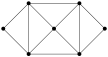
\includegraphics[width=\linewidth]{./img/image-107.svg}
\end{sbspanel}%
\end{sidebyside}%
\par
%
\begin{enumerate}
\item{}Find a subgraph with the smallest number of edges that is still connected and contains all the vertices.%
\item{}Find a subgraph with the largest number of edges that doesn't contain any cycles.%
\item{}What do you notice about the number of edges in your examples above?  Is this a coincidence?%
\end{enumerate}
%
\end{investigation}%
\begin{assemblage}{Definition of a Tree.}{p:assemblage:kYk}%
A \terminology{tree} is a connected graph containing no cycles.\footnotemark{}%
\par
A \terminology{forest} is a graph containing no cycles.   Note that this means that a connected forest is a tree.%
\end{assemblage}
\footnotetext[1]{Sometimes this is stated as ``a tree is an acyclic connected graph;'' ``acyclic'' is just a fancy word for ``containing no cycles.''\label{g:fn:idm233526672960}}%
\begin{activity}{}{g:activity:idm233526670080}%
%
\begin{enumerate}
\item{}Draw all trees on five vertices.%
\item{}Draw a tree with exactly two leaves.%
\item{}Draw a tree with exactly three leaves.%
\item{}What must be true about the degree sequence of a tree?%
\end{enumerate}
\end{activity}%
We wish to really understand trees. This means we should discover properties of trees; what makes them special and what is special about them.%
\par
A tree is a connected graph with no cycles. Is there anything else we can say? It would be nice to have other equivalent conditions for a graph to be a tree. That is, we would like to know whether there are any graph theoretic properties that all trees have, and perhaps even that \emph{only} trees have.%
\par
To get a feel for the sorts of things we can say, we will consider three \emph{propositions} about trees.  These will also illustrate important proof techniques that apply to graphs in general, and happen to be a little easier for trees.%
\par
Our first proposition gives an alternate definition for a tree.  That is, it gives necessary and sufficient conditions for a graph to be a tree.%
\begin{proposition}{}{}{x:proposition:prop-unique-paths-trees}%
A graph \(T\) is a tree if and only if between every pair of distinct vertices of \(T\) there is a unique path.%
\end{proposition}
\begin{proof}{}{p:proof:zbP}
This is an ``if and only if'' statement, so we must prove two implications.  We start by proving that if \(T\) is a tree, then between every pair of distinct vertices there is a unique path.%
\par
Assume \(T\) is a tree, and let \(u\) and \(v\) be distinct vertices (if \(T\) only has one vertex, then the conclusion is satisfied automatically).  We must show two things to show that there is a unique path between \(u\) and \(v\): that there is a path, and that there is not more than one path.  The first of these is automatic, since \(T\) is a tree, it is connected, so there is a path between any pair of vertices.%
\par
To show the path is unique, we suppose there are two paths between \(u\) and \(v\), and get a contradiction.  The two paths might start out the same, but since they are different, there is some first vertex \(u'\) after which the two paths diverge.  However, since the two paths both end and \(v\), there is some first vertex after \(u'\) that they have in common, call it \(v'\).  Now consider the two paths from \(u'\) to \(v'\).  Taken together, these form a cycle, which contradicts our assumption that \(T\) is a tree.%
\par
Now we consider the converse: if between every pair of distinct vertices of \(T\) there is a unique path, then \(T\) is a tree.  So assume the hypothesis: between every pair of distinct vertices of \(T\) there is a unique path.  To prove that \(T\) is a tree, we must show it is connected and contains no cycles.%
\par
The first half of this is easy: \(T\) is connected, because there is a path between every pair of vertices.  To show that \(T\) has no cycles, we assume it does, for the sake of contradiction.  Let \(u\) and \(v\) be two distinct vertices in a cycle of \(T\).  Since we can get from \(u\) to \(v\) by going clockwise or counterclockwise around the cycle, there are two paths from \(u\) and \(v\), contradicting our assumption.%
\par
We have established both directions so we have completed the proof.%
\end{proof}
\begin{corollary}{}{}{x:corollary:cor-unique-paths-forests}%
A graph \(F\) is a forest if and only if between any pair of vertices in \(F\) there is at most one path.%
\end{corollary}
\index{leaf} Our second proposition tells us that all trees have \terminology{leaves}: vertices of degree one.%
\begin{proposition}{}{}{x:proposition:prop-leaves-in-trees}%
Any tree with at least two vertices has at least two vertices of degree one.%
\end{proposition}
\begin{proof}{}{p:proof:fiY}
We give a proof by contradiction.  Let \(T\) be a tree with at least two vertices, and suppose, contrary to stipulation, that there are not two vertices of degree one.%
\par
Let \(P\) be a path in \(T\) of longest possible length.  Let \(u\) and \(v\) be the endpoints of the path.  Since \(T\) does not have two vertices of degree one, at least one of these must have degree two or higher.  Say that it is \(u\).  We know that \(u\) is adjacent to a vertex in the path \(P\), but now it must also be adjacent to another vertex, call it \(u'\).%
\par
Where is \(u'\)?  It cannot be a vertex of \(P\), because if it was, there would be two distinct paths from \(u\) to \(u'\): the edge between them, and the first part of \(P\) (up to \(u'\)).  But \(u'\) also cannot be outside of \(P\), for if it was, there would be a path from \(u'\) to \(v\) that was longer than \(P\), which has longest possible length.%
\par
This contradiction proves that there must be at least two vertices of degree one.  In fact, we can say a little more: \(u\) and \(v\) must \emph{both} have degree one.%
\end{proof}
The proposition is quite useful when proving statements about trees, because we often prove statements about trees by \emph{induction}.  To do so, we need to reduce a given tree to a smaller tree (so we can apply the inductive hypothesis).  Getting rid of a vertex of degree one is an obvious choice, and now we know there is always one to get rid of.%
\par
To illustrate how induction is used on trees, we will consider the relationship between the number of vertices and number of edges in trees.  Is there a tree with exactly 7 vertices and 7 edges?  Try to draw one.  Could a tree with 7 vertices have only 5 edges?  There is a good reason that these seem impossible to draw.%
\begin{proposition}{}{}{x:proposition:prop-tree-edge-vertex}%
\index{tree!number of edges and vertices}%
Let \(T\) be a tree with \(v\) vertices and \(e\) edges.  Then \(e = v-1\).%
\end{proposition}
\begin{proof}{}{p:proof:Lqh}
We will give a proof by induction on the number of vertices in the tree.  That is, we will prove that every tree with \(v\) vertices has exactly \(v-1\) edges, and then use induction to show this is true for all \(v \ge 1\).%
\par
For the base case, consider all trees with \(v = 1\) vertices.  There is only one such tree: the graph with a single isolated vertex.  This graph has \(e = 0\) edges, so we see that \(e = v-1\) as needed.%
\par
Now for the inductive case, fix \(k \ge 1\) and assume that all trees with \(v=k\) vertices have exactly \(e=k-1\) edges.  Now consider an arbitrary tree \(T\) with \(v = k+1\) vertices.  By \hyperref[x:proposition:prop-leaves-in-trees]{Proposition~{\xreffont\ref{x:proposition:prop-leaves-in-trees}}}, \(T\) has a vertex \(v_0\) of degree one.  Let \(T'\) be the tree resulting from removing \(v_0\) from \(T\) (together with its incident edge).  Since we removed a leaf, \(T'\) is still a tree (the unique paths between pairs of vertices in \(T'\) are the same as the unique paths between them in \(T\)).%
\par
Now \(T'\) has \(k\) vertices, so by the inductive hypothesis, has \(k-1\) edges.  What can we say about \(T\)?  Well, it has one more edge than \(T'\), so it has \(k\) edges.  But this is exactly what we wanted: \(v=k+1\), \(e=k\) so indeed \(e = v-1\).  This completes the inductive case, and the proof.%
\end{proof}
In fact, more is true.%
\begin{proposition}{}{}{g:proposition:idm233527745840}%
If a connected graph \(G\) has \(v\) vertices and \(v-1\) edges, then \(G\) is a tree.%
\end{proposition}
\begin{proof}{}{g:proof:idm233527743728}
Suppose \(G\) is connected, has \(v\) vertices, and \(v-1\) edges. If \(G\) is not a tree, then it must have at least one cycle (since it's connected). If we remove one edge \(e_1\) from its cycle, then \(G_1 = G\setminus e_1\) is still connected. If \(G_1\) has a cycle, then remove \(e_2\) from the cycle to obtain \(G_2\), which must still be connected. Continue in this way to obtain a connected graph \(G_k\) with no cycles, which must be a tree. Additionally, \(G_k\) is \(G\) with \(k\) edges removed, so it has \(v-1-k\) edges. However, since \(G_k\) has \(v\) vertices and is a tree, \hyperref[x:proposition:prop-tree-edge-vertex]{Proposition~{\xreffont\ref{x:proposition:prop-tree-edge-vertex}}}  must have \(v-1\) edges, which is a contradiction unless \(k=0\), in which case \(G\) had no cycles to begin with. Thus, \(G\) is a tree.%
\end{proof}
\end{subsubsectionptx}
\end{subsectionptx}
%
%
\typeout{************************************************}
\typeout{Subsection 13.2.2 Today's Screencast}
\typeout{************************************************}
%
\begin{subsectionptx}{Today's Screencast}{}{Today's Screencast}{}{}{g:subsection:idm233527743472}
\begin{insight}{}{g:insight:idm233527743008}%
\end{insight}
\end{subsectionptx}
%
%
\typeout{************************************************}
\typeout{Subsection 13.2.3 If you missed class today}
\typeout{************************************************}
%
\begin{subsectionptx}{If you missed class today}{}{If you missed class today}{}{}{g:subsection:idm233527733328}
%
\begin{enumerate}
\item{}Work through today's outline and read the marked pages in the book.%
\item{}Watch the screencast above.%
\item{}Submit any homework\slash{}assignments due today (check our \href{https://dordt.instructure.com/courses/3110050}{Canvas course} or the \href{https://prof.mkjanssen.org/ds/index.html\#schedule}{syllabus schedule} to see what's due).%
\item{}\href{mailto:mike.janssen@dordt.edu}{Send Dr. Janssen an email} or \href{https://calendly.com/mkjanssen/student-hours}{set up a student hours appointment} if you have any questions!%
\end{enumerate}
\end{subsectionptx}
\end{sectionptx}
\end{chapterptx}
%
%
\typeout{************************************************}
\typeout{Chapter 14 Week 14: Apr. 12-Apr. 16}
\typeout{************************************************}
%
\begin{chapterptx}{Week 14: Apr. 12-Apr. 16}{}{Week 14: Apr. 12-Apr. 16}{}{}{x:chapter:Week-14}
%
%
\typeout{************************************************}
\typeout{Section 14.1 Apr. 12: Trees II}
\typeout{************************************************}
%
\begin{sectionptx}{Apr. 12: Trees II}{}{Apr. 12: Trees II}{}{}{x:section:Apr-12}
\begin{introduction}{}%
\begin{assemblage}{Motivating Questions.}{g:assemblage:idm233527727280}%
Here are some questions we'll consider. %
\begin{enumerate}
\item{}\#%
\item{}%
\item{}%
\end{enumerate}
%
\end{assemblage}
\end{introduction}%
%
%
\typeout{************************************************}
\typeout{Subsection 14.1.1 Outline}
\typeout{************************************************}
%
\begin{subsectionptx}{Outline}{}{Outline}{}{}{g:subsection:idm233527726256}
Today's material comes from \href{http://discrete.openmathbooks.org/dmoi3/sec_trees.html}{Section 4.2} of the book. You're encouraged to read it before coming to class.%
%
%
\typeout{************************************************}
\typeout{Subsubsection 14.1.1.1 Rooted Trees}
\typeout{************************************************}
%
\begin{subsubsectionptx}{Rooted Trees}{}{Rooted Trees}{}{}{g:subsubsection:idm233527724016}
\index{rooted tree}%
\index{tree!rooted}%
So far, we have thought of trees only as a particular kind of graph. However, it is often useful to add additional structure to trees to help solve problems. Data is often structured like a tree. This book, for example, has a tree structure: draw a vertex for the book itself. Then draw vertices for each chapter, connected to the book vertex. Under each chapter, draw a vertex for each section, connecting it to the chapter it belongs to. The graph will not have any cycles; it will be a tree. But a tree with clear hierarchy which is not present if we don't identify the book vertex as the ``top''.%
\par
\index{root (in a tree)} As soon as one vertex of a tree is designated as the \terminology{root}, then every other vertex on the tree can be characterized by its position relative to the root.  This works because there is a unique path between any two vertices in a tree.  So from any vertex, we can travel back to the root in exactly one way.  This also allows us to describe how distinct vertices in a rooted tree are related.%
\par
\index{parent (in a rooted tree)}\index{child (in a rooted tree)} If two vertices are adjacent, then we say one of them is the \terminology{parent} of the other, which is called the \terminology{child} of the parent.  Of the two, the parent is the vertex that is closer to the root.  Thus the root of a tree is a parent, but is not the child of any vertex (and is unique in this respect: all non-root vertices have \emph{exactly one} parent).%
\par
\index{descendant (in a rooted tree)}\index{ancestor (in a rooted tree)} Not surprisingly, the child of a child of a vertex is called the \terminology{grandchild} of the vertex (and it is the \terminology{grandparent}).  More in general, we say that a vertex \(v\) is a \terminology{descendent} of a vertex \(u\) provided \(u\) is a vertex on the path from \(v\) to the root.  Then we would call \(u\) an \terminology{ancestor} of \(v\).%
\par
\index{sibling (in a rooted tree)} For most trees (in fact, all except paths with one end the root), there will be pairs of vertices neither of which is a descendant of the other.  We might call these cousins or siblings.  In fact, vertices \(u\) and \(v\) are called \terminology{siblings} provided they have the same parent.  Note that siblings are never adjacent (do you see why?).%
\begin{example}{}{p:example:pId}%
Consider the tree below.%
\begin{sidebyside}{1}{0.325}{0.325}{0}%
\begin{sbspanel}{0.35}%
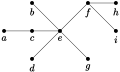
\includegraphics[width=\linewidth]{./img/img-labeled-tree.svg}
\end{sbspanel}%
\end{sidebyside}%
\par
If we designate vertex \(f\) as the root, then \(e\), \(h\), and \(i\) are the children of \(f\), and are siblings of each other.  Among the other things we cay say are that \(a\) is a child of \(c\), and a descendant of \(f\).  The vertex \(g\) is a descendant of \(f\), in fact, is a grandchild of \(f\).  Vertices \(g\) and \(d\) are siblings, since they have the common parent \(e\).%
\par
Notice how this changes if we pick a different vertex for the root.  If \(a\) is the root, then its lone child is \(c\), which also has only one child, namely \(e\).  We would then have \(f\) the child of \(e\) (instead of the other way around), and \(f\) is the descendant of \(a\), instead of the ancestor.  \(f\) and \(g\) are now siblings.%
\end{example}
\begin{example}{}{p:example:VPm}%
Explain why every tree is a bipartite graph.%
\par\smallskip%
\noindent\textbf{\blocktitlefont Solution}.\hypertarget{p:solution:rxq}{}\quad{}To show that a graph is bipartite, we must divide the vertices into two sets \(A\) and \(B\) so that no two vertices in the same set are adjacent.  Here is an algorithm that does just this.%
\par
Designate any vertex as the root.  Put this vertex in set \(A\).  Now put all of the children of the root in set \(B\).  None of these children are adjacent (they are siblings), so we are good so far.  Now put into \(A\) every child of every vertex in \(B\) (i.e., every grandchild of the root).  Keep going until all vertices have been assigned one of the sets, alternating between \(A\) and \(B\) every ``generation.''  That is, a vertex is in set \(B\) if and only if it is the child of a vertex in set \(A\).%
\end{example}
\index{breadth first search}\index{search!breadth first} The key to how we partitioned the tree in the example was to know which vertex to assign to a set next.  We chose to visit all vertices in the same generation before any vertices of the next generation.  This is usually called a \terminology{breadth first search} (we say ``search'' because you often traverse a tree looking for vertices with certain properties).%
\par
\index{depth first search}\index{search!depth first} In contrast, we could also have partitioned the tree in a different order.  Start with the root, put it in \(A\).  Then look for one child of the root to put in \(B\).  Then find a child of that vertex, into \(A\), and then find its child, into \(B\), and so on.  When you get to a vertex with no children, retreat to its parent and see if the parent has any other children.  So we travel as far from the root as fast as possible, then backtrack until we can move forward again.  This is called \terminology{depth first search}.%
\begin{theorem}{}{}{g:theorem:idm233527682400}%
Give a careful proof by induction on the number of vertices, that every tree is bipartite.%
\par\smallskip%
\noindentYou will need to remove a vertex of degree one, apply the inductive hypothesis to the result, and then say which set the degree one vertex to.%
\end{theorem}
\begin{proof}{}{g:proof:idm233527676160}
\end{proof}
\end{subsubsectionptx}
%
%
\typeout{************************************************}
\typeout{Subsubsection 14.1.1.2 Spanning Trees}
\typeout{************************************************}
%
\begin{subsubsectionptx}{Spanning Trees}{}{Spanning Trees}{}{}{g:subsubsection:idm233527723888}
\begin{assemblage}{Spanning tree.}{x:assemblage:assemblage-spanningtree}%
Given a connected graph \(G\), a \terminology{spanning tree} of \(G\) is a subgraph of \(G\) which is a tree and includes all the vertices of \(G\).%
\end{assemblage}
\begin{proposition}{}{}{g:proposition:idm233527672816}%
Every connected graph has a spanning tree.%
\end{proposition}
\begin{proof}{}{g:proof:idm233527669552}
How do we know?  We can give an algorithm for \emph{finding} a spanning tree!  Start with a connected graph \(G\).  If there is no cycle, then \(G\) is already a tree and we are done.  If there is a cycle, let \(e\) be any edge in that cycle and consider the new graph \(G_1 = G - e\) (i.e., the graph you get by deleting \(e\)).  This tree is still connected since \(e\) belonged to a cycle, there were at least two paths between its incident vertices.  Now repeat: if \(G_1\) has no cycles, we are done, otherwise define \(G_2\) to be \(G_1 - e_1\), where \(e_1\) is an edge in a cycle in \(G_1\).  Keep going.  This process must eventually stop, since there are only a finite number of edges to remove.  The result will be a tree, and since we never removed any vertex, a \emph{spanning} tree.%
\end{proof}
\begin{exploration}{}{g:exploration:idm233527669200}%
Find all spanning trees of the graph below. How many different spanning trees are there? How many different spanning trees are there \emph{up to isomorphism} (that is, if you grouped all the spanning trees by which are isomorphic, how many groups would you have)?%
\begin{image}{0.3}{0.4}{0.3}%
\includegraphics[width=\linewidth]{./img/img-114.svg}
\end{image}%
\end{exploration}%
\end{subsubsectionptx}
\end{subsectionptx}
%
%
\typeout{************************************************}
\typeout{Subsection 14.1.2 Today's Screencast}
\typeout{************************************************}
%
\begin{subsectionptx}{Today's Screencast}{}{Today's Screencast}{}{}{g:subsection:idm233527660752}
\begin{insight}{}{g:insight:idm233527660272}%
\end{insight}
\end{subsectionptx}
%
%
\typeout{************************************************}
\typeout{Subsection 14.1.3 If you missed class today}
\typeout{************************************************}
%
\begin{subsectionptx}{If you missed class today}{}{If you missed class today}{}{}{g:subsection:idm233527660144}
%
\begin{enumerate}
\item{}Work through today's outline and read the marked pages in the book.%
\item{}Watch the screencast above.%
\item{}Submit any homework\slash{}assignments due today (check our \href{https://dordt.instructure.com/courses/3110050}{Canvas course} or the \href{https://prof.mkjanssen.org/ds/index.html\#schedule}{syllabus schedule} to see what's due).%
\item{}\href{mailto:mike.janssen@dordt.edu}{Send Dr. Janssen an email} or \href{https://calendly.com/mkjanssen/student-hours}{set up a student hours appointment} if you have any questions!%
\end{enumerate}
\end{subsectionptx}
\end{sectionptx}
%
%
\typeout{************************************************}
\typeout{Section 14.2 Apr. 14: Planarity}
\typeout{************************************************}
%
\begin{sectionptx}{Apr. 14: Planarity}{}{Apr. 14: Planarity}{}{}{x:section:Apr-14}
\begin{introduction}{}%
\begin{assemblage}{Motivating Questions.}{g:assemblage:idm233527655056}%
Here are some questions we'll consider. %
\begin{enumerate}
\item{}What is a planar graph?%
\item{}What types of graphs are not planar?%
\end{enumerate}
%
\end{assemblage}
\end{introduction}%
%
%
\typeout{************************************************}
\typeout{Subsection 14.2.1 Outline}
\typeout{************************************************}
%
\begin{subsectionptx}{Outline}{}{Outline}{}{}{g:subsection:idm233527652896}
Today's material comes from \href{http://discrete.openmathbooks.org/dmoi3/sec_planar.html}{Section 4.3} of the book. You're encouraged to read it before coming to class.%
%
%
\typeout{************************************************}
\typeout{Subsubsection 14.2.1.1 Planar Graphs}
\typeout{************************************************}
%
\begin{subsubsectionptx}{Planar Graphs}{}{Planar Graphs}{}{}{g:subsubsection:idm233527651776}
\begin{investigation}{}{p:investigation:Mhf}%
\index{planar graph}%
\index{face (planar graph)}%
\index{planar graph}%
\index{face (planar graph)}%
When a connected graph can be drawn without any edges crossing, it is called \terminology{planar}. When a planar graph is drawn in this way, it divides the plane into regions called \terminology{faces}.%
\begin{enumerate}
\item{}Draw, if possible, two different planar graphs with the same number of vertices, edges, and faces.%
\item{}Draw, if possible, two different planar graphs with the same number of vertices and edges, but a different number of faces.%
\end{enumerate}
%
\end{investigation}%
\index{planar graph} When is it possible to draw a graph so that none of the edges cross? If this \emph{is} possible, we say the graph is \terminology{planar} (since you can draw it on the \emph{plane}).%
\par
\index{face (planar graph)}\index{planar region|see{face (planar graph)}}\index{region (graph)|see{face (planar graph)}} When a planar graph is drawn without edges crossing, the edges and vertices of the graph divide the plane into regions. We will call each region a \terminology{face}. The graph above has 3 faces (yes, we \emph{do} include the ``outside'' region as a face). The number of faces does not change no matter how you draw the graph (as long as you do so without the edges crossing), so it makes sense to ascribe the number of faces as a property of the planar graph.%
\par
WARNING: you can only count faces when the graph is drawn in a planar way.%
\par
There is a connection between the number of vertices (\(v\)), the number of edges (\(e\)) and the number of faces (\(f\)) in any connected planar graph. This relationship is called Euler's formula.%
\begin{theorem}{Euler's Formula for Planar Graphs.}{}{p:theorem:lPi}%
\index{Euler's formula for planar graphs}%
For any connected planar graph with \(v\) vertices, \(e\) edges and \(f\) faces, we have%
\begin{equation*}
v-e + f = 2\text{.}
\end{equation*}
%
\end{theorem}
\begin{proof}{}{g:proof:idm233527632144}
Begin with our graph \(G\) and identify a spanning tree \(T\) of \(G\). Let \(v_T, e_T,  f_T\) denote the corresponding number of each object of \(T\).%
\par
Observe that each time that we remove an edge of \(G\) not in \(T\), two faces merge. When we break all cycles of \(G\) (leaving us with a tree), we have a single face. Thus, we remove \(f-1\) edges from \(G\) to achieve \(T\), i.e.,%
\begin{equation*}
e - (f-1) = e_T\text{.}
\end{equation*}
Since \(T\) is a tree, we know that \(e_T = v_T - 1\), so \(v_T - e_T = 1\). The spanning tree has exactly one face, so \(f_T = 1\), and adding these two together give us \(v_T - e_T + f_T = 2\). Moreover, since \(T\) is a spanning tree, \(v_T = v\). Substituting this and \hyperref[x:me:eq-euler-formula-proof1]{Equation~} into \(v_T - e_T + f_T = 2\) we have \(v - (e-(f-1))+f_T = 2\), which simplifies to our desired result as \(f_T = 1\).%
\end{proof}
\end{subsubsectionptx}
%
%
\typeout{************************************************}
\typeout{Subsubsection 14.2.1.2 Non-planar graphs}
\typeout{************************************************}
%
\begin{subsubsectionptx}{Non-planar graphs}{}{Non-planar graphs}{}{}{g:subsubsection:idm233527629344}
\index{non-planar graph}%
\index{planar graph!non-planar graph}%
\begin{investigation}{}{p:investigation:qzb}%
For the complete graphs \(K_n\), we would like to be able to say something about the number of vertices, edges, and (if the graph is planar) faces. Let's first consider \(K_3\):%
\begin{enumerate}
\item{}How many vertices does \(K_3\) have? How many edges?%
\item{}If \(K_3\) is planar, how many faces should it have?%
\end{enumerate}
%
\par
Repeat parts (1) and (2) for \(K_4\), \(K_5\), and \(K_{23}\).%
\par
What about complete bipartite graphs? How many vertices, edges, and faces (if it were planar) does \(K_{7,4}\) have? For which values of \(m\) and \(n\) are \(K_n\) and \(K_{m,n}\) planar?%
\end{investigation}%
\begin{theorem}{}{}{p:theorem:RWr}%
\index{non-planar graph!k5@\(K_5\)}%
\index{planar graph!non-planar graph!k5@\(K_5\)}%
\(K_5\) is not planar.%
\end{theorem}
\begin{proof}{}{p:proof:Yvx}
The proof is by contradiction. So assume that \(K_5\) is planar. Then the graph must satisfy Euler's formula for planar graphs. \(K_5\) has 5 vertices and 10 edges, so we get%
\begin{equation*}
5 - 10 + f = 2\text{,}
\end{equation*}
which says that if the graph is drawn without any edges crossing, there would be \(f = 7\) faces.%
\par
Now consider how many edges surround each face. Each face must be surrounded by at least 3 edges. Let \(B\) be the total number of \emph{boundaries} around all the faces in the graph. Thus we have that \(3f \le B\). But also \(B = 2e\), since each edge is used as a boundary exactly twice. Putting this together we get%
\begin{equation*}
3f \le 2e\text{.}
\end{equation*}
%
\par
But this is impossible, since we have already determined that \(f = 7\) and \(e = 10\), and \(21 \not\le 20\). This is a contradiction so in fact \(K_5\) is not planar.%
\end{proof}
The other simplest graph which is not planar is \(K_{3,3}\)%
\begin{sidebyside}{1}{0.4}{0.4}{0}%
\begin{sbspanel}{0.2}%
\resizebox{\linewidth}{!}{%
\begin{tikzpicture}[yscale=1.2]
          \draw (-1,1) \v -- (-1,0)\v  -- (0,1) \v -- (0,0) \v -- (1,1) \v -- (1,0) \v -- (0,1) -- (-1,0) -- (1,1) (1,0) -- (-1,1) -- (0,0);
        \end{tikzpicture}
}%
\end{sbspanel}%
\end{sidebyside}%
\par
Proving that \(K_{3,3}\) is not planar answers the houses and utilities puzzle: it is not possible to connect each of three houses to each of three utilities without the lines crossing.%
\begin{theorem}{}{}{p:theorem:ydA}%
\index{non-planar graph!k33@\(K_{3,3}\)}%
\index{planar graph!non-planar graph!k33@\(K_{3,3}\)}%
\(K_{3,3}\) is not planar.%
\end{theorem}
\begin{proof}{}{p:proof:ECG}
Again, we proceed by contradiction. Suppose \(K_{3,3}\) were planar. Then by Euler's formula there will be 5 faces, since \(v = 6\), \(e = 9\), and \(6 - 9 + f = 2\).%
\par
How many boundaries surround these 5 faces? Let \(B\) be this number. Since each edge is used as a boundary twice, we have \(B = 2e\). Also, \(B \ge 4f\) since each face is surrounded by 4 or more boundaries. We know this is true because \(K_{3,3}\) is bipartite, so does not contain any 3-edge cycles. Thus%
\begin{equation*}
4f \le 2e\text{.}
\end{equation*}
%
\par
But this would say that \(20 \le 18\), which is clearly false. Thus \(K_{3,3}\) is not planar.%
\end{proof}
\begin{theorem}{}{Kuratowski (1930)}{g:theorem:idm233527580592}%
A finite graph is planar if and only if it does not contain a subgraph that is a subdivision\begin{aside}{}{g:aside:idm233527579616}%
\end{aside}
 of \(K_5\) or \(K_{3,3}\).%
\end{theorem}
\end{subsubsectionptx}
\end{subsectionptx}
%
%
\typeout{************************************************}
\typeout{Subsection 14.2.2 Today's Screencast}
\typeout{************************************************}
%
\begin{subsectionptx}{Today's Screencast}{}{Today's Screencast}{}{}{g:subsection:idm233527576496}
\begin{insight}{}{g:insight:idm233527576112}%
\end{insight}
\end{subsectionptx}
%
%
\typeout{************************************************}
\typeout{Subsection 14.2.3 If you missed class today}
\typeout{************************************************}
%
\begin{subsectionptx}{If you missed class today}{}{If you missed class today}{}{}{g:subsection:idm233527575984}
%
\begin{enumerate}
\item{}Work through today's outline and read the marked pages in the book.%
\item{}Watch the screencast above.%
\item{}Submit any homework\slash{}assignments due today (check our \href{https://dordt.instructure.com/courses/3110050}{Canvas course} or the \href{https://prof.mkjanssen.org/ds/index.html\#schedule}{syllabus schedule} to see what's due).%
\item{}\href{mailto:mike.janssen@dordt.edu}{Send Dr. Janssen an email} or \href{https://calendly.com/mkjanssen/student-hours}{set up a student hours appointment} if you have any questions!%
\end{enumerate}
\end{subsectionptx}
\end{sectionptx}
%
%
\typeout{************************************************}
\typeout{Section 14.3 Apr. 16}
\typeout{************************************************}
%
\begin{sectionptx}{Apr. 16}{}{Apr. 16}{}{}{x:section:Apr-16}
\end{sectionptx}
\end{chapterptx}
%
%
\typeout{************************************************}
\typeout{Chapter 15 Week 15: Apr. 19-Apr. 23}
\typeout{************************************************}
%
\begin{chapterptx}{Week 15: Apr. 19-Apr. 23}{}{Week 15: Apr. 19-Apr. 23}{}{}{x:chapter:Week-15}
%
%
\typeout{************************************************}
\typeout{Section 15.1 Apr. 19}
\typeout{************************************************}
%
\begin{sectionptx}{Apr. 19}{}{Apr. 19}{}{}{x:section:Apr-19}
\end{sectionptx}
%
%
\typeout{************************************************}
\typeout{Section 15.2 Apr. 21}
\typeout{************************************************}
%
\begin{sectionptx}{Apr. 21}{}{Apr. 21}{}{}{x:section:Apr-21}
\end{sectionptx}
%
%
\typeout{************************************************}
\typeout{Section 15.3 Apr. 23}
\typeout{************************************************}
%
\begin{sectionptx}{Apr. 23}{}{Apr. 23}{}{}{x:section:Apr-23}
\end{sectionptx}
\end{chapterptx}
%
%
\typeout{************************************************}
\typeout{Chapter 16 Week 16: Apr. 26-Apr. 30}
\typeout{************************************************}
%
\begin{chapterptx}{Week 16: Apr. 26-Apr. 30}{}{Week 16: Apr. 26-Apr. 30}{}{}{x:chapter:Week-16}
%
%
\typeout{************************************************}
\typeout{Section 16.1 Apr. 26}
\typeout{************************************************}
%
\begin{sectionptx}{Apr. 26}{}{Apr. 26}{}{}{x:section:Apr-26}
\end{sectionptx}
%
%
\typeout{************************************************}
\typeout{Section 16.2 Apr. 28}
\typeout{************************************************}
%
\begin{sectionptx}{Apr. 28}{}{Apr. 28}{}{}{x:section:Apr-28}
\end{sectionptx}
%
%
\typeout{************************************************}
\typeout{Section 16.3 Apr. 30}
\typeout{************************************************}
%
\begin{sectionptx}{Apr. 30}{}{Apr. 30}{}{}{x:section:Apr-30}
\end{sectionptx}
\end{chapterptx}
%
%% A lineskip in table of contents as transition to appendices, backmatter
\addtocontents{toc}{\vspace{\normalbaselineskip}}
%
%
%% The index is here, setup is all in preamble
%% Index locators are cross-references, so same font here
{\xreffont\printindex}
%
%
%
\typeout{************************************************}
\typeout{Appendix A Counting Techniques}
\typeout{************************************************}
%
%
\appendix
%
\begin{appendixptx}{Counting Techniques}{}{Counting Techniques}{}{}{x:appendix:appendix-counting}
Throughout the course, we'll collect lots of ways to count things. However, they often seem really similar to one another, so in this appendix I will try to collect various archetypal problems and methodologies. This will be a work in progress.%
%
%
\typeout{************************************************}
\typeout{Section A.1 Additive and Multiplicative Principles}
\typeout{************************************************}
%
\begin{sectionptx}{Additive and Multiplicative Principles}{}{Additive and Multiplicative Principles}{}{}{g:section:idm233527563440}
First, recall the statements of the \hyperref[x:assemblage:additive-principle]{Additive Principle} and \hyperref[x:assemblage:multiplicative-principle]{Multiplicative Principle}.%
\par
Both involve independent events; the difference between the two is therefore the difference between ``or'' and ``and''.%
\begin{question}{The Additive Principle Question.}{g:question:idm233527558640}%
If event \(A\) can occur in \(m\) ways and event \(B\) occurs independently of \(A\) in \(n\) ways, how many ways can \(A\) or \(B\) occur?%
\end{question}
\begin{example}{}{g:example:idm233527558000}%
Lila's Sweet Shop sells \(m\) types of ice cream and \(n\) types of frozen yogurt. There are then \(m+n\) ways to get a single scoop of frozen yogurt \emph{or} ice cream (additive principle) and \(m\cdot n\) ways to get one scoop of frozen yogurt \emph{and} one scoop of ice cream (multiplicative principle).%
\end{example}
\end{sectionptx}
%
%
\typeout{************************************************}
\typeout{Section A.2 PIE}
\typeout{************************************************}
%
\begin{sectionptx}{PIE}{}{PIE}{}{}{g:section:idm233527554384}
\end{sectionptx}
%
%
\typeout{************************************************}
\typeout{Section A.3 Binomial Coefficients}
\typeout{************************************************}
%
\begin{sectionptx}{Binomial Coefficients}{}{Binomial Coefficients}{}{}{g:section:idm233527551008}
\begin{question}{The Binomial Coefficient Question, version 1.}{g:question:idm233527550624}%
How many ways are there to choose \(k\) objects from \(n\) objects? (Assuming \(k \lt n\), of course.)%
\end{question}
\begin{question}{The Binomial Coefficient Question, version 2 (DMWD).}{g:question:idm233527548352}%
How many ways are there to place \(k\) identical (unlabeled) balls, at most one per box, into \(n\) labeled boxes? (Assuming \(k \lt n\), of course.)%
\end{question}
\begin{question}{}{g:question:idm233527546112}%
Why are the previous two questions equivalent?%
\end{question}
\end{sectionptx}
%
%
\typeout{************************************************}
\typeout{Section A.4 Permutations}
\typeout{************************************************}
%
\begin{sectionptx}{Permutations}{}{Permutations}{}{}{g:section:idm233527545600}
This is a question answered by counting \emph{permutations}. Recall \hyperref[x:assemblage:formula-permutations]{the formula}.%
\end{sectionptx}
%
%
\typeout{************************************************}
\typeout{Section A.5 Stars and Bars}
\typeout{************************************************}
%
\begin{sectionptx}{Stars and Bars}{}{Stars and Bars}{}{}{g:section:idm233527543664}
\end{sectionptx}
%
%
\typeout{************************************************}
\typeout{Section A.6 Anagrams}
\typeout{************************************************}
%
\begin{sectionptx}{Anagrams}{}{Anagrams}{}{}{g:section:idm233527543280}
\end{sectionptx}
\end{appendixptx}
%
\backmatter
%
\end{document}